\chapter{Sparse Representation of Multivariate Extremes}
\label{jmva}

%XXX TODO: detailed remark on classification in extreme regions (add classif in background?)

\begin{chapabstract}
This chapter presents the details relative to the introducing Section~\ref{resume:sec:JMVA}.

Capturing the dependence structure of multivariate extreme events is
a major concern in many fields involving the management of risks
stemming from multiple sources, \emph{e.g.}~portfolio monitoring, insurance, environmental risk management and anomaly detection.
One convenient (non-parametric) characterization of  extreme dependence in the
framework of multivariate Extreme Value Theory (EVT) is the \textit{angular
  measure}, which provides direct information about the probable
'directions' of extremes, that is, the relative contribution of each
feature/coordinate of the `largest' observations. Modeling the
angular measure in high dimensional problems is a major challenge for
the multivariate analysis of rare events.
The present chapter proposes a novel methodology aiming at 
exhibiting a sparsity pattern within the dependence structure of extremes. 
This is achieved by estimating the amount of mass spread by the angular measure on
representative sets of directions, corresponding to  specific sub-cones of $\mathbb{R}_+^d$.
This dimension reduction technique  paves the way towards scaling up existing multivariate EVT methods.
Beyond a non-asymptotic study providing a theoretical validity
framework for our method, we propose  as a direct application a --first--
Anomaly Detection algorithm based on \textit{multivariate} EVT.  This algorithm builds a sparse `normal profile' of extreme behaviors, to be confronted with new (possibly abnormal) extreme observations. Illustrative experimental results provide strong empirical evidence of the relevance of our approach.
\end{chapabstract}

Note: The material of this chapter is based on previous work under review available in \cite{ARXIV16}. Part of this work have been published in \cite{AISTAT15} and \cite{NIPSWORKSHOP15}.



\section{Introduction}
\label{jmva:sec:intro}
% An anomaly (or outlier) is `an observation which deviates so much from other observations as to arouse suspicions that it was generated by a different mechanism' (\cite{Hawkins1980}).
% According to a further definition from Barnett and Lewis \cite{Barnett94}, this is an observation (or subset of observations) `which appears to be inconsistent with the remainder of that set of data'.
% These definitions give a hunch of what an outlying observation is, and motivate many anomaly detection methods whose approach is statistical (\cite{Eskin2000}, \cite{Desforges1998}, \cite{Barnett94}, \cite{Hawkins1980}), distance based (\cite{Knorr98}, \cite{Knorr2000}, \cite{Eskin2002geometric}), local-density based (\cite{Breunig2000LOF}, \cite{Breunig99LOF}, \cite{Tang2002enhancing}, \cite{Papadimitriou2003loci} ), spectral based (\cite{Shyu2003}, \cite{Wang2006}, \cite{Lee2013}) and others (\cite{Aggarwal2001}, \cite{Kriegel2008}, \cite{Liu2008}). The approach discussed in this paper lies at the intersection of the non-parametric statistical and the spectral one.

\subsection{Context: multivariate extreme values in large dimension}

Extreme Value Theory (EVT in abbreviated form) provides a theoretical basis for
modeling the tails of probability  distributions. In many applied fields where 
rare events  may have a disastrous impact, such as 
finance, insurance, climate,  environmental risk management, network
monitoring (\cite{finkenstadt2003extreme,smith2003statistics}) or  
anomaly detection (\cite{Clifton2011,Lee2008}), the information carried by extremes is crucial. In a multivariate context, the dependence structure
of the joint tail is of particular interest, as it gives access
\emph{e.g.} to probabilities of a joint excess above high thresholds or
to multivariate quantile regions. Also, the distributional structure of
extremes indicates which components of a multivariate quantity may be
simultaneously large while the others stay small, which is a valuable
piece of information for multi-factor risk assessment or
detection of anomalies among other --not abnormal--  extreme data. 



In a multivariate `Peak-Over-Threshold' setting, realizations of a $d$ -dimensional random vector $\mb Y = (Y_1 ,..., Y_d)$ are observed and the goal pursued is to learn the conditional distribution of excesses, $\left[~ \mb Y ~|~ \|\mb Y\| \ge  r ~ \right]$, above some large threshold $ r>0$.
The dependence structure of such excesses is described via the
distribution of the ‘directions’ formed by the most extreme
observations, the  so-called \emph{angular measure}, hereafter denoted by $\Phi$.  The latter
is defined on the positive orthant of the $d-1$ dimensional
hyper-sphere. To wit, for any region $A$  on the unit sphere (a set
of `directions'), after suitable standardization of the data (see
 Section~\ref{jmva:sec:framework}), 
$C \Phi(A) \simeq \PP(\|\mb Y\|^{-1} \mb Y \in A ~|~ \|\mb Y\| >r)$, where $C$ is a normalizing constant. 
Some probability mass may be spread on any sub-sphere of dimension $k
< d$, the $k$-faces of an hyper-cube if we use the infinity norm, which
complexifies inference when $d$ is large. To fix ideas, the presence of $\Phi$-mass on a
sub-sphere of the type $\{\max_{1\leq i\leq k} x_i = 1 ~;~   x_i >0 \;(i\le k) ~;~  x_{k+1} = \ldots = x_d = 0\}$ indicates that the components $Y_1,\ldots,Y_k$ may
simultaneously be large, while the others are small.
An extensive exposition of this multivariate extreme setting may be found \eg~in \cite{Resnick1987},~\cite{BGTS04}. 


%%%%%%%%%%%%%%%%%%%%%%%

Parametric or semi-parametric modeling and estimation of the structure of
multivariate extremes is relatively well documented in the statistical literature, see \emph{e.g.} \cite{coles1991modeling,fougeres2009models,cooley2010pairwise,sabourinNaveau2012} and the references therein. In a non-parametric setting, there is also an abundant literature concerning consistency and asymptotic normality of estimators of functionals characterizing the extreme dependence structure, \eg~extreme value copulas or the \emph{stable tail dependence function} (\stdf), see \cite{Segers12Bernoulli, Drees98, Embrechts2000, Einmahl2012, dHF06}.

In many applications, it is nevertheless more convenient to work with the angular measure itself, as the latter gives more direct information on the dependence structure and is able to reflect structural simplifying properties (\eg~sparsity as detailed below) which would not appear in copulas or in the \stdf.
However, non-parametric modeling of the angular measure faces major difficulties, stemming from the potentially complex structure of the latter, especially in a high dimensional setting.
Further, from a theoretical point of view, non-parametric estimation of the angular measure has only been studied in the two dimensional case, in \cite{Einmahl2001} and \cite{Einmahl2009}, in an asymptotic framework.

%%%%%%%%%%%%%%%%%%%%%%%
{Scaling up multivariate EVT} is a major challenge that one
faces when confronted to high-dimensional learning
tasks, since most multivariate extreme value models have been
designed to handle moderate dimensional problems (say, of dimensionality  $d\le 10$). % that one faces when it comes to applying it in a
% machine learning context.
% In addition, their practical use is
%  restricted to moderate dimensional problems (say, $d\le 10$), 
For larger dimensions, 
 simplifying modeling choices are needed,
 stipulating \emph{e.g} that only some pre-definite subgroups of components
 may be concomitantly extremes, or, on the contrary, that all of them
 must be (see  \emph{e.g.} 
 \cite{stephenson2009high} or \cite{sabourinNaveau2012}).
This curse of dimensionality can be explained, in the context of
extreme values analysis, by the relative  scarcity of extreme  data,
the  computational
complexity of the estimation procedure and, in the parametric case, by 
the fact that the dimension of the parameter space usually grows with
that of the sample space. This calls for dimensionality reduction devices
adapted to multivariate extreme values.

In a wide range of situations, one may expect the occurrence of two phenomena:

\noindent
\textbf{1-} Only a `small' number of groups of components may be concomitantly extreme, so that only a `small' number of hyper-cubes (those corresponding to these subsets of indexes precisely) have non zero mass (`small' is relative to the total number of groups $2^d$).

\noindent
\textbf{2-} Each of these groups contains a limited number of coordinates (compared to the original dimensionality), so that the corresponding hyper-cubes with non zero mass have small dimension compared to $d$.

\noindent
The main purpose of this chapter is to introduce a data-driven
methodology for identifying such faces, so as to reduce the
dimensionality of the problem and thus to learn a sparse 
representation  of extreme behaviors. 
In case hypothesis \textbf{2-} is not fulfilled, such a sparse  `profile' can still be learned, but looses the low dimensional property of its supporting hyper-cubes.

One major issue is that real data generally do not concentrate on sub-spaces of zero Lebesgue measure. This is circumvented by setting to zero any coordinate less than a threshold $\epsilon>0$, so that the corresponding `angle' is assigned to a lower-dimensional face. 






% restrictive structural assumptions have to be
%  made

% Several multivariate models have been proposed, in a parametric
% context or in a semi-parametric one. However in practice, the applicability of
% these models is restricted to moderate dimensional problems (say $d\le
% 10$), 
% From a theoretical point of view, non-parametric
% estimators of  the \emph{stable tail dependence function} (another summary functional of the extremal
% dependence structure) have been proved to be  asymptotically
% normal.


% consistency and asymptotic normality of non-parametric estimators of the so-called
% \emph{angular measure} (which rules the distribution of the
% `directions' of the most extreme observations and uniquely determines
% the dependence structure of extremes)  has been established for the
% bivariate case only.  In dimension greater than three, 

%  However, the latter does not give direct access to the angular
% measure, nor does it allow to exhibit sparsity  in the latter, 


The theoretical results stated in this chapter build on the work
of % are clearly stated in this
% work, in the continuity of
\cite{COLT15} exposed in Chapter~\ref{colt}, where non-asymptotic bounds related to the statistical performance of a non-parametric estimator of the \stdf, another functional measure of the dependence structure of extremes,  are established.  
However, even in the case of a sparse angular measure, the support of
the \stdf~would not be so, since the latter functional is  an
integrated version of the former (see~\eqref{jmva:eq:integratePhiLambda},
 Section~\ref{jmva:sec:framework}). Also, 
%tools from statistical learning theory,
in many applications, it is more convenient to work with % an alternative (distributional)
% representation,
 the {angular
  measure}. Indeed, it  provides
direct  information about the
probable `directions' of extremes, that is, the relative contribution
of each components of the `largest' observations  (where `large' may be 
understood \emph{e.g.} in the sense of the infinity norm on the input
space). We emphasize again that estimating these `probable relative contributions' is a major concern in many fields
involving  the management of risks from multiple sources.
To the best of our knowledge, non-parametric estimation of the angular
measure has only been treated in the two dimensional case, in
\cite{Einmahl2001} and \cite{Einmahl2009}, in an asymptotic
framework.

\noindent
\textbf{Main contributions.} The present contribution extends the non-asymptotic study derived in Chapter~\ref{colt} to the angular measure of extremes, restricted to a well-chosen representative class of sets, corresponding to lower-dimensional regions of the space. The objective is to learn a representation of the angular measure, rough enough to
control the variance in high dimension and accurate enough to gain information about the 'probable directions' of extremes. This yields a --first-- non-parametric estimate of the angular measure in any dimension, restricted to a
class of sub-cones, with a non asymptotic bound on the error. 
 The representation thus obtained is exploited to detect anomalies among extremes. 

The proposed algorithm  is based on \textit{dimensionality
  reduction}. %, and can also be used as a preprocessing step to reduce the number of r.v.'s under consideration at extreme levels. % , as multivariate EVT is often inapplicable in a large dimensional context. XXX.
We believe that our method can also be used as a preprocessing stage, for dimensionality reduction purpose, before proceeding with a parametric or semi-parametric estimation which could benefit from the structural information issued in the first step. Such applications are beyond the scope of this work and will be the subject of further research.

\subsection{Application to Anomaly Detection}
% Anomaly Detection (AD in short, and depending of the application domain, outlier detection, novelty detection, deviation detection, exception mining) generally consists in assuming that the dataset under study contains a \textit{small} number of anomalies, generated by distribution models that  \textit{differ} from that generating the vast majority of the data.
%  % anomalies are a \textit{small} number of observations generated by \textit{different} models from the one generating the rest of the data
% %\sout{ -- the only difference in novelty detection is that the novel patterns are incorporated into the normal model after being detected. }.
% This formulation motivates many statistical AD methods, based on the underlying assumption that anomalies occur in low probability regions of the data generating process. Here and hereafter, the term `normal data' does not refer to Gaussian distributed data, but  to  \emph{not abnormal} ones, \ie~data belonging to the above mentioned majority. 
% Classical parametric techniques, like those developed in \cite{Barnett94} or in \cite{Eskin2000}, assume that the normal data are generated by a distribution belonging to some  specific, known in advance parametric model.  
% The most popular non-parametric approaches include algorithms based on density (level set) estimation (see \textit{e.g.} \cite{Scholkopf2001},  \cite{Scott2006} or \cite{Breunig99LOF}), on dimensionality reduction (\textit{cf} \cite{Shyu2003}, \cite{Aggarwal2001}) or on decision trees (\cite{Liu2008}).
% % %approach is statistical, \
% % % {\red donner le theme de chaque papier cité}
% % \cite{Eskin2000},
% % \cite{Desforges1998}, \cite{Barnett94}, \cite{Hawkins1980}
% % , distance
% % based, \cite{Knorr98}, \cite{Knorr2000}, \cite{Eskin2002geometric},
% % local-density based \cite{Breunig2000LOF}, \cite{Breunig99LOF},
% % \cite{Tang2002enhancing}, \cite{Papadimitriou2003loci}, spectral based
% % \cite{Shyu2003}, \cite{Wang2006}, \cite{Lee2013} and others
% % \cite{Aggarwal2001}, \cite{Kriegel2008}, \cite{Liu2008}. 
% One may refer to \cite{Hodge2004survey}, \cite{Chandola2009survey}, \cite{Patcha2007survey} and \cite{Markou2003survey} for excellent overviews of current research on Anomaly Detection, ad-hoc techniques being far too numerous to be listed here in an exhaustive manner.
The framework we develop in this chapter is non-parametric and lies at
the intersection of support estimation, density estimation and
dimensionality reduction: it consists in learning from training data
the support of a distribution, that can be decomposed into sub-cones,
hopefully of low dimension each and to which some mass is assigned,
according to %defining 
empirical versions of probability measures on %of specific 
extreme regions. 
%In addition, each subcone is (potentially) of low-dimension.
%\cite{hodge2004survey}:
%Anomalies arise because of human error, instrument error, natural deviations in populations, fraudulent behaviour, changes in behaviour of systems or faults in systems

% \textbf{Anomaly Ranking}. Most usual AD algorithms actually
% provide more than a predicted label for any new observation, abnormal vs. normal. Instead,
% they return a real valued function,  termed a \textit{scoring function} sometimes, defining a preorder/ranking on the input space. Such a function permits to rank any observations according to their supposed `degree of abnormality' and thresholding it yields a decision rule that splits the input space into `normal' and `abnormal' regions.
% In various fields (\textit{e.g.} fleet management, monitoring of energy/transportation networks), when confronted with massive data, being able to rank observations according to their degree of abnormality may significantly improve operational processes and allow for a prioritization of actions to be taken, especially in situations where human expertise required to check each observation is time-consuming.

% From a machine learning perspective, 
% % AD can be considered as a specific
% % classification task, where the usual assumption in supervised learning stipulating that the dataset contains structural
% % information regarding all classes breaks down, see
% % \cite{Roberts99}. This typically happens in the case of two highly
% % unbalanced classes: the normal class is expected to regroup a large
% % majority of the dataset, so that the very small number of points
% % representing the abnormal class does not allow to learn information
% % about this class. In a clustering based approach, it can be
% % interpreted as the presence of a single cluster, corresponding to the
% % normal data. The abnormal ones are too limited to share a commun
% % structure, \ie~to form a second cluster. Their only characteristic is
% % precisely to lie outside the normal cluster, namely to lack any
% % structure.  Thus, common classification approaches may not be applied
% % as such, even in a supervised
% % context. % That is the reason why even in a supervised framework, common classification approaches cannot be applied.
% \textit{supervised} AD consists in training the algorithm on a
% labeled (normal/abnormal) dataset including both normal and abnormal
% observations. In the \textit{semi-supervised} context, only normal
% data are available for training. This is the case in applications where
% normal operations are known but intrusion/attacks/viruses are unknown
% and should be detected. In the \textit{unsupervised} setup, no
% assumption is made on the data which consist in unlabeled normal and
% abnormal instances. \sout{Sometimes, no training is performed.} In general, 
%  a method from the semi-supervised framework may apply to the
% unsupervised one, as soon as the number of anomalies is sufficiently
% weak to prevent the algorithm from fitting them when learning the normal
% behavior. Such a method should be robust to outlying
% observations.

% \textbf{Connection to Extreme Value Theory} (EVT), which \textit{forms representations for the tails of distributions}, can be seen in the following sense. 
% In the unsupervised framework % (where the data set consists of a large number of normal data with a smaller unknown number of anomalies)

% As a matter of fact, `extreme' observations are often more susceptible to be anomalies than the others.
% % In the supervised or semi-supervised framework (that is, when the
% % algorithm is trained on normal data),  %considering only normal observations% where a dataset of only normal observations is available
% These extremal points represent the outlying regions of the normal instances. % we want to separate from the abnormal ones.
% In other words, extremal observations are often at the \textit{border} between normal and abnormal regions and play a very special role in this context.
% %
% As extreme observations constitute few percents of the data, a classical AD algorithm would tend to classify them as abnormal: it is not
% worth the risk (in terms of ROC or precision-recall curve for instance) trying to be more accurate in such low probability regions, without adapted tools. New
% observations outside the `observed support' are then most often predicted as abnormal.  However, false positives (\ie~false alarms) are very expensive in many applications (\eg~aircraft predictive maintenance). It is then of primal interest to develop tools increasing the precision on such extremal regions.

EVT has been intensively used in anomaly detection in the one-dimensional
situation, see for instance \cite{Roberts99}, \cite{Roberts2000},
\cite{Clifton2011}, \cite{Clifton2008}, \cite{Lee2008}.
% Anomaly detection then relies on tail analysis of the variable of interest and naturally involves EVT.
In the multivariate setup, however, there is --to the best of our
knowledge--  no anomaly detection method
relying on \textit{multivariate} EVT. Until now, the multidimensional case has only been  tackled by means of extreme value statistics
based on univariate EVT. The major reason is 
the difficulty to scale up existing multivariate EVT models
% that most of existing multivariate EVT models have difficulties to scale-up well 
with the dimensionality.
In the present contribution we bridge the gap between the practice of anomaly detection and multivariate EVT by proposing a method which is
able to learn a sparse `normal profile' of multivariate extremes and,
as such, may be implemented to improve the accuracy of  any usual anomaly detection
algorithm. 
%
%\subsection{Why using EVT in AD ?}
%
% Incidentally, one
% of the main feature of EVT is to allow extrapolation beyond the more
% extremal observations (`out-of-sample'), and thus  inference on these regions. 
% In this context, learning the structure of extremes allows to build a
% `normal profil' to be confronted with new extremal data.
% Nevertheless, if such a representation of extremes is learned in a
% unsupervised manner -namely from normal as from abnormal data-, it
% runs the risk of \textit{fitting abnormal observations}. It is
% therefore primordial to control the model complexity, especially in a
% non-parametric context such as multivariate EVT.
%
%
% %\subsection{Advantage of this method}
% % As \textbf{Anomaly Ranking} is a useful and necessary step to AD, t
% The algorithm proposed  in this paper provides a scoring function which ranks
% extreme observations according to their supposed degree of abnormality. This method is complementary to other  AD
% algorithms, insofar as  two algorithms (that presented here, together with any
% other  appropriate AD algorithm) may be trained. Then, the input space may be divided into two regions,
% extreme and non-extreme. Afterwards, a new
% observation in the central region (\emph{resp.} in the extremal
% region) would be classified as abnormal or
% not according  to the scoring function issued by the generic algorithm (\emph{resp.} that presented
% here). 
% % after training both algorithms on the whole
% % input space, the latter may be divided into two regions, extreme and
% % non-extreme, where  % data can be divided into two datasets, extreme and non-extreme data, respectively used to learn a standard scoring function and an extreme one.
% %
% % Avoiding fitting anomalies as discussed above is a major concern in unsupervised AD.
% The scope of our algorithm concerns  both semi-supervised and
% unsupervised problems. Undoubtedly, as it consists in learning a
% normal behavior in extremal regions, it is optimally efficient when
% trained on normal observations only. %a dataset of only normal
% %observations. 
% However it also applies to  unsupervised situations. % on a single unlabelized mixed dataset where training and detection are both peformed,
% Indeed, it involves a non-parametric but relatively coarse estimation
% scheme which prevents from overfitting normal data or fitting anomalies.
% % More precisely, the normal representation of extreme data  identifies
% % % lies on finding 
% % the groups of asymptotically dependent features, and new data are
% % scored, up to %%a weight and
% %  a fonctionnal of the norm,  according the
% % the degree of dependence between the observed large components. 
% As a consequence, this method is robust to outliers and also applies when the training dataset contains a (small) proportion of anomalies. 
% %
Experimental results show that this method significantly
improves the performance in extreme regions, as  % on extreme regions in terms of precision-recall curve, while
% preserving undiluted ROC curves. As expected, the \textit{precision}
% of the standard AD algorithm is improved in extremal regions.
the risk
is taken not to uniformly predict as abnormal the most extremal observations, but to learn their dependence structure.
These improvements may typically be useful in applications where the cost of false positive errors (\ie~false alarms) is very high (\eg~predictive maintenance in aeronautics).


\bigskip
The structure of this chapter is as follows.  The whys
and wherefores of multivariate EVT are explained in the following
Section~\ref{jmva:sec:framework}. A non-parametric estimator of the
subfaces' mass is introduced in Section~\ref{jmva:sec:estimation}, the
accuracy of which is
investigated by establishing % where consistency and
finite sample error bounds relying on  {\sc VC} inequalities
tailored to low probability regions.
An application to anomaly detection is proposed in Section~\ref{jmva:sec:appliAD}, followed by a novel anomaly detection algorithm which relies on the above mentioned non-parametric estimator. 
% is described
% in Section~\ref{jmva:sec:algo} as a natural pathway to learn the extreme
% dependence structure. The rationale behind can be understood without knowledge of EVT,
% This section reveals that the algorithm
% %incidentally
% relies
% on estimating classical quantities in multivariate EVT.
Experiments on both simulated and real data are performed in Section~\ref{jmva:sec:experiments}. Technical details are deferred at the end of this chapter, Section \ref{jmva:appendix_proof}.

\section{Multivariate EVT Framework and Problem Statement}
\label{jmva:sec:framework}
% Extreme Value Theory (\textsc{EVT}) develops models for learning  the
% unusual rather than the usual. These  models are widely used in fields
% involving risk management like finance, insurance, telecommunication
% or environmental sciences. 
% One major application of \textsc{EVT} is to provide a reasonable
% assessment of the probability of occurrence of rare events. 
%
%

Extreme Value Theory (\textsc{EVT}) develops models to provide a reasonable
assessment of the probability of occurrence of rare events. Such models are widely used in fields
involving risk management such as Finance, Insurance, Operation Research, Telecommunication
or Environmental Sciences for instance. For clarity, we start off with recalling some key notions developed in Chapter~\ref{back:EVT} pertaining to (multivariate) \textsc{EVT}, that shall be involved in the formulation of the problem next stated and in its subsequent analysis. 


%\subsection{Background on (multivariate) Extreme Value Theory}
First recall the primal assumption of multivariate extreme value theory.
For a $d$-dimensional \rv~$\mb X = (X^1,\; \ldots, \; X^d)$ with distribution $\mb F(\mb x):=\mathbb{P}(X_1 \le x_1, \ldots, X_d \le x_d)$, namely $\mb F \in \textbf{DA} (\mb G)$ it stipulates the existence of two sequences $\{\mb a_n, n \ge 1\}$ and $\{\mb b_n, n \ge 1\}$ in $\mathbb{R}^d$, the $\mb a_n$'s being positive, and a non-degenerate distribution function $\mb G$ such that
\begin{align}
\label{jmva:intro:assumption2}
\lim_{n \to \infty} n ~\mathbb{P}\left( \frac{X^1 - b_n^1}{a_n^1} ~\ge~ x_1 \text{~or~} \ldots \text{~or~} \frac{X^d - b_n^d}{a_n^d} ~\ge~ x_d \right) = -\log \mb G(\mathbf{x})
\end{align}
for all continuity points $\mathbf{x} \in \mathbb{R}^d$ of $\mb G$. 
Recall also that considering the standardized variables 
 $V^j =1/(1-F_j(X^j))$ and $\mathbf{V}=(V^1,\; \ldots,\; V^d)$, Assumption~\eqref{jmva:intro:assumption2} implies the  existence of a limit measure $\mu$  on $ [0,\infty]^d\setminus\{\mb 0\}$ such that % convergence of
\begin{align}
\label{jmva:intro:regvar}
 n~ \mathbb{P}\left( \frac{V^1 }{n} ~\ge~ v_1 \text{~or~} \cdots
   \text{~or~} \frac{V^d }{n} ~\ge~ v_d \right) \xrightarrow[n\to\infty]{}\mu \left([\mb 0,\mb v]^c\right),
\end{align}
where $[\mb 0,\mathbf{v}]:=[0,\; v_1]\times \cdots \times
[0,\; v_d]$. The dependence structure of the limit $\mb G$ in (\ref{jmva:intro:assumption2}) can then be expressed by means of the so-termed \textit{exponent measure} $\mu$: 
\begin{align}
- \log \mb G(\mathbf{x})= \mu\left( \left[ \mb 0, \left(\frac{-1}{\log G_1(x_1)}, \dots ,\frac{-1}{\log G_d(x_d)}\right)\right]^c\right). \nonumber
\end{align}
% The latter  is finite on
% sets bounded away from $\mb 0$ and has the
% homogeneity property : $\mu(t\point) =
% t^{-1}\mu(\point)$. Observe in addition that, due to the standardization chosen (with
% `nearly' Pareto margins), the support of $\mu$ is included in $[\mb 0,\; \mathbf{1}]^c$. 

The measure $\mu$ should be viewed, up to a a normalizing factor, as
the asymptotic distribution of $\mb V$ in extreme regions. Also, for any borelian subset $A$ bounded away from $\mb 0$ on which $\mu$ is continuous, we have 
\begin{align}
\label{jmva:eq:regularVariation}
t~ \mathbb{P}\left( \mb V \in t A\right) \xrightarrow[t\to\infty]{}\mu(A).     
\end{align}
Using the homogeneity property $\mu(t\point) =
t^{-1}\mu(\point)$, $\mu$  can be decomposed into a radial component and an angular component $\Phi$, which are independent from each other.
For all $\mb v = (v_1,...,v_d) \in \mathbb{R}^d$, set
\begin{align}\label{jmva:eq:pseudoPolar_change}
  \left\{ \begin{aligned}
R(\mb v)&:= \|\mb v\|_\infty ~=~ \max_{i=1}^d v_i, \\
\Theta (\mb v) &:= \left( \frac{v_1}{R(\mb v)},..., \frac{v_d}{R(\mb v)} \right)
\in S_\infty^{d-1},     
  \end{aligned}\right.
\end{align}
where $S_\infty^{d-1}$ is the positive orthant of  the unit sphere in $\mathbb{R}^d$ for the infinity norm.
Define the \emph{ spectral measure} (also called \emph{angular measure}) by $\Phi(B)= \mu (\{\mb v~:~R(\mb v)>1 ,
\Theta(\mb v) \in B \})$. Then, for every $B
\subset S_\infty^{d-1}$, 
\begin{align}
\label{jmva:mu-phi}
\mu\{\mb v~:~R(\mb v)>z, \Theta(\mb v) \in B \} = z^{-1} \Phi (B)~. 
\end{align}
In a nutshell,  there
is a one-to-one correspondence between the exponent measure $\mu$ and the angular measure
$\Phi$, both of them can be used to characterize the asymptotic tail
dependence of the distribution $\mb F$ (as
soon as the  margins $F_j$ are known), since   % after each marginal had been standardized in $\mathbf{U}$ or $\mathbf{V}$.
\begin{align}\label{jmva:eq:integratePhiLambda}
  \mu \big( [\mb 0,\mathbf{x}^{-1}]^c \big) =  \int_{\boldsymbol{\theta} \in S_{\infty}^{d-1}}   \max_j{\boldsymbol{\theta}_j x_j} \;\ud \Phi(\boldsymbol{\theta}).
\end{align}
Recall that here and beyond, operators on vectors are understood component-wise, so that $\mb x^{-1}=(x_1^{-1},\ldots,x_d^{_1})$.
The angular measure can be seen as the asymptotic conditional distribution of the
`angle' $\Theta$ given that the radius $R$ is large, up to the
normalizing constant $\Phi(S_\infty^{d-1})$. Indeed, dropping
the dependence on $\mb V$ for convenience, we have for any
\emph{continuity set} $A$ of $\Phi$, 
\begin{align}
  \label{jmva:eq:limitConditAngle}
\begin{aligned}
  \PP(\Theta \in A ~|~R>r ) &= 
\frac{r  \PP(\Theta \in A , R>r ) }{r\PP(R>r)} 
& \xrightarrow[r\to \infty]{} \frac{\Phi(A)}{\Phi(S_\infty^{d-1})} .
\end{aligned}  
\end{align}

\subsection{Statement of the Statistical Problem}\label{jmva:sec:decomposMu}

The focus of this work  is on 
the dependence structure in extreme regions of a %heavy-tailed 
random vector $\mb X$ in a multivariate domain of attraction (see
(\ref{jmva:intro:assumption2})). This asymptotic dependence   %\eqref{jmva:intro:regvar} in
 is fully described by the exponent measure $\mu$, or
equivalently by the spectral measure $\Phi$. The goal 
 of this contribution is to  infer a  meaningful  (possibly sparse) summary of the latter.   %%investigate the problem of infering 
 As shall be seen below,
since the support of $\mu$ can be naturally partitioned in a specific
and interpretable manner, this boils down to accurately recovering the
mass spread on each element of the partition.  In order to formulate
this approach rigorously, additional %assumptions and 
definitions are required.
\medskip

 \noindent{\bf Truncated cones}. For any non empty subset of features $\alpha\subset\{1,\; \ldots,\; d \}$, consider the truncated cone (see Fig.~\ref{jmva:fig:3Dcones})
 \begin{align}
 \label{jmva:cone}
 \mathcal{C}_\alpha = \{\mb v \ge 0,~\|\mb v\|_\infty \ge 1,~ v_j > 0 ~\text{ for } j \in \alpha,~ v_j = 0 ~\text{ for } j \notin \alpha \}.
 \end{align}
%As mentioned in the introduction, the theory provides very little
%information concerning the form of the limit $\mu$ (\emph{resp.}
%$\Phi$). In particular, for any $\alpha\subset\{1,\ldots d\}$,  some
 %$\mu$-mass may be present --or not-- on the truncated subcone of
%$\rset^d_+$ 
%\begin{align}
%\label{jmva:cone}
%\mathcal{C}_\alpha = \{v \ge 0,~\|v\|_\infty \ge 1,~ v_j > 0 ~\text{ for } j \in \alpha,~ v_j = 0 ~\text{ for } j \notin \alpha \}.
%\end{align}
The corresponding subset of the sphere is 
\begin{align}
\Omega_{\alpha}  = \{\mb x \in S_{\infty}^{d-1} :  x_i > 0 \text{ for } i\in\alpha~,~  x_i = 0 \text{ for } i\notin \alpha   \} 
 = S_{\infty}^{d-1}\cap {\mathcal{C}}_\alpha, \nonumber
\end{align}
and we clearly have $\mu(\mathcal{C}_\alpha) =  \Phi(\Omega_\alpha)$ for any $\emptyset\neq \alpha \subset\{1,\; \ldots,\; d \}$.
% Up to appropriate standardization/thresholding, data lying in $ \mathcal{C}_\alpha$ correspond to observations where the components $X^i$ with $i\in \alpha$ are simultaneously large, while the others staying small.
The collection $\{\mathcal{C}_\alpha:\; \emptyset \neq
\alpha\subset \{1,\; \ldots,\; d \}\}$ forming a partition of the
truncated positive orthant $\mathbb{R}_+^{d}\setminus[\mb 0,\mb 1]$, one may naturally decompose the exponent measure as 
\begin{align}\label{jmva:eq:decomp1}
 \mu = \sum_{\emptyset \neq \alpha\subset\{1,\ldots ,d\}}
\mu_\alpha,
\end{align} 
where each component $\mu_\alpha$ is concentrated on the
untruncated cone corresponding to ${\cal C_\alpha}$.
Similarly, 
 the $\Omega_\alpha $'s forming  a partition of
$S_\infty^{d-1}$, we have 
\begin{align}
 \Phi ~=~ \sum_{\emptyset \neq \alpha\subset\{1,\ldots ,d\}} \Phi_\alpha ~, \nonumber
\end{align}  
where $\Phi_\alpha$ denotes the restriction of $\Phi$ to % $S_{\infty}^{d-1} \cap
${\Omega}_\alpha$ for all $\emptyset\neq \alpha \subset\{1,\; \ldots,\; d \}$.
The fact that mass is spread on   $\cone_\alpha$ indicates that conditioned upon
the event `$R(\mb V)$ is large' (\ie~an excess of a large radial threshold),
the components $V^j (j\in\alpha)$ may be simultaneously large while
the other  $V^j$'s  $(j\notin\alpha)$ are small, with positive
probability.
Each index subset $\alpha$ thus defines a specific direction in the tail region. 

 However this interpretation should be handled with care,
since  for $\alpha\neq\{ 1,\ldots,d\}$,  if $\mu(\cone_\alpha)>0$,
then $\cone_\alpha$  is not a continuity set of $\mu$
(it has empty interior), nor $\Omega_\alpha$ is a continuity set
of $\Phi$. Thus, the quantity $t \PP(\mb V \in t \cone_\alpha)$ does not necessarily converge to
$\mu(\cone_\alpha)$ as $t\rightarrow +\infty$. 
Actually, if $\mb F$ is continuous, we have $\PP(\mb V \in t \cone_\alpha) =0$
for any $t>0$. However, consider for $\epsilon \ge 0$ the {\it $\epsilon$-thickened rectangles }
\begin{align}
 \label{jmva:eq:epsilon_Rectangle} %TODO : eq:epsilonCone ----> eq:epsilonSphere in the following (except the first one) 
 R_\alpha^\epsilon~=\{\mb v \ge 0,~\|\mb v\|_\infty \ge 1,~ v_j > \epsilon  ~\text{ for } j \in \alpha,
~v_j \le \epsilon ~\text{ for } j \notin \alpha
 \} ,
\end{align}
Since the boundaries of the sets $R_\alpha^\epsilon$ are disjoint, only a countable number of them may be discontinuity sets of $\mu$. Hence, the threshold $\epsilon$ may be chosen arbitrarily small  in such a way that
$R_\alpha^\epsilon$ is a continuity set of $\mu$. 
The result stated below
shows that nonzero mass on $\cone_\alpha$ is the same as
nonzero mass on $R_\alpha^\epsilon$  for $\epsilon$ arbitrarily small.

\noindent
\begin{minipage}{0.5\linewidth}
\centering
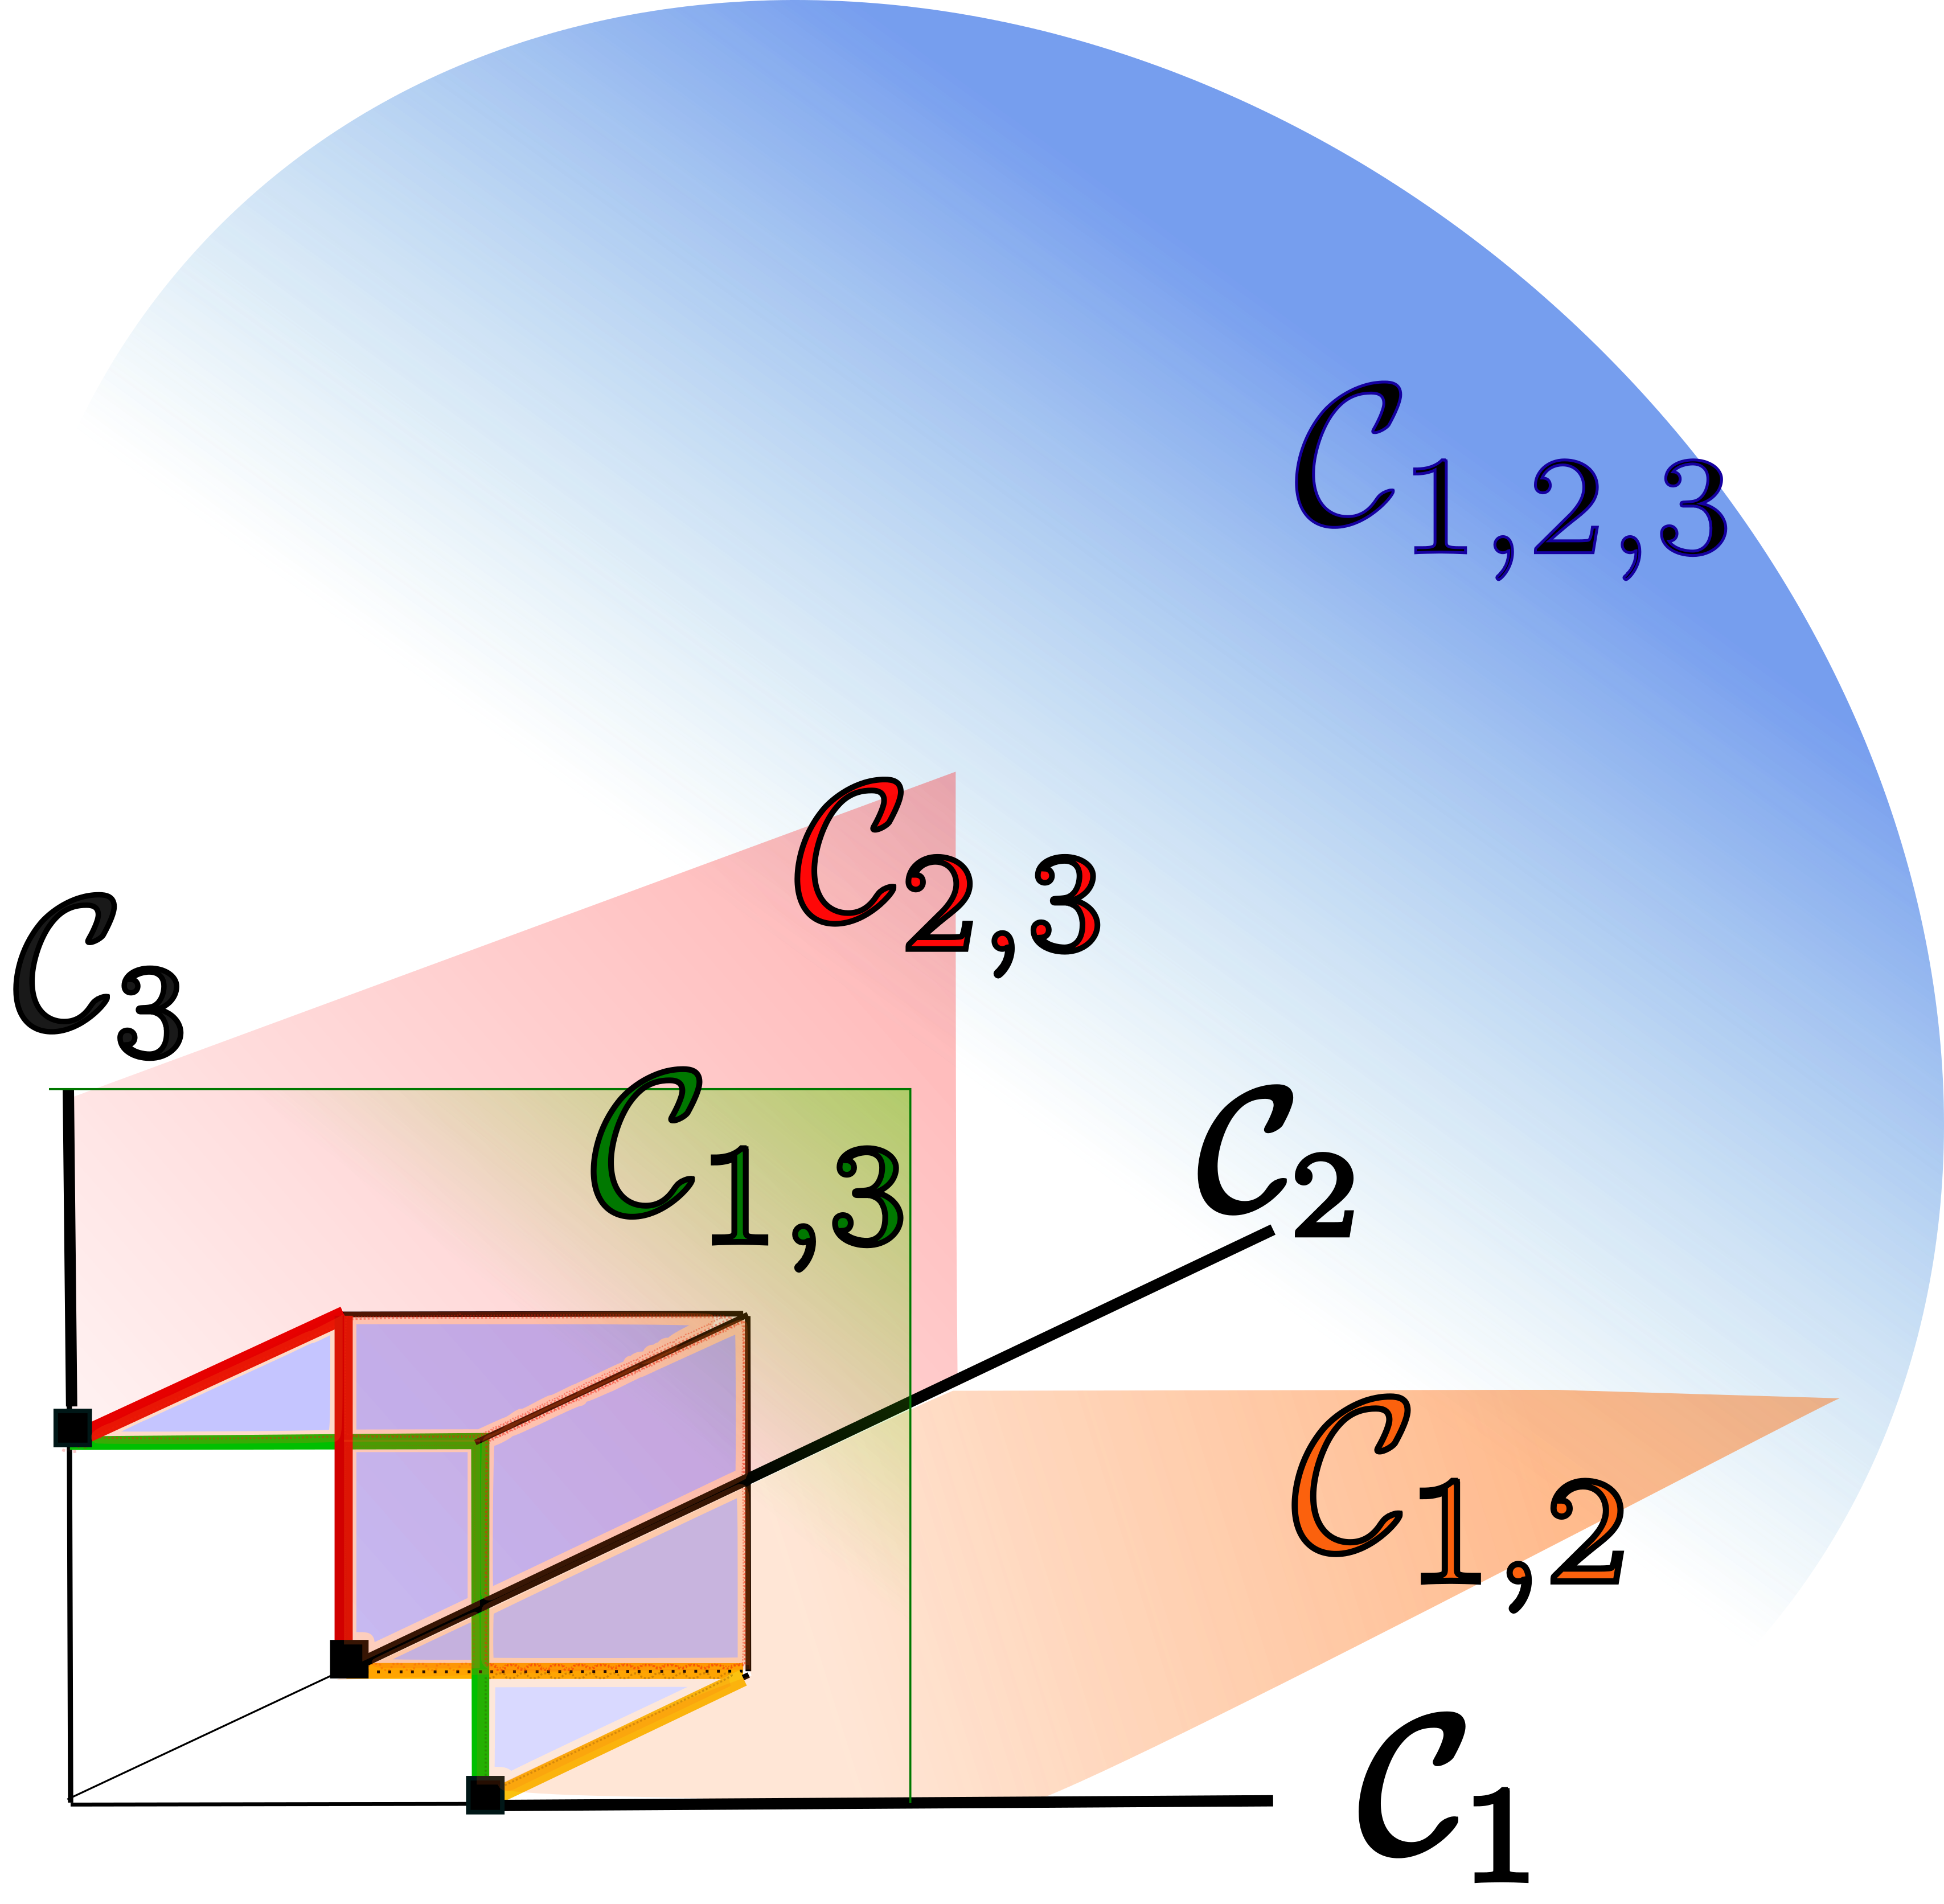
\includegraphics[scale=0.2]{fig_source/cone}
\captionof{figure}{Truncated cones in 3D}
\label{jmva:fig:3Dcones}
\end{minipage}\hfill
\begin{minipage}{0.5\linewidth}
\centering
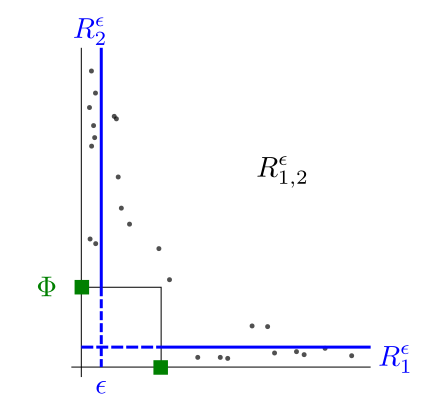
\includegraphics[width=0.64\linewidth]{fig_source/representation2D}
\captionof{figure}{Truncated $\epsilon$-rectangles in 2D}
\label{jmva:2Dcones}
\end{minipage}


\begin{lemma}\label{jmva:lem:limit_muCalphaEps}
For any non empty index subset $\emptyset \neq \alpha\subset\{1,\ldots,d\}$, the exponent measure of
$\cone_\alpha$ is
\[
\mu(\cone_\alpha) = \lim_{\epsilon\to 0} \mu(R_\alpha^\epsilon).
\]
\end{lemma}
\begin{proof}
First consider the case $\alpha=\dd$. Then $R_\alpha^\epsilon$'s forms an increasing sequence of sets as $\epsilon$ decreases and $\mathcal{C}_\alpha = R_\alpha^0 = \cup_{\epsilon>0, \epsilon \in \mathbb{Q}}~R_\alpha^\epsilon$. The result follows from the `continuity from below' property of the measure $\mu$. 
Now, for $\epsilon\ge 0$ and $\alpha\subsetneq\{1,\; \ldots,\; d\}$, consider the sets
\begin{align}
O_\alpha^\epsilon &  =\{ \mb x \in\rset_+^d~: \forall j \in \alpha:x_j > \epsilon \},  \nonumber \\
N_\alpha^\epsilon &  =\{\mb x \in\rset_+^d~: \forall j \in \alpha:   x_j > \epsilon, \exists j \notin\alpha: x_j > \epsilon \}, \nonumber
\end{align}
so that $N_\alpha^\epsilon \subset O_\alpha^\epsilon$ and $R_\alpha^\epsilon  = O_\alpha^\epsilon \setminus N_\alpha^\epsilon$. Observe also that $\cone_\alpha = O_\alpha^0\setminus N_\alpha^0$. Thus, $\mu(R_\alpha^\epsilon) = \mu(O_\alpha^\epsilon) - \mu(N_\alpha^\epsilon)$, and $\mu(\cone_\alpha) = \mu(O_\alpha^0) - \mu(N_\alpha^0)$,  so that it is sufficient to show that 
\begin{align}
\mu(N_\alpha^0) = \lim_{\epsilon\to 0}\mu(N_\alpha^\epsilon) ,
\quad \text{and}  \quad
\mu(O_\alpha^0) = \lim_{\epsilon\to 0}\mu(O_\alpha^\epsilon). \nonumber
\end{align}
Notice that the $N_\alpha^\epsilon$'s and the $O_\alpha^\epsilon$'s form two increasing sequences of sets (when $\epsilon$ decreases), and that  $N_\alpha^0 = \bigcup_{\epsilon>0,\epsilon\in\mathbb{Q}} N_\alpha^\epsilon$, $O_\alpha^0 = \bigcup_{\epsilon>0,\epsilon\in\mathbb{Q}} O_\alpha^\epsilon$. This proves the desired result.
\end{proof}


%Equipped with Lemma~\ref{jmva:lem:limit_muCalphaEps}, 

We may now  make precise the  above heuristic
interpretation of the quantities $\mu(\cone_\alpha)$: the vector
$\mathcal{M}=\{ \mu(\mathcal{C}_{\alpha}):\; \emptyset \neq
\alpha\subset\{1,\; \ldots,\; d \}\}$ asymptotically describes the
dependence structure of the extremal observations. 
% Equipped with Lemma~\ref{jmva:lem:limit_muCalphaEps}, the meaning of the
% statement 
% `$\mu(\cone_\alpha) > 0$' becomes clear. 
%
% Indeed, since the
% boundaries of the sets $\Omega_\alpha^\epsilon$ (viewed as subsets of
% $\mathbb{S}_\infty^{d-1}$) are disjoint, only a countable number of them may be
% discontinuity sets of $\Phi$. Thus, by homogeneity, the 
%  number of the sets $\cone_\alpha^\epsilon$ which are discontinuity
% sets of $\mu$ is at most countable. Hence, the threshold $\epsilon$ may be chosen arbitrarily small (so that, by
% Lemma~\ref{jmva:lem:limit_muCalphaEps}, $\mu(\cone_\alpha^\epsilon)$ is
% arbitrarily close to $\mu(\cone_\alpha)$), in such a way that
% $\cone_\alpha^\epsilon$ is a continuity set of $\mu$, 
Indeed, by
Lemma~\ref{jmva:lem:limit_muCalphaEps}, and the discussion above, $
\epsilon$ may be chosen such that $R_\alpha^\epsilon$ is a
continuity set of $\mu$, while $\mu(R_\alpha^\epsilon)$ is
arbitrarily close to $\mu(\cone_\alpha)$.  Then, using the
characterization (\ref{jmva:eq:regularVariation}) of  $\mu$, 
the following asymptotic identity  holds true:
\begin{align}
\lim_{t\to\infty} t \PP\left( \|\mb V\|_\infty\ge t, V^j> \epsilon t~~ (j \in\alpha), V^j \le \epsilon t~~ (j\notin\alpha)\right) &=\mu(R_\alpha^\epsilon) \\ \nonumber
 &\simeq \mu(\cone_\alpha). \nonumber
\end{align}
\begin{remark}
  \label{jmva:rk_approx_mu_n}
In terms of conditional probabilities, denoting $R = \|T(\mb X)\|$, where
  $T$ is the standardization map $\mb X\mapsto \mb V$,  we have
\begin{align}
\nonumber  \PP(T(\mb X)\in r R_\alpha^\epsilon~|~ R>r) = 
\frac{r \PP(\mb V\in r R_\alpha^\epsilon)}{ r\PP(\mb V \in r([\mb 0,\mathbf{1}]^c)} \xrightarrow[r\to\infty]{}\frac{\mu(R_\alpha^\epsilon)}{\mu([\mb 0,\mathbf{1}]^c)},
\end{align}
 as in~\eqref{jmva:eq:limitConditAngle}. In other terms, 
\begin{align}
\PP\left( V^j> \epsilon r~~ (j \in\alpha), V^j \le \epsilon r~~ (j\notin\alpha) ~\big\vert~ \|\mb V\|_\infty\ge r \right) &\xrightarrow[r\to\infty]{} C \mu(R_\alpha^\epsilon) \\ \nonumber
&~~~~~\simeq C\mu(\cone_\alpha), \nonumber
\end{align}
where $C = 1/ \Phi(S_\infty^{d-1}) =1/\mu([\mb 0,\mathbf{1}]^c) $.
This clarifies the meaning of `large' and `small' in the heuristic
explanation given above. 
\end{remark}

\noindent {\bf Problem statement.} % The goal of this paper is to estimate the dependence structure of the $d$-dimensional heavy-tailed r.v. $X$ in extreme
% regions from i.i.d. observations.
As explained above, our goal is to  describe the dependence on extreme
regions by investigating the structure of $\mu$ (or, equivalently,
that of $\Phi$). % , which is determined
% by that of the spectral measure $\Phi$.
More precisely, the aim is twofold. First, recover a rough
approximation of the support of $\Phi$ based on the partition
$\{\Omega_\alpha, \alpha\subset\{1,\ldots,d\}, \alpha\neq
\emptyset\}$, that is, determine which $\Omega_\alpha$'s have
nonzero mass, or equivalently, which $\mu_\alpha's$ (\emph{resp.}
$\Phi_\alpha$'s) are nonzero. This support estimation is potentially
sparse (if a small number of $\Omega_\alpha$ have non-zero mass) and
possibly low-dimensional (if the dimension of the sub-cones
$\Omega_\alpha$ with non-zero mass is low).
%a well chosen partition of the input space, 
The second objective is to 
investigate how the exponent measure $\mu$ spreads its mass on the
$\mathcal{C}_{\alpha}$'s, the theoretical quantity
$\mu(\mathcal{C}_{\alpha})$ indicating to which extent extreme
observations may occur in the `direction' $\alpha$ for $\emptyset
\neq \alpha \subset \{1,\; \ldots,\; d \}$. 
%  estimate the amount of angular mass
% $\mu(\cone_\alpha) = \Phi(\Omega_\alpha)$  on each non-void element of the
% partition.
These two goals are achieved using empirical versions of
the angular measure defined in
Section~\ref{jmva:sec:classicEstimators}, evaluated on the
$\epsilon$-thickened rectangles $R_\alpha^\epsilon$.
% This problem can be tackled by investigating how the exponent measure
% $\mu$ spreads its mass on the $\mathcal{C}_{\alpha}$'s, the
% theoretical quantity $\mu(\mathcal{C}_{\alpha})$ indicating to which
% extent extreme observations may occur in the `direction' $\alpha$ for
% $\emptyset \subsetneq \alpha \subset \{1,\; \ldots,\; d \}$.
Formally, we wish to recover the $(2^{d}-1)$-dimensional unknown
vector 
\begin{align}
\label{jmva:eq:representation_M}
\mathcal{M}=\{ \mu(\mathcal{C}_{\alpha}):\; \emptyset \neq \alpha\subset\{1,\; \ldots,\; d \}\}
\end{align}
 from $\mb X_1,\;
\ldots,\; \mb X_n\overset{i.i.d.}{\sim} \mb F$ and build an estimator
$\widehat{\mathcal{M}}$ such that
\begin{align}
\nonumber
\vert\vert \widehat{\mathcal{M}} -\mathcal{M}
\vert\vert_{\infty} \;%\overset{def}
{=} \; \sup_{\emptyset \neq \alpha \subset \{1,\; \ldots,\; d \}}\; \vert
\widehat{\mathcal{M}}(\alpha)- \mu(\mathcal{C}_{\alpha})\vert
\end{align}
is small with large probability.  % As $\mu(\mathcal{C}_{\alpha})=\Phi(\Omega_{\alpha})$ for any $\alpha$ and
In view of Lemma~\ref{jmva:lem:limit_muCalphaEps}, (biased) estimates of
$\mathcal{M}$'s components are built from an empirical version of 
the exponent measure, evaluated on the
$\epsilon$-thickened rectangles $R_\alpha^\epsilon$ (see Section~\ref{jmva:sec:classicEstimators} below). As a by-product, one obtains an estimate of the support of the limit measure $\mu$,
\begin{align}
\bigcup_{\alpha:\; \widehat{\mathcal{M}}(\alpha)>0 }\mathcal{C}_{\alpha}. \nonumber
\end{align}
 The results stated in the next section are non-asymptotic and sharp bounds are given by means of {\sc VC} inequalities tailored to low probability regions.
%, which is determined
%by that of the spectral measure $\Phi$. 
%More precisely,  the aim is
%twofold: first, recover a rough approximation of the support of
%$\Phi$ based on  the partition $\{\Omega_\alpha,
%\alpha\subset\{1,\ldots,d\}, \alpha\neq \emptyset\}$, that is,
%determine which $\Omega_\alpha$'s have nonzero mass, or equivalently,
%which $\mu_\alpha's$ (\emph{resp.} $\Phi_\alpha$'s) are nonzero; 
%a well chosen partition of the input space, 
%second, estimate the amount of angular mass
%$\mu(\cone_\alpha) = \Phi(\Omega_\alpha)$  on each non-void element of the
%partition.  These two goals are achieved using empirical versions of
%the angular measure defined in
%section~\ref{jmva:sec:nonParamEstimators}, evaluated on the
%$\epsilon$-thickened cones $\cone_\alpha^\epsilon$. Non-asymptoitc upper bounds on 
%the error are derived in section~\ref{jmva:sec:estimation} using VC
%inequalities adapted to low probability regions. 


\subsection{Regularity Assumptions}\label{jmva:sec:RegularAssumptions} % and Further Notations}
Beyond the existence of the limit measure $\mu$ (\ie~multivariate regular variation of $\mathbf{V}$'s distribution, see~\eqref{jmva:intro:regvar}), and thus, existence of an angular measure $\Phi$ (see (\ref{jmva:mu-phi})),
three additional assumptions are made, which are natural when estimation of the support of a distribution is considered. 

\begin{assumption}\label{jmva:hypo:continuous_margins}
The margins of $\mb X$ have continuous c.d.f., namely $F_j,~1 \le j \le d$ is continuous.
\end{assumption}
\noindent
 Assumption~\ref{jmva:hypo:continuous_margins}
is widely used in the context of non-parametric estimation of the dependence
structure (see \emph{e.g.} \cite{Einmahl2009}): it ensures that the transformed variables $V^j = (1 -
F_j(X^j))^{-1}$ (\emph{resp.} $U^j =  1 -F_j(X^j)$) have indeed a
standard Pareto distribution, $\P(V^j>x) = 1/x,~ x\ge 1$ (\emph{resp.}
the $U^j$'s are uniform variables). 

\bigskip
For any non empty subset $\alpha$ of $\{1,\; \ldots,\;d\}$, one denotes by $\ud x_\alpha$ the Lebesgue measure on ${\cal C}_\alpha$ and write $\ud x_\alpha  = \ud x_{i_1}\ldots\ud x_{i_k}$, when $\alpha=\{i_1, \ldots , i_k\}$. For convenience, we also write $\ud x_{\alpha\setminus{i}}$ instead of  $\ud x_{\alpha\setminus{\{i\}}}$.
% \begin{align*}
%   \mathcal{C}_\alpha^\epsilon = \{  \|x\| \ge 1: &\frac{x_i}{\|x\|_\infty} > \epsilon \text{ for }
%   i\in\alpha, \\
% &\frac{x_i}{\|x\|_\infty}\le\epsilon \text{ for } i\notin \alpha \quad \}~.
% \end{align*}
\begin{assumption}\label{jmva:hypo:continuousMu}
Each component $\mu_\alpha$ of~\eqref{jmva:eq:decomp1} is absolutely continuous w.r.t.
Lebesgue measure $\ud x_\alpha$ on ${\cal C}_\alpha$. %This implies that $\Phi_\alpha$ is absolutely continuous with respect to the Lebesgue measure on $\Omega_\alpha$. It is also assumed that, each of the induced densities is bounded.
\end{assumption}
\noindent
% For $\alpha\subset \{1,\ldots ,d\}$,  $\alpha\neq
% \emptyset$, the subset of the sphere corresponding to the cones is
% \begin{align*}
% \Omega_{\alpha} & = \{x \in S_{\infty}^{d-1} :  x_i > 0 \text{ for } i\in\alpha~,~  x_i = 0 \text{ for } i\notin \alpha   \} \\
% & = S_{\infty}^{d-1}\cap {\mathcal{C}}_\alpha ~ .
% \end{align*}
% \noindent
% Thus, the $\Omega_\alpha $'s form  a partition of $S_\infty^{d-1}$, and we have 
% \begin{align*}
% \mu(\mathcal{C}_i) ~=~  \Phi(\Omega_i) \text{ ~~~and~~~ } \Phi ~=~ \sum_{\emptyset \subsetneq \alpha\subset\{1,\ldots ,d\}} \Phi_\alpha ~,
% \end{align*}  
% \noindent
% where $\Phi_\alpha$ denotes the restriction of $\Phi$ to $S_{\infty}^{d-1} \cap {\Omega}_\alpha$.
Assumption~\ref{jmva:hypo:continuousMu} has a very convenient consequence 
regarding $ \Phi$: the fact that the exponent measure $\mu$ spreads no mass on subsets of the form 
$\{\mb x: \;\ninf{\mb x} \ge 1, x_{i_1} = \dotsb =  x_{i_r} \neq 0 \}$ with $r \ge 2$,
implies that the spectral measure $\Phi$ spreads no mass on edges $\{\mb x: \;\ninf{\mb x} = 1,  \; x_{i_1} = \dotsb =  x_{i_r} =1 \}$ with $r \ge 2~.$
This is summarized by the following result.
\begin{lemma}\label{jmva:lem:continuousPhi}
Under Assumption~\ref{jmva:hypo:continuousMu}, the following assertions holds true.
\begin{itemize}
\item  $ \Phi$ is concentrated on the (disjoint) edges
\begin{align}
   \Omega_{\alpha,i_0} = \{\mb x: \; \ninf{\mb x}  = 1,\; x_{i_0} = 1,~~& 0<  x_i < 1 ~~\text{~for~} i \in \alpha \setminus \{i_0\}\\ \nonumber
&x_i=0 ~~~~\text{~~~ for } i\notin \alpha ~~~~~~~\} \nonumber
\end{align}
for $i_0\in\alpha$, $\emptyset \neq \alpha\subset\{1,\; \ldots,\; d \}$.
\item The restriction $\Phi_{\alpha,i_0}$ of $\Phi$ to
  $\Omega_{\alpha,i_0}$ is absolutely continuous \wrt~the Lebesgue measure $\ud x_{\alpha\setminus{i_0}}$ on the cube's edges, whenever $|\alpha|\ge 2 $.

\end{itemize}
\end{lemma}
\begin{proof}
  The first assertion straightforwardly results from the discussion above.  Turning to the
  second point, consider any  measurable
  set $D \subset \Omega_{\alpha,i_0}$ such that $\int_{D}\ud x_{\alpha \setminus i_0} = 0$. Then the
  induced truncated cone $\tilde D = \{ \mb v:~ \|\mb v\|_\infty \ge
  1, \mb v / \|\mb v\|_\infty \in D \}$ satisfies $\int_{\tilde D}\ud
  x_{\alpha} = 0$ and belongs to $\mathcal{C}_\alpha$. Thus,  by virtue of
  Assumption~\ref{jmva:hypo:continuousMu}, $\Phi_{\alpha,
    i_0}(D)=\Phi_{\alpha}(D) = \mu_\alpha(\tilde D) = 0$.
\end{proof}

\noindent
It follows from Lemma~\ref{jmva:lem:continuousPhi} that the angular
measure $\Phi$ decomposes as $\Phi = \sum_{\alpha} \sum_{i_0\in\alpha}
\Phi_{\alpha,i_0}$  and that there exist densities $ \frac{\ud
  \Phi_{\alpha,i_0}}{\ud x_{ \alpha \smallsetminus i_0}},~~
|\alpha|\ge 2,~i_0\in\alpha,$ such that for all $B \subset
\Omega_\alpha,~~ |\alpha| \ge 2$,
\begin{align}
\label{jmva:eq:decomposePhi}
\Phi(B)~=~ \Phi_\alpha(B)~=~ \sum_{i_0\in\alpha} \int_{B\cap \Omega_{
    \alpha,i_0} } \frac{\ud \Phi_{\alpha,i_0}}{\ud x_{ \alpha
    \smallsetminus i_0}}(x) \ud x_{\alpha\setminus i_0}. 
\end{align}
% In view of equation~\eqref{jmva:eq:decomposePhi},  in particular, 
% \begin{lemma}
% Each $\Phi_{\alpha,i_0}$ is continuous with respect to $\ud x_i$, for
% $i\in\alpha \setminus \{i_0\}$ .
% \end{lemma}
In order to formulate the next assumption, for $|\beta| \ge 2$, we set
\begin{align}
\label{jmva:eq:supDensity}
M_\beta = % \sup_{i,j \in\beta,~ j\neq i} ~~~~\sup_{x\in\Omega_{\beta,i}} ~~~~ \frac{\ud  \Phi_{\beta, i}}{\ud x_j}(x)  ~~??=??~
~ \sup_{i \in\beta} ~~\sup_{x\in\Omega_{\beta,i}} ~~~~ \frac{\ud  \Phi_{\beta, i}}{\ud x_{\beta \setminus i}}(x).
\end{align}


\begin{assumption}\label{jmva:hypo:abs_continuousPhi}({\sc Sparse Support})
  The angular density is uniformly bounded on $S^{d-1}_\infty$ ($\forall |\beta| \ge 2,~M_\beta < \infty$), and there exists a constant  $M>0$, such that we have $\sum_{|\beta| \ge 2} M_\beta < M$, where the sum is over subsets $\beta$ of $\{1,\ldots,d\}$ which contain at least two elements.
\end{assumption}

\begin{remark}
The constant $M$ is problem dependent. However, in the case where our representation $\mathcal{M}$ defined in \eqref{jmva:eq:representation_M} is the most informative about the angular measure, that is, when the density of $\Phi_\alpha$ is constant on $\Omega_\alpha$, we have $M \le d$: Indeed, in such a case, 
$M \le \sum_{|\beta| \ge 2} M_\beta |\beta| = \sum_{|\beta| \ge 2} \Phi(\Omega_\beta) \le \sum_\beta \Phi(\Omega_\beta) \le \mu([\mb 0,\mb 1]^c)$.
% An order of magnitude for the value of $M$ is given as follows. Assuming that $\Phi$ has constant density on each sub-sphere $\Omega_\alpha$, then
% $\mu([\mb 0,\mb 1]^c) = \sum_\beta \Phi(\Omega_\beta) \ge \sum_{|\beta| \ge 2} \Phi(\Omega_\beta) = \sum_{|\beta| \ge 2} M_\beta |\beta| $.
The equality inside the last expression comes from the fact that the Lebesgue measure of a sub-sphere $\Omega_\alpha$ is $|\alpha|$, for $|\alpha| \ge 2$. Indeed, using the notations defined in Lemma~\ref{jmva:lem:continuousPhi}, $\Omega_\alpha = \bigsqcup_{i_0 \in \alpha}\Omega_{\alpha,i_0}$, each of the edges $\Omega_{\alpha,i_0}$ being unit hypercube. % (Intuitively, in dimension 3, $\Omega_{\{1,2,3\}}$ is a cube whose 3 faces corresponding to the positive quadrant are unit squares).
Now, $\mu([\mb 0,\mb 1]^c) \le \mu(\{v,~ \exists j,~ v_j > 1\} \le d \mu(\{v,~v_1 >1\})) \le d$.
% Noting that the Lebesgue measure of a sub-sphere $\Omega_\alpha$ is $|\alpha|$, if $\Phi$ is constant on each sub-sphere we have
% $\mu([\mb 0,\mb 1]^c) = \sum_\beta \Phi(\Omega_\beta) \ge \sum_{|\beta| \ge 2} \Phi(\Omega_\beta) = \sum_{|\beta| \ge 2} M_\beta |\beta| $

\noindent
Note that the summation $\sum_{|\beta| \ge 2} M_\beta |\beta|$ is smaller than $d$ despite the (potentially large) factors $|\beta|$. Considering $\sum_{|\beta| \ge 2} M_\beta$ is thus reasonable: in particular, $M$ will be small when only few $\Omega_\alpha$'s have non-zero $\Phi$-mass, namely when the representation vector $\mathcal{M}$ defined in \eqref{jmva:eq:representation_M} is sparse.
\end{remark}
\noindent Assumption~\ref{jmva:hypo:abs_continuousPhi} is naturally involved in the derivation of upper bounds on the error made when approximating $\mu(\cone_\alpha)$ by the empirical counterpart of $\mu(R_\alpha^\epsilon)$.
The estimation error bound derived in Section~\ref{jmva:sec:estimation} depends on the sparsity constant $M$.

%XXX commments on these assumptions
% \begin{assumption}\label{jmva:hypo:M}
% For every $\beta$ such that $|\beta| > 2$,~ $M_\beta$ is finite and $|\beta_1| \le |\beta_2| \Rightarrow M_{\beta_1} \ge M_{\beta_2}$.
% \end{assumption}
% One 'parcimony assumption' would be something like $M_\beta\le e^{-|\beta|}$.

% In other words we select, for each feature $j\le d$, the `$k$ largest values' $X_i^j$
% over the $n$ observations. According to the nature of the extremal dependence,
% a number between $k$ and $dk$ of observations are selected: $k$ in
% case of perfect dependence, $dk$ in case of `asymptotic independence', which
% means, in EVT, that the components may only be large one at a time. In
% any case, the number of observations considered as extreme is proportionnal to $k$, whence the normalizing factor $\frac{n}{k}$. 

%


% Yet the goal is to study the dependence between the $V_i^j$, $i$ fixed anf $j$ varying.
% One way to proceed is to characterize, for each subset of features
% $\alpha \subset \{1,...,d\}$, the `correlation' of these features
% given that one of them at least  is large and the others are small. %extreme (\ie~given that the observation is extreme).
% Formally, we  associate to each such $\alpha$ a coefficient
% $\mu_n^\alpha$ reflecting the degree of dependence between the
% features $\alpha$. Theoretically, by definition of asymptotic
% dependence, this coeficient is to be proportional to the expected number of
% points $V$ verifying $V^j > 0$, $j \in \alpha$ and $V^j = 0,~ j\notin
% \alpha$, and $\|V\|_\infty\ge r$, namely $ r^{-1}V \in \mathcal{C}_\alpha$ with 
% \begin{align}
% %\label{jmva:cone}
% \mathcal{C}_\alpha = \{v \ge 0,~\|v\|_\infty \ge 1,~ v_j > 0 ~\text{ for } j \in \alpha,~ v_j = 0 ~\text{ for } j \notin \alpha \}.
% \end{align}
% (see Fig.~\ref{jmva:fig:3Dcones}) But in practice, the data are non-asymptotic so that if $\alpha \neq \{1,\ldots,d\}$ the cones $\mathcal{C}_\alpha$ have zero Lebesgue measure and are not likely to receive empirical mass. Consider then a tolerance parameter $\epsilon>0$ and approximate the asymptotic mass of $~\mathcal{C}_\alpha~$ by the non-asymptotic mass of 
% \begin{align}
%  \label{jmva:eq:epsilonCone}
%  ~\mathcal{C}_\alpha^\epsilon~=\{v \ge
%  0,~\|v\|_\infty \ge 1,~ v_j > \epsilon \|v\|_\infty ~\text{ for } j
%  \in \alpha,~v_j \le \epsilon\|v\|_\infty ~\text{ for } j \notin \alpha
%  \} ,
% \end{align}
% which leads to coefficients 

% This motivates the study of the \stdf $l$, since it is now theoretically clear how the asymptotic tail dependence structure of $F$ is contained in $l$.
% XXXXXXXXXXXXXXXXXXXXXXXXXXXXXXXXXXXXXXXXXXXXXXXXXXXXXXXXXXXXXXXXXXXXXXXXXXXXXXXXXXXXXXXXXXXXXXXX
% % The measures $\mu$ and $\Lambda$ are called exponent measures and have the following properties:
% % \begin{itemize}
% % \item standardized marginals: for all $a>0$,
% % \begin{align*}
% % \Lambda([0,a]\times[0,\infty]^{d-1})~=~\Lambda([0,\infty]&\times[0,a]\times[0,\infty]^{d-2})
% % \\&~=~...~=~\Lambda([0,\infty]^{d-1}\times[0,a])~=~a
% % \end{align*}
% % \noindent and
% % \begin{align*} 
% % \mu([a,\infty]\times[0,\infty]^{d-1})~=~\mu([0,\infty]&\times[a,\infty]\times[0,\infty]^{d-2})
% % \\&~=~...~=~\mu([0,\infty]^{d-1}\times[a,\infty])~=~a^{-1}
% % \end{align*}
% % \item homogeneity: $\Lambda(c.)=c~ \Lambda(.)$ and $\mu(c.)=c^{-1} \mu(.)$
% % \item concentration: $\Lambda$, $\mu$ are respectively concentrated on $(0,\infty]^d \setminus \{\infty\}$, $[0,\infty)^d \setminus \{0\}$
% % \end{itemize}
% The homogeneity property yields a decomposition of $\mu$ into a
% radial and angular part (see de Haan and Resnick ...). 

\section{A non-parametric estimator of the subcones' mass : definition and preliminary results}
\label{jmva:sec:estimation}

In this section, an estimator $\widehat{\mathcal{M}}(\alpha)$ of each of the sub-cones' mass
$\mu(\cone_\alpha)$, $\emptyset\neq\alpha\subset\dd$, is
  proposed, based on observations  $\mb X_1,.\ldots, \mb X_n$, \iid~copies of $\mb X\sim \mb F$.
Bounds on the error $\vert\vert
  \widehat{\mathcal{M}}-\mathcal{M}\vert\vert_{\infty}$ are
  established. In the remaining of this chapter, we work under
  Assumption~\ref{jmva:hypo:continuous_margins} (continuous margins, see
  Section~\ref{jmva:sec:RegularAssumptions}). 
Assumptions~\ref{jmva:hypo:continuousMu}~and~\ref{jmva:hypo:abs_continuousPhi}
are not necessary to prove a preliminary result on a class of
rectangles (Proposition~\ref{jmva:prop:g} and Corollary~\ref{jmva:cor:mu_n-mu}). However, they are required % to approximate cones with rectangles
% (Proposition~\ref{jmva:prop:mu_n-mu}) and
to bound the bias induced by the tolerance parameter
$\epsilon$ (in Lemma~\ref{jmva:lemma_simplex}, Proposition~\ref{jmva:prop_simplex} and in the main result, Theorem~\ref{jmva:thm-princ}).  
% under the hypotheses listed in Section~\ref{jmva:sec:RegularAssumptions}. %  , we next investigate the problem of estimating $\mathcal{M}$ based on observations  $\mb X_1,.\ldots, \mb X_n$, \iid copies of $\mb
% % X\sim F$.
\subsection{A natural empirical version of the exponent measure mu}
\label{jmva:sec:classicEstimators}
 Since the marginal distributions $F_j$ are unknown, we classically consider
the empirical counterparts of the $\mb V_i$'s, 
$\mb{\widehat  V}_i = (\widehat V_i^1, \ldots,\widehat
V_i^d)$, $1\le i\le n$, as standardized  variables obtained from a
rank transformation (instead of a probability integral
transformation),  
\[\mb{\widehat  V}_i = \left( ( 1- \widehat F_j
  (X_i^j))^{-1}\right)_{1 \le j \le d}~, \]
  where 
$\widehat F_j (x) = (1/n) \sum_{i=1}^n \mathbf{1}_{\{X_i^j < x\}}$.
%
We denote by $T$ (\emph{resp.} $\widehat T$) the standardization
(\textit{resp.} the empirical standardization), 
\begin{align}
\label{jmva:def:transform}
T(\mb x) = \left( \frac{1}{1- F_j (x^j)}\right)_{1\leq j\leq d}
\text{~~and~~}
\widehat T(\mb x) = \left( \frac{1}{1- \widehat F_j(x^j)}\right)_{1\leq j\leq d}. 
\end{align}
The empirical probability distribution of the rank-transformed data is then given by
\begin{align*}
\mathbb{\widehat P}_n=(1/n)\sum_{i=1}^n\delta_{\mb{\widehat{V}}_i}.
\end{align*}
Since for a $\mu$-continuity set $A$ bounded away from $0$,   $t~ \mathbb{P}\left( \mb V \in t A\right)  \to \mu(A)$ as $t \to \infty$, see~\eqref{jmva:eq:regularVariation}, a natural empirical version of $\mu$ is defined as 
\begin{align}\label{jmva:mu_n}
\mu_n(A) ~=~ \frac{n}{k} \widehat{\mathbb{P}}_n (\frac{n}{k}A) ~=~ \frac{1}{k}\sum_{i=1}^n \mathbf{1}_{\{\mb{\widehat{V}}_i \in \frac{n}{k} A\}}~.
\end{align}
 Here and throughout, we place ourselves in the asymptotic setting stipulating that $k = k(n) >0$ is such that $k \to \infty$ and $k = o(n)$ as $n \to \infty$.
The ratio $n/k$ plays the role of a large radial threshold.
Note that this estimator is commonly used in the field of
non-parametric estimation of the dependence structure, see \textit{e.g.}
\cite{Einmahl2009}. 


\subsection{Accounting for the  non asymptotic nature of  data:
  epsilon-thickening.}

 Since the cones $\mathcal{C}_\alpha$ have zero Lebesgue measure, 
and since, under Assumption~\ref{jmva:hypo:continuous_margins}, the margins are
continuous, the cones  are not likely to receive any empirical mass, 
 so that  simply counting points in $\frac{n}{k}\mathcal{C}_\alpha$ is not an
option: with probability one, only
the largest dimensional cone (the central one, corresponding to
$\alpha= \{1,\ldots,d\})$ will be hit. 
%
In view of Subsection~\ref{jmva:sec:decomposMu} and
Lemma~\ref{jmva:lem:limit_muCalphaEps}, 
 it is natural to introduce a 
tolerance parameter $\epsilon>0$ and to approximate the asymptotic mass
of $\mathcal{C}_\alpha$ with the non-asymptotic mass of
$R_\alpha^\epsilon$. We thus define the non-parametric estimator $\widehat{M}(\alpha)$ of
$\mu(\cone_\alpha)$ as
\begin{align}
\label{jmva:heuristic_mu_n}
\hatmass(\alpha) = \mu_n(R_\alpha^\epsilon), \qquad
\emptyset\neq\alpha\subset\dd.  %= \frac{n}{k} \mathbb{\hat P}_n \left ( \frac{n}{k} \mathcal{C}_\alpha^\epsilon \right),
\end{align}
%where $\mathbb{\hat P}_n=(1/n)\sum_{i=1}^n\delta_{\hat{V}_i}$ is the empirical probability distribution of the rank-transformed data.
Evaluating  $\hatmass(\alpha)$  boils down (see~\eqref{jmva:mu_n})
to counting points in $(n/k)\,R_{\alpha}^{\epsilon}$, as illustrated in Figure~\ref{jmva:estimation_rect}. The estimate $\hatmass(\alpha)$ is thus a (voluntarily
$\epsilon$-biased) natural estimator of $\Phi(\Omega_\alpha) = \mu(\mathcal{C}_\alpha)$.
\begin{figure}[!ht]
  \centering
  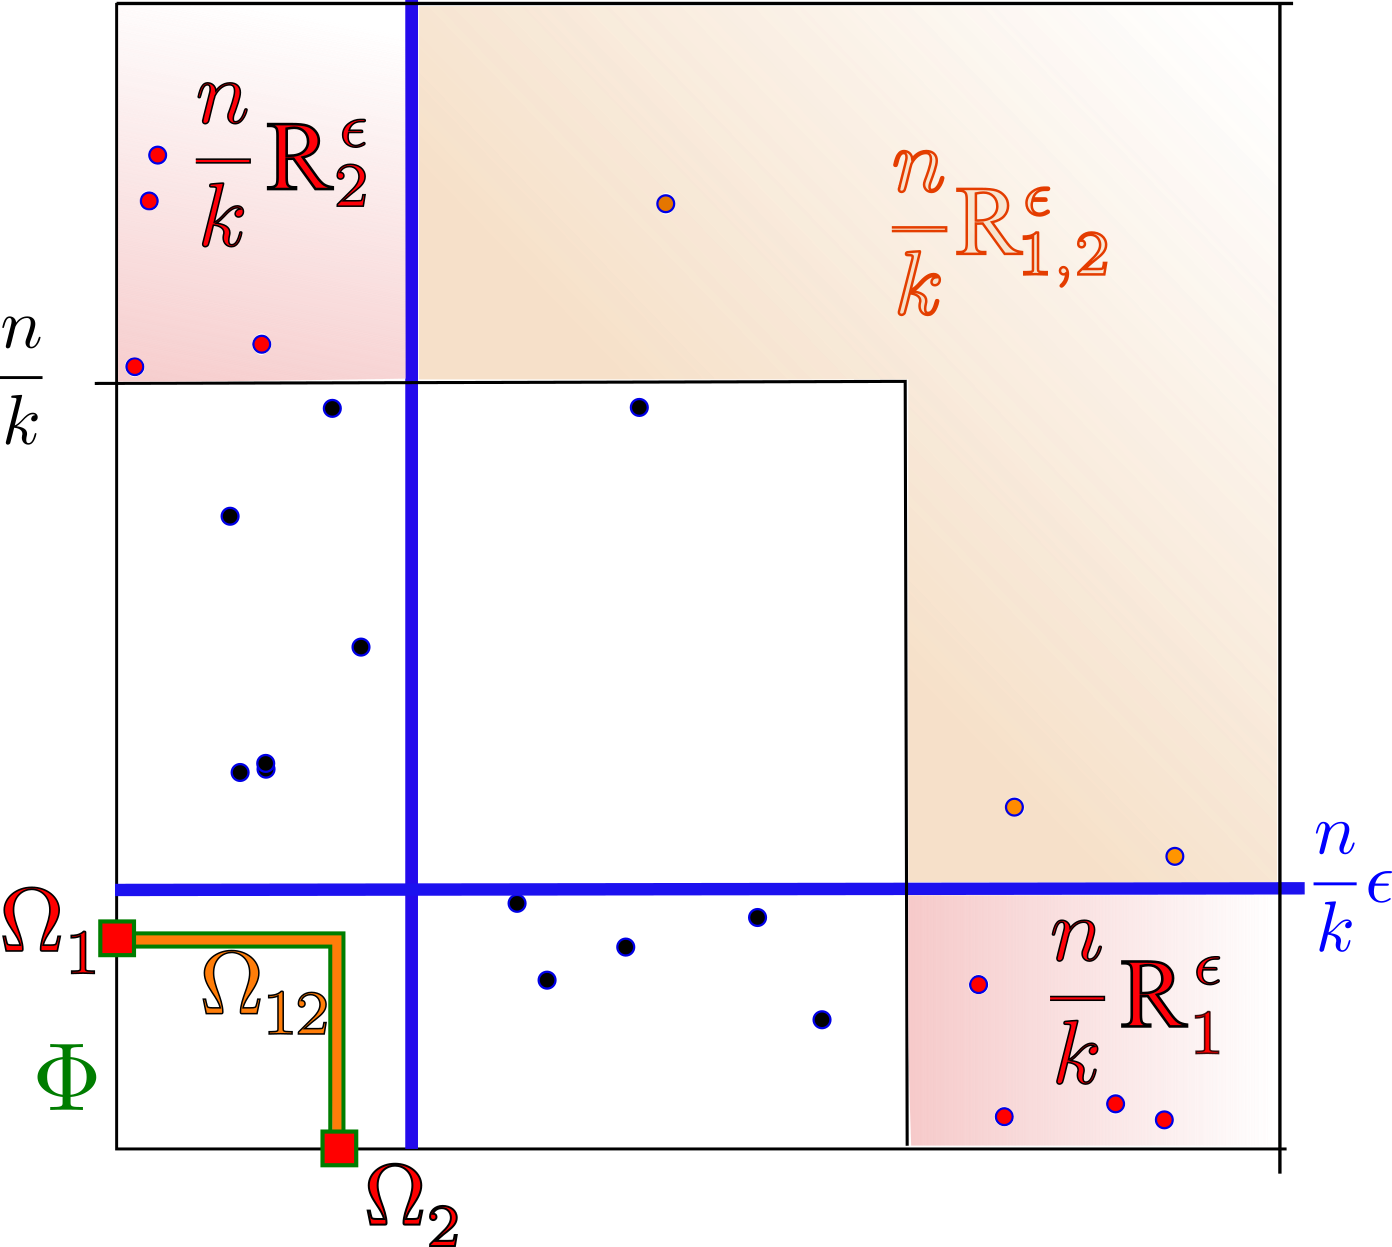
\includegraphics[width = 0.7\textwidth]{fig_source/representation2D_nk_rect.png}
  \caption{Estimation procedure}
  \label{jmva:estimation_rect}
\end{figure}


The coefficients $(\hatmass(\alpha))_{\alpha\subset\{1,\ldots,d\}}$ related to the cones $\mathcal{C}_\alpha$ constitute a summary representation of the dependence structure.  % constitute a   A representation of the dependence structure is then
% \begin{align}
% R_n(x) = \sum_{\alpha }\hatmass(\alpha) \mathds{1}_{\hat T(x) \in \mathcal{C}_\alpha^\epsilon},
% \end{align}
This representation is sparse as soon as the $\mu_n^{\alpha,  \epsilon}$ are positive only for a few groups of features $\alpha$ (compared to the total number of groups or sub-cones, $2^d$ namely). It is  is low-dimensional as soon as each of these groups $\alpha$ is of small cardinality, or equivalently the corresponding sub-cones are low-dimensional compared with $d$.

In fact, $\hatmass(\alpha)$ is (up to a normalizing constant) an empirical version of the  conditional probability that $T(\mb X)$ belongs to the rectangle $ r R_\alpha^\epsilon$, given that $\|T(\mb X)\|$ exceeds  a large threshold $r$. Indeed, as explained in Remark~\ref{jmva:rk_approx_mu_n},  
\begin{align}\label{jmva:eq:interprete_mun_Pcondit}
\mathcal{M}(\alpha) = \lim_{r \to \infty} \mu([\mb 0,\mathbf{1}]^c)~~\mathbb{P}(T(\mb X)\in r R_\alpha^\epsilon ~|~ \|T(\mb X)\|\ge r) . 
\end{align}

The remaining of this section is devoted to obtaining non-asymptotic upper bounds on the error $\vert\vert \widehat{\mathcal{M}}-\mathcal{M}\vert\vert_{\infty}$. 
The main result is stated in Theorem~\ref{jmva:thm-princ}. 
Before all, notice that the error may be obviously decomposed as the sum of a stochastic term and a bias term inherent to the $\epsilon$-thickening approach:
\begin{align}
\vert\vert \widehat{\mathcal{M}}-\mathcal{M}\vert\vert_{\infty} &~=~\max_{\alpha} |
\mu_n(R_\alpha^\epsilon)-\mu(\mathcal{C}_\alpha)|\nonumber
\\&~\le~ ~\max_\alpha |\mu-\mu_n|(R_\alpha^\epsilon) ~+~ \max_\alpha|\mu(R_\alpha^\epsilon)-\mu(\mathcal{C}_\alpha)|~.\label{jmva:error_decomp} 
\end{align}
Here and beyond, to keep the notation uncluttered, we simply denotes `$\alpha$'  for `$\alpha$ non empty subset of $\{1,\; \ldots,\;d\}$'. The main steps of the argument leading to Theorem~\ref{jmva:thm-princ} are  as follows. First, obtain a uniform upper bound on the error $|\mu_n - \mu|$ restricted to a well chosen VC class of rectangles (Subsection~\ref{jmva:sec:rectangles}), and deduce an uniform bound on  $|\mu_n - \mu|(R_\alpha^\epsilon)$ (Subsection~\ref{jmva:sec:boundErrorEpsilonCones}). Finally, using the regularity assumptions (Assumption~\ref{jmva:hypo:continuousMu} and Assumption~\ref{jmva:hypo:abs_continuousPhi}), bound the difference $|\mu(R_\alpha^\epsilon) - \mu(\cone_\alpha)|$ (Subsection~\ref{jmva:sec:boundMuEpsilonCones}). 


\subsection{Preliminaries: uniform approximation over a VC-class of rectangles}
\label{jmva:sec:rectangles}
This subsection builds on the theory developed in Chapter~\ref{colt}, where a non-asymptotic bound is stated on the estimation of the stable tail dependence function (defined in~\eqref{back:stdf1}). % We prove here (Proposition~\ref{jmva:prop:g}) a generalized version of the result obtained by these authors. 
The \stdf~$l$ is related to the class of sets of the form $[\mb 0, \mb v]^c$ (or $[\mb u, \boldsymbol{\infty}]^c$ depending on which standardization is used), and an equivalent definition is 
\begin{align}
\label{jmva:stdf}
l(\mathbf{x}):= \lim_{t \to \infty} t \tilde F (t^{-1}\mathbf{x}) = \mu([\mb 0, \mb x ^{-1}]^c) 
\end{align}
\noindent
with $\tilde F (\mathbf{x}) = (1-F) \big( (1-F_1)^\leftarrow(x_1),\ldots, (1-F_d)^\leftarrow(x_d)  \big)$.
 Here the notation
$(1-F_j)^\leftarrow(x_j)$ denotes the quantity $\sup\{y\,:\; 1-F_j(y) \ge x_j\}$. Recall that the marginally uniform variable $\mb U$ is defined by  $U^j = 1-F_j(X^j)$ ($1\le j\le d$). Then  in terms of standardized variables $U^j$, 
\begin{align}
\label{jmva:def:tildeF}
\tilde F(\mb x) = \P\Big(\bigcup_{j=1}^d\{U^j< x_j\}\Big) = \P(\mb
U\in [\mb x, \boldsymbol{\infty}[^c) = \P(\mb V \in [\mb 0, \mb x^{-1}]^c). 
\end{align}

A natural estimator of $l$ is its empirical version defined as
follows,  see \cite{Huangphd}, \cite{Qi97}, \cite{Drees98}, \cite{Einmahl2006}, \cite{COLT15}:
\begin{align}\label{jmva:empir-Stdf}
l_n(\mathbf{x}) &= \frac{1}{k}~\sum_{i=1}^{n} \mathds{1}_{\{ X_i^1 \ge
  X^1_{(n-\lfloor kx_1 \rfloor+1)}  \text{~~or~~} \ldots \text{~~or~~}
  X_i^d \ge  X^d_{(n-\lfloor kx_d\rfloor+1)}  \}}~.
\end{align}
The expression is indeed suggested by the definition of $l$ in  (\ref{jmva:stdf}), with all distribution functions and  univariate quantiles replaced by their empirical counterparts, and with $t$  replaced by $n/k$.
The following lemma allows to derive alternative expressions for the empirical version of the \stdf.  
\begin{lemma}
\label{jmva:lem:equivalence}
Consider the rank transformed variables 
$\mb{  \widehat U}_i = (\mb{ \widehat V}_i)^{-1} = ( 1- \widehat F_j
(X_i^j))_{1\leq j\leq d}$ for $i = 1, \ldots, n$. Then, for $(i,j)\in \{1,\ldots, n\}\times \{1,\ldots,d\}$,
with probability one,
$$
\widehat U_i^j \le \frac{k}{n} x_j^{-1} ~\Leftrightarrow~
\widehat V_i^j \ge \frac{n}{k} x_j ~\Leftrightarrow~
X_i^j \ge X_{(n-\lfloor  kx_j^{-1} \rfloor +1)}^j ~\Leftrightarrow~
U_i^j \le U_{(\lfloor kx_j^{-1}\rfloor)}^j~.
$$
\end{lemma}
The proof of Lemma~\ref{jmva:lem:equivalence} is standard and is provided in~\ref{jmva:appendix_proof} for completeness.
By Lemma~\ref{jmva:lem:equivalence}, the following alternative expression of $l_n(\mb x)$ holds true:
\begin{align}\label{jmva:empir-Stdf2}
l_n(\mb x)=\frac{1}{k} ~\sum_{i=1}^{n} \mathds{1}_{ \{U_i^1 ~\le~ U^1_{([kx_1])} \text{~~or~~} \ldots \text{~~or~~}  U_i^d ~\le~ U^d_{([kx_d])} \}}= \mu_n \left( [\mb 0, \mb x^{-1}]^c \right).
\end{align}
Thus, bounding the error $|\mu_n - \mu|([\mb 0,\mb x^{-1}]^c)$ is the same as
bounding $|l_n - l|(\mb x)$. 

Asymptotic properties of this empirical counterpart have been studied
in \cite{Huangphd}, \cite{Drees98}, \cite{Embrechts2000} and
\cite{dHF06} in the bivariate case, and \cite{Qi97},
\cite{Einmahl2012}. 
in the general multivariate
 case. 
In \cite{COLT15}, a non-asymptotic bound is established on the maximal deviation $$\sup_{0 \le \mb x \le T} |l(\mb x) - l_n(\mb x)|$$ for a fixed $T>0$, or equivalently on 
$$ \sup_{1/T \le \mb x } \left|\mu ( [\mb 0, \mb x]^c ) - \mu_n ( [\mb 0, \mb x]^c )\right|. $$
\noindent
The exponent measure $\mu$ is indeed easier to deal with when restricted to the class of sets of the form $[\mb 0, \mb x]^c$, which is fairly simple in the sense that it has finite VC dimension. % However we need to consider the restrictions of $\mu$ on a slightly more complex class which can better approximate the subcones $\mathcal{C}_\alpha^\epsilon$.






% Estimation of the angular measure, which involves sets that are more
% complex  than the rectangles are, has only been studied in dimension
% $2$ in \cite{Einmahl2009} who provide  asymptotic results 
% (asymptotic normality is stated by considering 2-dimensional regions
% hardly generalizable in larger dimension).
In the present work,  an important step is to bound the error on the
class of $\epsilon$-thickened rectangles $R_\alpha^\epsilon$. This is achieved by
using a more general class $R(\mb x, \mb z, \alpha, \beta)$, which includes (contrary to the collection of sets $[\mb 0,\mb x]^c$) the $R_\alpha^\epsilon$'s . 
This flexible class is defined by
\begin{align}
\nonumber R(\mb x, \mb z, \alpha, \beta) &~=~ \Big\{ \mb y \in [0, \infty]^d,
~~ y_j \ge x_j ~~\text{ for } j \in \alpha, 
\\&~~~~~~~~~~~~~~~~~~~~~~~~~~ y_j < z_j ~~\text{ for } j \in \beta \quad \Big\},
~~~  \mb x, \mb z \in [0, \infty]^{d}. \label{jmva:set-R}
\end{align}
Thus,
\begin{align*}
\mu_n \left( R(\mb x, \mb z, \alpha, \beta) \right) & ~=~ \frac{1}{k}
\sum_{i=1}^n \mathds{1}_{\{ \widehat V_i^j ~\ge~ \frac{n}{k} x_j  \text{ for } j \in \alpha \text{ ~and~ } \widehat V_i^j ~<~\frac{n}{k} x_j  \text{ for } j \in \beta \}}~.
\end{align*}

\noindent
Then, define the  functional $g_{\alpha,\beta}$ (which plays the same role as the \stdf) as follows:  
% For $ \mb a, \mb b \in [0, \infty]^d$, define the set $[\mb a, \mb b[$
% as 
% \[[\mb a, \mb b[~=~ \{x,~ a_j ~\le~ x_j ~<~ b_j, ~~\forall j \le d \}.\]
for $\mb x \in [0, \infty]^{d}\setminus\{\boldsymbol{\infty}\}$, $\mb z \in [0, \infty]^d$, $\alpha
\subset \{1,\ldots,d\} \setminus \emptyset$ and $\beta \subset
\{1,\ldots,d\}$, let
\begin{align}
&g_{\alpha, \beta}(\mb x, \mb z) ~~=~~ \lim_{t \to \infty} t \tilde
F_{\alpha, \beta}(t^{-1} \mb x, t^{-1} \mb z), \text{~~with}
\label{jmva:g-alpha} \\
&\tilde F_{\alpha, \beta}( \mb x,  \mb z) ~~=~~
 \mathbb{P} \left[ \left\{ U^j \le x_j ~~\text{ for } j \in \alpha
   \right\}~~\bigcap~~ \left\{U^j > z_j  ~~\text{ for } j \in\beta
   \right\}\right].
 \label{jmva:F-tilde-alpha}
\end{align}
 Notice that %  $g_{\alpha, \beta}(\mb
% x, \mb z)$ is a generalized version of the \stdf $l$ defined in
% \eqref{jmva:stdf1},  and
$\tilde F_{\alpha, \beta}( \mb x,  \mb z)$ is an extension of the
non-asymptotic approximation $\tilde F$ in~(\ref{jmva:stdf}).   % , see \cite{Qi97}.
By~(\ref{jmva:g-alpha}) and~\eqref{jmva:F-tilde-alpha}, we have 
\begin{align*}
  g_{\alpha, \beta}(\mb x, \mb z) &= \lim_{t \to \infty} t \mathbb{P}
  \left[ \left\{ U^j \le t^{-1} x_j ~\text{ for } j \in \alpha
    \right\}~\bigcap~ \left\{  U^j > t^{-1} z_j  ~\text{ for } j
      \in\beta \right\}\right] \\&= \lim_{t \to \infty} t \mathbb{P}
  \left[ \mb V \in t R(\mb x^{-1}, \mb z^{-1}, \alpha,~\beta) \right]~,
\end{align*}
 so that using~\eqref{jmva:eq:regularVariation},
\begin{align}\label{jmva:g_with_mu}
g_{\alpha, \beta}(\mb x, \mb z) = \mu([ R(\mb x^{-1}, \mb z^{-1}, \alpha,~\beta)]).
\end{align}




%Similarly to the way the standard tail dependence function $l$ is defined in (\ref{jmva:stdf}), namely $l(\mb x) =\lim_{t \to 0} t^{-1} \tilde F (tx) = \mu([0, \mb x^{-1}]^c)$, we define for $x \in [0, \infty)^{d}$, $z \in [0, \infty]^d$, $\alpha \subset \{1,\ldots,d\} \setminus \emptyset$ and $\beta \subset \{1,\ldots,d\}$ the functionnal 
%
The following lemma makes the relation between  $g_{\alpha,\beta}$ and  the angular measure
$\Phi$ explicit. Its proof is given in~\ref{jmva:appendix_proof}.
\begin{lemma}
\label{jmva:lem:g-alpha}
The function $g_{\alpha, \beta}$ can be represented as follows:
\begin{align*}
g_{\alpha, \beta}(\mb x, \mb z) = \int_{S^{d-1}} \left(\bigwedge_{j \in \alpha}{w_j x_j} - \bigvee_{j \in\beta} w_j z_j\right)_+~ \Phi(\ud \mb w)~,
\end{align*}
where $u\wedge v=\min\{ u,v \}$, $u\vee v=\max\{ u,v \}$ and $u_+=\max\{u, 0\}$ for any $(u,v)\in \mathbb{R}^2$.
\noindent
Thus, $g_{\alpha, \beta}$ is homogeneous and satisfies
\begin{align*}
|g_{\alpha, \beta}(\mb x, \mb z) - g_{\alpha, \beta}(\mb x', \mb z')| ~~\le~~  \sum_{j \in \alpha}|x_j - x_j'| ~+~  \sum_{j \in \beta}|z_j - z_j'|~,
\end{align*}
%where $C$ is an absolute constant (equal to the total mass of $\mu$ on $[\mb 0, \mb 1]^c$).
\end{lemma}
\begin{remark}
Lemma~\ref{jmva:lem:g-alpha} shows that the functional $g_{\alpha, \beta}$, which plays the same role as a  the \stdf, enjoys  a Lipschitz property.
\end{remark}
% From the representation 
% \begin{align*}
% h(x) = \int_{S^{d-1}} \min_j{w_j x_j} \phi(dw)
% \end{align*}
% $h$ is 1-Lipschitz and homogeneous as $l$

We now define the empirical counterpart of $g_{\alpha, \beta}$
(mimicking that of the empirical \stdf~$l_n$ in (\ref{jmva:empir-Stdf}) ) by
%we define for $a,b \in [0,\infty]^d \setminus \infty$, again with the conventions $1/ \infty = 0$ and $1/0 = \infty$, the functionnal
\begin{align}
\label{jmva:def:gn}
g_{n, \alpha, \beta}(\mb x, \mb z) = \frac{1}{k}~\sum_{i=1}^{n}
\mathds{1}_{\{ X_i^j \ge X^j_{(n-\lfloor kx_j \rfloor+1)}  ~~\text{for}~
  j \in \alpha \text{~~~and~~~} X_i^j < X^j_{(n-\lfloor
    kx_j\rfloor+1)} ~~\text{for}~ j \in\beta \}}~.
\end{align}
As it is the case for the empirical \stdf~(see~(\ref{jmva:empir-Stdf2})), $g_{n,\alpha,\beta}$ has an alternative expression
\begin{align}\label{jmva:eq:gn2}
  \nonumber g_{n, \alpha, \beta}(\mb x, \mb z)&=\frac{1}{k} ~\sum_{i=1}^{n}
  \mathds{1}_{\{ U_i^j ~\le~ U^j_{([kx_j])} ~~\text{for}~ j \in \alpha
    \text{~~~and~~~} U_i^j ~>~U^j_{([kx_j])} ~~\text{for}~ j \in\beta \}}\\
  &= \mu_n \left( R(\mb x^{-1}, \mb z^{-1}, \alpha,~\beta)\right),
\end{align}
where the last equality comes from the equivalence $\widehat V_i^j \ge \frac{n}{k} x_j \Leftrightarrow U_i^j \le U_{(\lfloor kx_j^{-1}\rfloor)}^j$ (Lemma~\ref{jmva:lem:equivalence}) and from the expression $\mu_n(\point) = \frac{1}{k}\sum_{i=1}^n \mathds{1}_{\mb{\widehat{V}}_i \in \frac{n}{k} (\point)}$, definition~\eqref{jmva:mu_n}.

% \subsubsection{A first result on the class $\left\{ R(\mb x, \mb z, \alpha, \beta),~  1/T \le \mb x, \mb z,~\alpha,\beta\right\}.$}
\noindent
The proposition below extends the result of \cite{COLT15}, by deriving an analogue upper bound on the maximal deviation 
$$% \sup_{ \substack{  0 \le \mb x, \mb z \le T \\ \alpha, \beta }}
\max_{\alpha,\beta}\sup_{ 0 \le \mb x, \mb z \le T} |g_{\alpha, \beta}(\mb x, \mb z) - g_{n, \alpha, \beta}(\mb x, \mb z)|~,$$ 
or equivalently on
$$\max_{\alpha, \beta}~ \sup_{1/T \le \mb x, \mb z } \left|\mu ( R(\mb x, \mb z, \alpha, \beta)) - \mu_n (R(\mb x, \mb z, \alpha, \beta) )\right| ~.$$
Here and beyond %for notational convenience 
we simply denote `$\alpha,\beta$'  for `$\alpha$ non-empty subset of $\{1,\ldots,d\}\setminus \emptyset$ and $\beta$ subset of
$\{1,\ldots,d\}$'. We also recall that comparison operators between two vectors (or
between a vector and a real number) are understood component-wise, \ie~ `$\mb x \le \mb z$' means `$x_j \le z_j$ for all $1\le j\le d$' and  for any real number $T$,  `$\mb x\le T$' means `$x_j \le T$ for all $1\le j\le d$'. 

\begin{proposition}
\label{jmva:prop:g}
Let $T \ge \frac{7}{2}(\frac{\log d}{k} + 1)$, and $\delta \ge e^{-k}$.  % For each $n >0$, with probability at least $1-\delta$,
% \begin{align*}
% \sup_{0 \le \mb x \le T} \left| l_n(\mb x) - l(\mb x) \right| ~\le~ Cd\sqrt{\frac{2T}{k}\log\frac{d+3}{\delta}} ~+~ \sup_{0 \le \mb x \le 2T}\left|\frac{n}{k} \tilde F(\frac{k}{n}\mb x)-\frac{n}{k} l ( \frac{k}{n} \mb x)\right|.
% \end{align*}
Then there is a universal constant $C$, such that for each $n>0$, with probability at least $1 - \delta$,%~ for each $\alpha \subset\{1,\ldots,d\}\setminus \emptyset$ and $\beta \subset\{1,\ldots,d\}$,
\begin{align}
\label{jmva:ineq:g}
\max_{\alpha, \beta} \sup_{ 0 \le \mb x, \mb z \le T } &\left| g_{n, \alpha, \beta}(\mb x, \mb z) - g_{\alpha, \beta}(\mb x, \mb z) \right| ~\le~  Cd\sqrt{\frac{2T}{k}\log\frac{d+3}{\delta}} 
\\\nonumber &~~~~~~~~~~~~~~~~~~~~~~~+ \max_{\alpha, \beta}  \sup_{0 \le \mb x, \mb z \le 2T}\left|\frac{n}{k} \tilde F_{\alpha, \beta}( \frac{k}{n} \mb x, \frac{k}{n} \mb z)- g_{\alpha, \beta}(\mb x, \mb z)\right|.
\end{align}
The second term on the right hand side of the inequality is an asymptotic bias term which goes to $0$ as $n \to \infty$ (see Remark~\ref{jmva:rk:bias}).
\end{proposition}
The proof follows the same lines as that of Theorem 6 in \cite{COLT15} and is detailed in \ref{jmva:appendix_proof}. Here is the main argument.

The empirical estimator is based on the empirical measure of `extreme' regions, which are hit only with  low probability. It is thus enough to bound maximal deviations on such low probability regions. The key consists in choosing an adaptive VC class which only covers the latter regions (after standardization to uniform margins), namely a VC class composed of sets of the kind $\frac{k}{n} R(\mb x^{-1}, \mb z^{-1}, \alpha, \beta)^{-1}$. In \cite{COLT15}, VC-type inequalities have been established that incorporate $p$, the probability of hitting the class at all. Applying these inequalities to the particular class of rectangles gives the result.

\subsection{Bounding empirical deviations over thickened rectangles}%$|\mu_n - \mu|(R_\alpha^\epsilon)$ uniformly over $\alpha$}
\label{jmva:sec:boundErrorEpsilonCones}
% In the previous subsection the quantity $\sup_{x > \frac{1}{T}}
% |\mu-\mu_n|(R(\mb x, \mb z, \alpha, \beta))$ has been bounded.
The aim of this subsection is to bound $|\mu_n - \mu|(R_\alpha^\epsilon)$ uniformly over $\alpha$ exploiting the previously established
bound on the deviations on rectangles, to obtain another uniform  bound for % We are
% now interested in bounding
$|\mu_n-\mu|(R_\alpha^\epsilon)$, for $\epsilon >0$ and $\alpha \subset \dd$. In the remainder of the chapter, $\bar \alpha$ denotes the complementary set of $\alpha$ in $\dd$.
Notice that directly from their definitions \eqref{jmva:eq:epsilon_Rectangle} and \eqref{jmva:set-R}, $R_\alpha^\epsilon$ and $R(\mb x, \mb z, \alpha, \beta)$ are linked by: 
\begin{align*}
R_\alpha^\epsilon = R(\boldsymbol \epsilon, \boldsymbol  \epsilon, \alpha, \bar \alpha) \cap [\mb 0, \mb 1]^c = R(\boldsymbol \epsilon, \boldsymbol  \epsilon, \alpha, \bar \alpha) \setminus R(\boldsymbol \epsilon, \boldsymbol{\tilde \epsilon}, \alpha, \{1,\ldots, d\})
\end{align*}
where $\boldsymbol{\tilde \epsilon}$ is defined by $\boldsymbol{\tilde \epsilon}_j = \mathds{1}_{j \in \alpha} + \epsilon \mathds{1}_{j \notin \alpha}$ for all $j \in \{1,\ldots,d\}$.
Indeed, we have: $R(\boldsymbol \epsilon, \boldsymbol  \epsilon, \alpha, \bar \alpha) \cap [\mb 0, \mb 1] = R(\boldsymbol \epsilon, \boldsymbol{\tilde \epsilon}, \alpha, \{1,\ldots, d\})$.
As a result, for $\epsilon < 1$,
$$\sup_{\epsilon \le \mb x, \mb z }|\mu_n-\mu|\left(R_\alpha^\epsilon\right) \le 2 \sup_{\epsilon \le \mb x, \mb z }|\mu_n-\mu|\left(R(\mb x,~ \mb z,~ \alpha,~ \bar \alpha)\right).$$
On the other hand, from~\eqref{jmva:eq:gn2} and \eqref{jmva:g_with_mu} we have 
\begin{align*}
\sup_{\epsilon \le \mb x, \mb z }|\mu_n-\mu|\left(R(\mb x,~ \mb z,~ \alpha,~ \bar \alpha)\right) ~=~ \sup_{0 \le \mb x, \mb z \le \epsilon^{-1}} \left| g_{n, \alpha, \bar \alpha}(\mb x, \mb z) - g_{\alpha, \bar \alpha}(\mb x, \mb z) \right|.
\end{align*}
\noindent
Then Proposition \ref{jmva:prop:g} applies with $T = 1/\epsilon$ and the following result holds true.
\begin{corollary}
\label{jmva:cor:mu_n-mu}
Let $0 < \epsilon \le (\frac{7}{2}(\frac{\log d}{k} + 1))^{-1}$, and $\delta \ge e^{-k}$.
Then there is a universal constant $C$, such that for each $n>0$, with probability at least $1 - \delta$,
\begin{align}
\max_{\alpha} \sup_{ \epsilon \le \mb x, \mb z } &\left| (\mu_n-\mu)(R_\alpha^\epsilon) \right| ~\le~  Cd\sqrt{\frac{1}{\epsilon k}\log\frac{d+3}{\delta}} 
\\\nonumber &~~~~~~~~~~~~~~~~~~~~~~~+ \max_{\alpha, \beta}  \sup_{0 \le \mb x, \mb z \le 2\epsilon^{-1}}\left|\frac{n}{k} \tilde F_{\alpha, \beta}( \frac{k}{n} \mb x, \frac{k}{n} \mb z)- g_{\alpha, \beta}(\mb x, \mb z)\right|.
\end{align}
%The second term on the right hand side of the inequality is an asymptotic bias term which goes to $0$ as $n \to \infty$ (see Remark~\ref{jmva:rk:bias}).
\end{corollary}

% \begin{proposition}
% \label{jmva:prop:mu_n-mu}
% There is an universal constant $C>0$ such that
% for every set of indices $\emptyset \neq \alpha \subset \dd$, $\epsilon > 0$ and $L>1$ such that $L \epsilon < 1/2 $, we have
% \begin{align*}
% |\mu_n-\mu|(R_\alpha^\epsilon) ~\le~ ~4  \sup_{\epsilon < \mb x, \mb z }|\mu_n-\mu|\left(R(\mb x,~ \mb z,~ \alpha,~ \bar \alpha)\right) &~+~ C M d |\alpha|  \epsilon L  ~+~ \frac{d}{L} \\&~~~~~~~~+~ |\mu_n-\mu|([\mb 0,\mb L]^c).
% \end{align*}
% \end{proposition}
% \begin{remark}
% Note that by Proposition~\ref{jmva:prop:g} with $T = 1/\epsilon$, we have
% \begin{align*}
% &\sup_{\epsilon \le \mb x, \mb z }|\mu_n-\mu|\left(R(\mb x,~ \mb z,~ \alpha,~ \bar \alpha)\right)
% ~=~ \sup_{0 \le \mb x, \mb z \le \epsilon^{-1}} \left| g_{n, \alpha, \bar \alpha}(\mb x, \mb z) - g_{\alpha, \bar \alpha}(\mb x, \mb z) \right|\\
% &~~~~~~~~~~~~~~\le~  Cd\sqrt{\frac{1}{\epsilon k}\log\frac{d+3}{\delta}} ~+ \sup_{0 \le \mb x, \mb z \le 2\epsilon^{-1}}\left|\frac{n}{k} \tilde F_{\alpha, \bar \alpha}( \frac{k}{n} \mb x, \frac{k}{n} \mb z)- g_{\alpha, \bar \alpha}(\mb x, \mb z)\right|.
% \end{align*}
% \end{remark}

% \begin{proof}[Sketch of proof]
% The general intuition is  to restrict our attention to a cube
% $[0,L]^d$ (since, with Pareto margins, the mass of the complementary
% set is less than $d/L$), and then to frame the truncated rectangle 
% $R_\alpha^\epsilon\cap[0,L]^d$ between  two sets $A^\epsilon_{\alpha,L}$ and
% $B^\epsilon_{\alpha,L}$ that are both included in $[0,L]^d$, and  which can easily be approached by  the class
% $(R(\mb x, \mb z, \alpha, \bar \alpha),~\mb x, \mb
% z>\epsilon)$. Thus, these two sets  
% must satisfy  $A^\epsilon_{\alpha,L} \subset
% \mathcal{C}^\epsilon_{\alpha,L} \subset B^\epsilon_{\alpha,L}$ where
% % $\mathcal{C}^\epsilon_{\alpha,L}$ denotes the restriction of
% % $\mathcal{C}^\epsilon_{\alpha}$ to $[0,L]^d$,x
% \begin{align}\label{jmva:eq:C_alpha_epsilon}
% \mathcal{C}^\epsilon_{\alpha,L} = \mathcal{C}^\epsilon_{\alpha} ~\cap~ [0,L]^d.
% \end{align}
% More precisely, we consider % $B_{\alpha,L}^\epsilon$ and
%                             % $A_{\alpha,L}^\epsilon$ bygiven 
% \begin{equation*}
% %\label{jmva:eq:AB_alpha_epsilon}
% \begin{aligned}
% A_{\alpha,L}^\epsilon~&=~\{\mb x,~\|\mb x\|_\infty \ge 1,~~~ L\epsilon < x_j
% \le L ~\text{ for } j \in \alpha,~~~~~ x_j \le \epsilon ~~~~\text{ for
% } j \notin \alpha \} \\
% B_{\alpha,L}^\epsilon~&=~\{\mb x,~\|\mb x\|_\infty \ge 1,~~~ \epsilon < x_j \le L ~~~~\text{ for } j \in \alpha,~~~~~ x_j \le L\epsilon ~\text{ for } j \notin \alpha \}.
% \end{aligned}  
% \end{equation*}
% Full details concerning the rest of the proof are postponed to \ref{jmva:appendix_proof}.
% %The proof is then based on the two following lemmas, combined with the two following inequalities:
% \end{proof}



\subsection{Bounding the bias induced by thickened rectangles}%$|\mu(R_\alpha^\epsilon)-\mu(\mathcal{C}_\alpha)|$ uniformly over $\alpha$}
\label{jmva:sec:boundMuEpsilonCones}
In this section, the aim is to bound $|\mu(R_\alpha^\epsilon)-\mu(\mathcal{C}_\alpha)|$ uniformly over $\alpha$; in other words, to derive
an upper bound on the bias induced by handling
$\epsilon$-thickened rectangles. % The result (proposition~\ref{jmva:prop_simplex} below) relies on
% assumptions~\ref{jmva:hypo:continuousMu} and \ref{jmva:hypo:abs_continuousPhi}, contrary to Proposition~\ref{jmva:prop:g} and \ref{jmva:prop:mu_n-mu} which
% only require the continuity of the margins (Assumption~\ref{jmva:hypo:continuous_margins})
% %, and recall the notation $\dd=\{1,\ldots,d\}$.
As the rectangles $R_\alpha^\epsilon$ defined in \eqref{jmva:eq:epsilon_Rectangle} do not correspond to any set of angles on the sphere $S_\infty^{d-1}$,
we also define the {\it $(\epsilon, \epsilon')$-thickened cones}  % (see Fig.~\ref{jmva:2Dcones})
\begin{align}
\label{jmva:eq:epsilon_Cone}
\mathcal{C}_{\alpha}^{\epsilon, \epsilon'}~=\{\mb v \ge 0,~\|\mb v\|_\infty \ge 1,~ v_j > \epsilon \|\mb v\|_\infty  ~\text{ for } j \in \alpha,
~v_j \le \epsilon'  \|\mb v\|_\infty ~\text{ for } j \notin \alpha \} ,
\end{align}
which verify $\mathcal{C}_{\alpha}^{\epsilon, 0}\subset R_\alpha^\epsilon \subset \mathcal{C}_{\alpha}^{0, \epsilon}.$
Define the corresponding $(\epsilon, \epsilon')$-thickened sub-sphere
\begin{align}
\label{jmva:eq:epsilon_Sphere}
\Omega_{\alpha}^{\epsilon, \epsilon'} =~~ \big\{\mb x \in S^{d-1}_\infty , ~~ x_i >\epsilon ~~\text{ for } i\in\alpha~,~~  x_i \le \epsilon' ~~\text{ for
} i\notin \alpha   \big\} 
=~~ \mathcal{C}_\alpha^{\epsilon, \epsilon'} \cap S^{d-1}_\infty.
\end{align}
It is then possible to approximate rectangles $R_\alpha^\epsilon$ by the cones $\mathcal{C}_{\alpha}^{\epsilon, 0}$ and $\mathcal{C}_{\alpha}^{0, \epsilon}$, and then $\mu(R_\alpha^\epsilon)$ by $\Phi(\Omega_{\alpha}^{\epsilon, \epsilon'})$ in the sense that
\begin{align}
\label{jmva:eq:approx_Recctangle}
\Phi(\Omega_\alpha^{\epsilon, 0}) = \mu(\mathcal{C}_{\alpha}^{\epsilon, 0}) \le \mu(R_\alpha^\epsilon) \le \mu(\mathcal{C}_{\alpha}^{0, \epsilon}) = \Phi(\Omega_\alpha^{0, \epsilon}).
\end{align}

% Recall (see \eqref{jmva:eq:epsilon_Cone} and \eqref{jmva:eq:epsilon_Sphere}) that the $(\epsilon, \epsilon')$-thickened cones are defined as
% $$\cone_\alpha^{\epsilon, \epsilon'} =\{\mb v \ge 0,~\|\mb v\|_\infty \ge 1,~ v_j > \epsilon \|v\|_\infty  ~\text{ for } j \in \alpha, ~v_j \le \epsilon'  \|v\|_\infty ~\text{ for } j \notin \alpha \}, $$ 
% and their corresponding sub-sphere as
% $$\Omega_{\alpha}^{\epsilon, \epsilon'} =~~ \big\{\mb x \in S^{d-1}_\infty , ~~ x_i >\epsilon ~~\text{ for } i\in\alpha~,~~  x_i \le \epsilon' ~~\text{ for } i\notin \alpha   \big\} =~~ \mathcal{C}_\alpha^{\epsilon,\epsilon'} \cap S^{d-1}_\infty.$$
% Then $\mu(R_\alpha^\epsilon)$ can be approximated by $\Phi(\Omega_\alpha^{\epsilon, \epsilon'})$ in the sense (see \eqref{jmva:eq:approx_Recctangle}) that
% \begin{align*}
% \Phi(\Omega_\alpha^{\epsilon, 0}) \le \mu(R_\alpha^\epsilon) \le \Phi(\Omega_\alpha^{0, \epsilon}).
% \end{align*}
The next result (proved in \ref{jmva:appendix_proof}) is a preliminary step toward a bound on $|\mu(R_\alpha^\epsilon)-\mu(\cone_\alpha)|$. It is easier to use the absolute continuity of $\Phi$ instead of that of $\mu$, since the rectangles $R_\alpha^\epsilon$ are not bounded contrary to the sub-spheres $\Omega_\alpha^{\epsilon, \epsilon'}$. 
\begin{lemma}
\label{jmva:lemma_simplex}
For every $\emptyset \neq \alpha \subset \dd$ and $0 < \epsilon, \epsilon' < 1/2$, we have 
\begin{align*}
|\Phi(\Omega_\alpha^{\epsilon, \epsilon'}) - \Phi(\Omega_\alpha)| ~\le~ M |\alpha|^2 \epsilon ~+~ M d \epsilon'~.
\end{align*}
\end{lemma}
\noindent
 Now, notice that %there is an absolute constant $C'$, such that $$\max(M |\alpha|^2 \epsilon , C M d^2 \epsilon) \le C' Md^2 \epsilon$$
% and that 
$$
\Phi(\Omega_\alpha^{\epsilon, 0}) - \Phi(\Omega_\alpha) \le \mu(R_\alpha^\epsilon) - \mu(\cone_\alpha) \le \Phi(\Omega_\alpha^{0, \epsilon}) - \Phi(\Omega_\alpha).
$$
We obtain the following proposition.
\begin{proposition}
\label{jmva:prop_simplex}
For every non empty set of indices $\emptyset \neq \alpha \subset \dd$ and $\epsilon > 0$,
\begin{align*}
|\mu(R_\alpha^\epsilon)-\mu(\cone_\alpha)| \le M d^2 \epsilon
\end{align*}
\end{proposition}

\subsection{Main result}
We can now state the main result of the contribution, revealing the accuracy of the estimate \eqref{jmva:heuristic_mu_n}.
\begin{theorem}
\label{jmva:thm-princ}
There is an universal constant $C>0$ such that for every $n,~k,~\epsilon,~\delta$ verifying $\delta \ge e^{-k}$, $0 < \epsilon < 1/2$ and $ \epsilon \le (\frac{7}{2}(\frac{\log d}{k} + 1))^{-1}$,
the following inequality holds true with probability greater than $1-\delta$:
\begin{align*}
 \|\hatmass - \cal{M}\|_\infty 
&~\le~  C d \left( \sqrt{ \frac{1}{\epsilon k}\log\frac{d}{\delta}} + M d\epsilon \right) \\
&~~~~~~~~~~~+~ 4 \max_{\substack{\alpha ~\subset~ \dd\\ \alpha \neq \emptyset}}~~\sup_{0 \le \mb x, \mb z \le \frac{2 }{\epsilon}}\left|\frac{n}{k} \tilde F_{\alpha, \bar \alpha }( \frac{k}{n} \mb x, \frac{k}{n} \mb z)- g_{\alpha, \bar \alpha }(\mb x, \mb z)\right|.
\end{align*}
\end{theorem}
\noindent
Note that $\frac{7}{2}(\frac{\log d}{k} + 1)$ is smaller than $4$ as soon as $\log d / k < 1/7$, so that a sufficient condition on $\epsilon$ is $\epsilon < 1/4$.
The last term in the right hand side is a bias term which goes to zero as $n \to \infty$ (see Remark~\ref{jmva:rk:bias}).
The term $M d \epsilon$ is also a bias term, which represents the bias induced by considering $\epsilon$-thickened rectangles. It depends linearly on the sparsity constant $M$ defined in Assumption~\ref{jmva:hypo:abs_continuousPhi}. %Intuitively, the more sparsity we have, the less we need to choose a small $\epsilon$.
The value $k$ can be interpreted as the effective number of observations  used in the empirical estimate, \ie~the effective sample size for tail estimation. 
Considering classical inequalities in empirical process theory such as
VC-bounds, it is thus no surprise to obtain one  in $O(1/\sqrt k)$.
Too large values of $k$ tend to yield a large bias, whereas too small values of $k$ yield a large variance. For a more detailed discussion on the choice of $k$ we recommend \cite{ELL2009}. 



The proof is based on decomposition~\eqref{jmva:error_decomp}. % The investigation of each error term is presented separately to the reader.
The first term $\sup_\alpha|\mu_n(R_\alpha^\epsilon)-\mu(R_\alpha^\epsilon)|$
on the right hand side of \eqref{jmva:error_decomp} is bounded using
Corollary~\ref{jmva:cor:mu_n-mu}, while Proposition~\ref{jmva:prop_simplex}
allows to bound the second one 
(bias term stemming from the tolerance parameter $\epsilon$). 
Introduce the notation 
\begin{align}
\label{jmva:eq:bias}
\text{bias}(\alpha,n,k,\epsilon) &= 4\sup_{0 \le \mb x, \mb z \le \frac{2}{\epsilon}}\left|\frac{n}{k} \tilde F_{\alpha, \bar \alpha }( \frac{k}{n} \mb x, \frac{k}{n} \mb z)- g_{\alpha, \bar \alpha }(\mb x, \mb z)\right|.
\end{align}
\noindent
With probability at least $1-\delta$,  %using the decomposition (\ref{jmva:error_decomp}) and propositions \ref{jmva:prop:mu_n-mu} and \ref{jmva:prop_simplex}:
\begin{align*}
\forall~ \emptyset \neq \alpha\subset\dd,~~~~~~~~\\ \left|\mu_n(R_\alpha^\epsilon) - \mu(\mathcal{C}_\alpha)\right| ~\le~& 
Cd\sqrt{\frac{1}{\epsilon k}\log\frac{d+3}{\delta}}~+~ ~\text{bias}(\alpha,n,k,\epsilon) + M d^2  \epsilon~.
\end{align*}
The upper bound stated in
Theorem~\ref{jmva:thm-princ} follows.%, with another universal constant $C$. 

\begin{remark}{{(\sc Threshold on the estimator})}
\label{jmva:rk:threshold}
In practice, we have to deal with non-asymptotic noisy data, so that many $\widehat{\mathcal{M}}(\alpha)$'s have very small values though the corresponding $\mathcal{M}(\alpha)$'s are null.
One solution is thus to define a threshold value, for instance a proportion $p$ of the averaged mass over all the faces $\alpha$ with positive mass, \ie~$\text{threshold} = p |A|^{-1} \sum_{\alpha} \widehat{\mathcal{M}}(\alpha)$ with $A = \{\alpha,~\widehat{\mathcal{M}}(\alpha) > 0\}$ .
Let us define $\widetilde{\mathcal{M}}(\alpha)$ the obtained thresholded $\widehat{\mathcal{M}}(\alpha)$. Then the estimation error satisfies:
\begin{align*}
\|\widetilde{\mathcal{M}} - \mathcal{M}\|_\infty &\le \| \widetilde{\mathcal{M}} - \widehat{\mathcal{M}} \|_\infty +  \| \widehat{\mathcal{M}} - \mathcal{M}\|_\infty \\
& \le p |A|^{-1} \sum_{\alpha} \widehat{\mathcal{M}}(\alpha) + \| \widehat{\mathcal{M}} - \mathcal{M} \|_\infty \\
& \le p |A|^{-1} \sum_{\alpha} \mathcal{M}(\alpha) + p |A|^{-1} \sum_{\alpha} |  \widehat{\mathcal{M}}(\alpha) - \mathcal{M}(\alpha) | \\&~~~~~~~~~~~~~~~~~~~~~~~~~~~~~~~~~~~~~~~~~~~~~~~~~~~~~~~~~~~+ \| \widehat{\mathcal{M}} - \mathcal{M} \|_\infty \\
& \le (p + 1) \| \widehat{\mathcal{M}} - \mathcal{M} \|_\infty + p |A|^{-1} \mu([0, 1]^c).
\end{align*}
It is outside the scope of this chapter to study optimal values for $p$. However, Remark~\ref{jmva:rk:optim} writes the estimation procedure as an optimization problem, thus exhibiting a link between thresholding and $L^1$-regularization.
\end{remark}

\begin{remark}{(\sc Underlying risk minimization problems)}
\label{jmva:rk:optim}
Our estimate $\widehat{\mathcal{M}}(\alpha)$ can be interpreted as a solution of an empirical risk minimization problem inducing a conditional empirical risk $\widehat R_n$.
When adding a $L^1$ regularization term to this problem, we recover $\widetilde{\mathcal{M}}(\alpha)$, the thresholded estimate.
%We also discuss on the relevance of these estimators, seen as solutions of risk minimization problems, by considering an asymptotic version $R_\infty$ of the empirical risk.

First recall that $\widehat{\mathcal{M}}(\alpha)$ is defined for $\alpha \subset \{1,\ldots,d\},~\alpha \neq \emptyset $ by $\widehat{\mathcal{M}}(\alpha) = 1/k \sum_{i=1}^{n} \mathds{1}_{\frac{k}{n} \hat{\mb V}_i \in R_\alpha^\epsilon}$. As $R_\alpha^\epsilon \subset [\mb 0, \mb 1]^c$, we may write
\begin{align*}
\widehat{\mathcal{M}}(\alpha) = \Big( \frac{n}{k} \mathcal{P}_n(\frac{k}{n} \| \hat{\mb V}_1 \| \ge 1) \Big) ~~ \Big( \frac{1}{n} \sum_{i=1}^n \frac{\mathds{1}_{\frac{k}{n} \hat{\mb V}_i \in R_\alpha^\epsilon} \mathds{1}_{\frac{k}{n} \| \hat{\mb V}_i \| \ge 1}}{ \mathcal{P}_n(\frac{k}{n} \| \hat{\mb V}_1 \| \ge 1)}\Big),
\end{align*}
where the last term is the empirical expectation of $Z_{n, i}(\alpha) = \mathds{1}_{\frac{k}{n} \hat{\mb V}_i \in R_\alpha^\epsilon}$ conditionally to the event $\{\|\frac{k}{n} \hat{\mb V}_1 \| \ge 1 \}$, and $\mathcal{P}_n(\frac{k}{n} \| \hat{\mb V}_1 \| \ge 1) = \frac{1}{n} \sum_{i=1}^n \mathds{1}_{\frac{k}{n} \|\hat{\mb V}_i\| \ge 1}$.
%The interest of considering conditionnal expectations %lies in the fact that our assumption on the tail of the distribution are convergence of conditionnal probability (conditionned by 'being extremes')
%will become clear later when appear the theorical risk and the asymptotic one, defined using convergence in law conditioned on `being extreme'.
According to  Lemma~\ref{jmva:lem:equivalence}, for each fixed margin $j$, $\hat{V}_i^j  \ge \frac{n}{k}$ if, and only if $X_i^j \ge X_{(n-k+1)}^j$, which happens for $k$ observations exactly. Thus, $$\mathcal{P}_n(\frac{k}{n} \| \hat{\mb V}_1 \| \ge 1) = \frac{1}{n} \sum_{i=1}^n \mathds{1}_{\exists j,  \hat{\mb V}_i^j  \ge \frac{n}{k}} \in \left[\frac{k}{n}, \frac{dk}{n}\right].$$
% $ = \mathbb{P}(\exists j,  \mb U_1^j  \ge \mb U^j_{(\lfloor k \rfloor)})$ by Lemma~\ref{jmva:lem:equivalence}, with $\mb U^j_{k} = 1 - F_j(X_k^j)$.
% Then, 
% $$\mathbb{P}\left[\frac{k}{n} \| \hat{\mb V}_1 \| \ge 1\right] \in [\frac{k}{n}, \frac{dk}{n}]$$ where the lower bound $\frac{k}{n}$ is equal to 
% $\mathbb{P}(\mb U_1^j  \ge \mb U^j_{(\lfloor k \rfloor)})$
%  and the higher bound to the sum of these probabilities over all the j's. 
If we define $\tilde k = \tilde k(n) \in [k, dk]$ such that $\mathcal{P}_n(\frac{k}{n} \| \hat{\mb V}_1 \| \ge 1) = \frac{\tilde k}{
   n}$, we then have  
\begin{align*}
\widehat{\mathcal{M}}(\alpha) &= \frac{\tilde k}{k} ~~ \left( \frac{1}{n} \sum_{i=1}^n \frac{\mathds{1}_{\frac{k}{n} \hat{\mb V}_i \in R_\alpha^\epsilon} \mathds{1}_{\frac{k}{n} \| \hat{\mb V}_i \| \ge 1}}{ \mathcal{P}_n(\frac{k}{n} \| \hat{\mb V}_1 \| \ge 1)}\right) \\
&= \frac{\tilde k}{k} ~~ \argmin_{m_\alpha > 0} \sum_{i=1}^n (Z_{n,i}(\alpha) - m_\alpha)^2 \mathds{1}_{\frac{k}{n} \| \hat{\mb V}_i \| \ge 1},
\end{align*}
%where $\widehat{R_n^\alpha}(m) = \sum_{i=1}^n (Z_{n,i}(\alpha) - m)^2 \mathds{1}_{\frac{k}{n} \hat{\mb V}_i \in R_\alpha^\epsilon}$ is the empirical conditional risk.
Considering now the $(2^d -1)$-vector $\widehat{\mathcal{M}}$ and $\|.\|_{2, \alpha}$ the $L^2$-norm on $\mathbb{R}^{2^d-1}$, we immediately have (since $k(n)$ does not depend on $\alpha$)
\begin{align}
\label{jmva:eq:optim_pb}
\widehat{\mathcal{M}} = \frac{\tilde k}{k} \argmin_{m \in \mathbb{R}^{2^d-1}} \widehat{R_n}(m),
\end{align}
where $\widehat{R_n}(m) = \sum_{i=1}^n \|Z_{n,i} - m\|_{2,\alpha}^2 \mathds{1}_{\frac{k}{n} \| \hat{\mb V}_i \| \ge 1}$ is the $L^2$-empirical risk of $m$, restricted to extreme observations, namely to observations $\mb X_i$ satisfying $\| \hat{\mb V}_i \| \ge \frac{n}{k}$. Then, up to a constant $\frac{\tilde k}{k} = \Theta(1)$, $\widehat{\mathcal{M}}$ is solution of an empirical conditional risk minimization problem. 
%The remainder of this remark aims at giving an heuristical consistency of considering $\widehat{\mathcal{M}}$ using the alternative definition~\eqref{jmva:eq:optim_pb}.
\noindent
Define the non-asymptotic theoretical risk $R_n(m)$ for $m \in \mathbb{R}^{2^d-1}$ by $$R_n(m) = \mathbb{E}\left[ \|Z_n - m\|_{2,\alpha}^2  \Big| \|\frac{k}{n} \mb V_1\|_\infty \ge 1\right]$$
with $Z_n:=Z_{n,1}$. Then one can show (see~\ref{jmva:appendix_proof}) that $Z_n$, conditionally to the event $\{\|\frac{k}{n} \mb V_1\| \ge 1\}$, converges in distribution to a variable $Z_\infty$ which is a multinomial distribution on $\mathbb{R}^{2^d-1}$ with parameters $(n=1, p_\alpha = \frac{\mu(R_\alpha^\epsilon)}{\mu([\mb 0, \mb 1]^c)}, \alpha \in \{1,\ldots,n\}, \alpha \neq \emptyset)$. In other words, 
$$\mathbb{P}(Z_\infty(\alpha) = 1) = \frac{\mu(R_\alpha^\epsilon)}{\mu([\mb 0, \mb 1]^c)}$$ for all $\alpha \in \{1,\ldots,n\}, \alpha \neq \emptyset $, and $\sum_\alpha Z_\infty(\alpha) = 1$.
Thus $R_n(m)\to R_\infty(m):=\mathbb{E}[\|Z_\infty - m \|_{2,\alpha}^2]$, which is the asymptotic risk. Moreover, the optimization problem
\begin{align*}
\min_{m \in \mathbb{R}^{2^d-1}} R_\infty(m)  
\end{align*}
admits $m = (\frac{\mu(R_\alpha^\epsilon)}{\mu([\mb 0, \mb 1]^c)}, \alpha \subset \{1,\ldots,n\}, \alpha \neq \emptyset)$ as solution.

Considering the solution of the minimization problem \eqref{jmva:eq:optim_pb}, which happens to coincide with the definition of $\widehat{\mathcal{M}}$, makes then sense if the goal is 
to estimate $\mathcal{M}:= (\mu(R_\alpha^\epsilon), \alpha \in \{1,\ldots,n\}, \alpha \neq \emptyset)$.
As well as
% We have then given an heuristical  of the alternative equivalent definition $\eqref{jmva:eq:optim_pb}$ of $\widehat{\mathcal{M}}$, and an other heuristic justification
considering thresholded estimators $\widetilde{\mathcal{M}}(\alpha)$, since it amounts (up to a bias term) to add a $L^1$-penalization term to the underlying optimization problem:
%To obtain thresholded estimates $\widetilde{\mathcal{M}}(\alpha)$ as in Remark~\ref{jmva:rk:threshold}, it suffices to add a $L^1$ penalization term to force $\widehat{\mathcal{M}}(\alpha)$ to be sparse. 
Let us consider
\begin{align*}
\min_{m \in \mathbb{R}^{2^d-1}} \widehat{R_n}(m) ~+~ \lambda \|m\|_{1, \alpha}
\end{align*}
with $\|m\|_{1,\alpha} = \sum_{\alpha} |m(\alpha)|$ the $L^1$ norm on $\mathbb{R}^{2^d-1}$. In this optimization problem, only extreme observations are involved. It is a well known fact that solving it is equivalent to soft-thresholding the solution of the same problem without the penality term -- and then, up to a bias term due to the \textbf{soft}-thresholding, it boils down to setting to zero features $m(\alpha)$ which are less than some fixed threshold $T(\lambda)$. This is an other interpretation on thresholding as defined in Remark~\ref{jmva:rk:threshold}.
\end{remark}

\section{Application to Anomaly Detection }
\label{jmva:sec:appliAD}
\subsection{Extremes and Anomaly Detection.}
\label{jmva:sec:appliADBackground}
\noindent 

% \textbf{What is Anomaly Detection ?}
% From a machine learning perspective, anomaly detection can be considered as a specific classification task, where the usual assumption in supervised learning stipulating that the dataset contains structural information regarding all classes breaks down, see \cite{Roberts99}. This typically happens in the case of two highly unbalanced classes: the normal class is expected to regroup a large majority of the dataset, so that the very small number of points representing the abnormal class does not allow to learn information about this class.
% % In a clustering based approach, it can be
% % interpreted as the presence of a single cluster, corresponding to the
% % normal data. The abnormal ones are too limited to share a commun
% % structure, \ie~to form a second cluster. Their only characteristic is
% % precisely to lie outside the normal cluster, namely to lack any
% % structure.  Thus, common classification approaches may not be applied
% % as such, even in a supervised
% % context. % That is the reason why even in a supervised framework, common classification approaches cannot be applied.
% \textit{Supervised} anomaly detection consists in training the algorithm on a labeled (normal/abnormal) dataset including both normal and abnormal observations. In the \textit{semi-supervised} context, only normal data are available for training. This is the case in applications where normal operations are known but intrusion/attacks/viruses are unknown and should be detected. In the \textit{unsupervised} setup, no assumption is made on the data which consist in unlabeled normal and abnormal instances. In general, a method from the semi-supervised framework may apply to the unsupervised one, as soon as the number of anomalies is sufficiently weak to prevent the algorithm from fitting them when learning the normal behavior. Such a method should be robust to outlying observations.

% \noindent
% \textbf{Extremes and Anomaly Detection.}
As a matter of fact, `extreme' observations are often more susceptible to be anomalies than  others.
% In the supervised or semi-supervised framework (that is, when the
% algorithm is trained on normal data),  %considering only normal observations% where a dataset of only normal observations is available
%These extremal points represent the outlying regions of the normal instances. % we want to separate from the abnormal ones.
In other words, extremal observations are often at the \textit{border} between normal and abnormal regions and play a very special role in this context. As the number of observations considered as extreme (\emph{e.g.} in a Peak-over-threshold analysis) typically constitute less than one percent of the data, a classical anomaly detection algorithm would tend to systematically classify all of them as abnormal: it is not worth the risk (in terms of ROC or precision-recall curve for instance) trying to be more accurate in low probability regions without adapted tools. Also, new observations outside the `observed support' are most often predicted as abnormal. However, false positives (\ie~false alarms) are very expensive in many applications (\eg~aircraft predictive maintenance). It is thus of primal interest to develop tools increasing precision (\ie~the probability of observing an anomaly among alarms) on such extremal regions.

%\subsection{Advantage of this method}
% As \textbf{Anomaly Ranking} is a useful and necessary step to AD, t
\noindent
\textbf{Contributions.}
The algorithm proposed  in this chapter provides a scoring function which ranks
extreme observations according to their supposed degree of abnormality. This method is complementary to other  anomaly detection
algorithms, insofar as  two algorithms (that described  here, together with any
other  appropriate anomaly detection algorithm) may be trained on the same dataset.
Afterwards, the input space may be divided into two regions -- an
extreme region and a non-extreme one-- so that a new
observation in the central region (\emph{resp.} in the extremal
region) would be classified as abnormal or
not according  to the scoring function issued by the generic algorithm
(\emph{resp.} the one  presented
here). 
The scope of our algorithm concerns both novelty detection (training data only contain normal data) and
unsupervised (training data contain unlabeled normal and abnormal data) problems. Undoubtedly, as it consists in learning a
`normal' (\ie\ not abnormal) behavior in extremal regions, it is optimally efficient when
trained on `normal' observations only. %a dataset of only normal
%observations. 
However it also applies to  unsupervised situations. % on a single unlabelized mixed dataset where training and detection are both peformed,
Indeed, it involves a non-parametric but relatively coarse estimation
scheme which prevents from over-fitting normal data or fitting anomalies.
% More precisely, the normal representation of extreme data  identifies
% % lies on finding 
% the groups of asymptotically dependent features, and new data are
% scored, up to %%a weight and
%  a fonctionnal of the norm,  according the
% the degree of dependence between the observed large components. 
As a consequence, this method is robust to outliers and also applies when the training dataset contains a (small) proportion of anomalies. 
%
% after training both algorithms on the whole
% input space, the latter may be divided into two regions, extreme and
% non-extreme, where  % data can be divided into two datasets, extreme and non-extreme data, respectively used to learn a standard scoring function and an extreme one.
%
% Avoiding fitting anomalies as discussed above is a major concern in unsupervised AD.

\subsection{DAMEX Algorithm:  Detecting Anomalies among Multivariate  Extremes}\label{jmva:sec:algo}
The purpose of this subsection is to explain the heuristic behind the
use of multivariate EVT for anomaly detection, which is in fact a
natural way to proceed when trying to describe the dependence
structure of extreme regions. The algorithm is thus introduced in an
intuitive setup,  which matches the theoretical framework and results obtained in sections \ref{jmva:sec:framework} and \ref{jmva:sec:estimation}.
The notations are the same as above:  $\mb X = (X^1,\ldots,X^d)$ is a
random vector in $\rset^d$, with joint (\emph{resp.} marginal)
distribution $\mb F$ (\emph{resp.} $F_j$, $j =1,\ldots,d$)  and $\mb
X_1,.\ldots, \mb X_n \sim \mb F$ is an \iid  sample.
The first natural step to study the dependence between the margins $X^j$ is to
standardize them, and the choice of standard Pareto margins (with
\emph{c.d.f.} 
$x \mapsto 1/x$) is convenient: Consider thus the $\mb V_i$'s and $\mathbf{\widehat V}_i$'s as defined in Section~\ref{jmva:sec:framework}.
% Since the marginal distributions $F_j$ are unknown, let us use their
% empirical counterpart $\hat F_j (x) = (1/n) \sum_{i=1}^n \mathds{1}_{X_i^j\le x}$. Denote $\hat V_i = (\hat V_i^1, \ldots,\hat
% V_i^d)$, $1\le i\le n$ the standardized  variables obtained from a
% rank transformation (instead of a probability integral
% transformation) $\hat V_i:= ( ( 1- \hat F_j (X_i^j))^{-1})_{j=1..d}$.
% We denote by $T$ (\emph{resp.} $\hat T$) the standardization (\emph{resp.} the empirical standardization):
% \begin{align}
% \label{jmva:def:transform}
% T(x) = \left( \frac{1}{1- F_j (x^j)}\right)_{1\leq j\leq d}
% \text{~~and~~}
% \hat T(x) = \left( \frac{1}{1- \hat F_j(x^j)}\right)_{1\leq j\leq d}
% \end{align}
%
% Let us now study the dependence between the $V_i^j$, $i$ fixed anf $j$
% varying. Yet
One possible strategy  to investigate the dependence structure of
extreme events is to characterize, for each subset of features $\alpha
\subset \{1,...,d\}$, the `correlation' of these features given that
one of them at least  is large and the others are small. Formally, we
associate to each such $\alpha$ a coefficient $\mathcal{M}(\alpha)$ %% $\mu_n^\alpha$
reflecting the degree of dependence between the features $\alpha$.
%
% Theoretically, %by definition of asymptotic dependence, 
This coefficient is to be proportional to the expected number of
points $\mb V_i$ above a large radial threshold ($\|\mb V\|_\infty >r$), verifying $V_i^j$ `large' for  $j \in\alpha$, 
while $V_i^j$ `small' for $j\notin \alpha$. 
% $V^j > 0$, $j \in \alpha$ and $V^j = 0,~ j\notin \alpha$, and $\|V\|_\infty\ge r$, namely $ r^{-1}V \in \mathcal{C}_\alpha$ with the cone $\mathcal{C}_\alpha$ defined in \eqref{jmva:cone}.
% But in practice, the data are non-asymptotic so that if $\alpha \neq
% \{1,\ldots,d\}$ the cones $\mathcal{C}_\alpha$ have zero Lebesgue
% measure and are unlikely to receive empirical mass.
In order to define the notion of `large' and `small', fix a (small)
tolerance parameter $0<\epsilon<1$. Thus, our focus is on the %the aim is to estimate the
expected proportion of points `above a large radial threshold' $r$  which belong to
the truncated rectangles $R_\alpha^\epsilon $ defined in \eqref{jmva:eq:epsilon_Rectangle}. More precisely, our goal is to estimate the above
expected proportion, when the tolerance parameter $\epsilon$ goes to
$0$. 

The standard empirical approach  --counting the number of
points in the regions of interest-- leads to  estimates $\hatmass(\alpha) = \mu_n(R_\alpha^\epsilon)$ (see \eqref{jmva:heuristic_mu_n}), with $\mu_n$ the empirical version of $\mu$ defined in \eqref{jmva:mu_n}, namely:
\begin{align}
\label{jmva:heuristic_mu_n2}
\hatmass(\alpha) = \mu_n(R_\alpha^\epsilon) =  \frac{n}{k} \mathbb{\widehat P}_n \left ( \frac{n}{k} R_\alpha^\epsilon \right),
\end{align}
where we recall that $\mathbb{\widehat P}_n=(1/n)\sum_{i=1}^n\delta_{\widehat{V}_i}$ is the empirical probability distribution of the rank-transformed data, and
$k = k(n) >0$ is such that $k \to \infty$ and $k = o(n)$ as $n \to \infty$.
The ratio $n/k$ plays the role of a large radial threshold $r$. From our standardization choice, counting points in
$(n/k)\,R_\alpha^\epsilon$ boils down to selecting, for each feature $j\le d$, the `$k$ largest values' $X_i^j$
among $n$ observations. According to the nature of the extremal dependence,
a number between $k$ and $dk$ of observations are selected: $k$ in
case of perfect dependence, $dk$ in case of `independence', which
means, in the EVT framework, that the components may only be large one at a time. In
any case, the number of observations considered as extreme is proportional to $k$, whence the normalizing factor $\frac{n}{k}$. 

The coefficients
$(\hatmass(\alpha))_{\alpha\subset\{1,\ldots,d\}}$ associated
  with the cones $\mathcal{C}_\alpha$  constitute our
  representation of the dependence structure.  % constitute a   A representation of the dependence structure is then
% \begin{align}
% R_n(x) = \sum_{\alpha }\hatmass(\alpha) \mathds{1}_{\hat T(x) \in \mathcal{C}_\alpha^\epsilon},
% \end{align}
  This representation is sparse as soon as the $\hatmass(\alpha)$  are positive only for a few groups of features $\alpha$
(compared with the total number of groups, or sub-cones,  $2^d - 1$). It
is  is low-dimensional as soon as each of these groups  has moderate
cardinality $|\alpha|$, \ie\ as soon as  the sub-cones  with
positive $\hatmass(\alpha)$ are low-dimensional relatively to $d$.

In fact, up to a normalizing constant,  $\hatmass(\alpha)$ is
an empirical version of the  probability that $T(\mb X)$ belongs
to the cone $\mathcal{C}_{\alpha}$, conditioned upon exceeding a large threshold. Indeed, for $r, n$ and $k$ sufficiently large, we have (Remark~\ref{jmva:rk_approx_mu_n} and \eqref{jmva:eq:interprete_mun_Pcondit}, reminding that $\mb V = T(\mb X)$) 
\begin{align*}
\hatmass(\alpha)\simeq C \mathbb{P}(T(\mb X)\in r R_\alpha^\epsilon ~|~ \|T(\mb X)\|\ge
r) . 
\end{align*}
Introduce  an `angular scoring function'
\begin{align}\label{jmva:eq:angularscoring}
w_n(\mb x) = \sum_{\alpha }\hatmass(\alpha) \mathds{1}_{\{\widehat T(\mb x) \in R_\alpha^\epsilon\}}.
\end{align}
For each fixed (new observation) $\mb x$, $w_n(\mb x)$ approaches 
 % ~|~ T(x) \in \mathcal{C}_\alpha^\epsilon)$
the probability that the random variable $\mb X$ belongs to the same cone
as $\mb x$ in the transformed space. In short,  $w_n(\mb x)$ is an
empirical version of the probability that  $\mb X$ and $\mb x$ have
approximately the  same `direction'. 
For anomaly detection, the degree of `abnormality' of the  new observation $\mb x$ % such that $\hat T(x) \in \mathcal{C}_\alpha^\epsilon$ % an observation $X_i$
should be related both to $w_n(\mb x)$ %$\hatmass(\alpha)$ 
and to the uniform norm $\|\widehat T(\mb x)\|_\infty$ (angular and radial
components). More precisely, for $\mb x$ fixed such that
$T(\mb x)\in R_\alpha^\epsilon$.
Consider the  `\textit{directional tail region}' induced by $\mb x$, 
$A_{\mb x} =  \{ \mb y  : T(\mb y) \in R_\alpha^\epsilon\,,\;\|T(\mb y)\|_\infty \ge \| T(\mb x)\|_\infty\}.$
 Then, if  $\|T(\mb x)\|_\infty$ is large enough, we have (using~\eqref{jmva:mu-phi}) that 
\begin{align*}
\mathbb{P}\left( \mb X \in A_{\mb x} \right)  &= \mathbb{P}\left(\mb V\in \|T(\mb x)\|_\infty R_\alpha^\epsilon\right)\\
&= \mathbb{P}\left(\|\mb V\| \ge \|T(\mb x)\|\right) ~~ \mathbb{P}\left(\mb V\in \|T(\mb x)\|_\infty R_\alpha^\epsilon ~|~ \|\mb V\| \ge \|T(\mb x)\|\right) \\
&\simeq C~ \mathbb{P}\left(\|\mb V\| \ge \|T(\mb x)\|\right)~ \hatmass(\alpha) \\
& =  C ~\|\widehat T(\mb x) \|_\infty^{-1} ~w_n(\mb x).
\end{align*}
 This yields the scoring function
\begin{align}
\label{jmva:def:scoring}
s_n(\mb x):=  \frac{w_n(\mb x)}{\|\widehat T(\mb x)\|_\infty}, %%(1/\|\hat T(x)\|_\infty)
% \sum_{\alpha }%: \hatmass(\alpha)>\mu_{\min}} 
% \hatmass(\alpha) \mathds{1}_{\hat T(x) \in \mathcal{C}_\alpha^\epsilon},
\end{align}
which is thus (up to a scaling constant $C$) an empirical version of $\mathbb{P}(\mb X\in A_{\mb x})$: the smaller $s_n(\mb x)$, the more abnormal the point $\mb x$ should be considered.
As an illustrative example, Figure~\ref{jmva:DAMEX-2D} displays the level
sets of this scoring function, both in the transformed and the non-transformed input space, in the 2D situation. The data are simulated under a 2D logistic distribution with asymmetric parameters. 
%XXX remove points in figure
\begin{figure}[!ht]
\centering
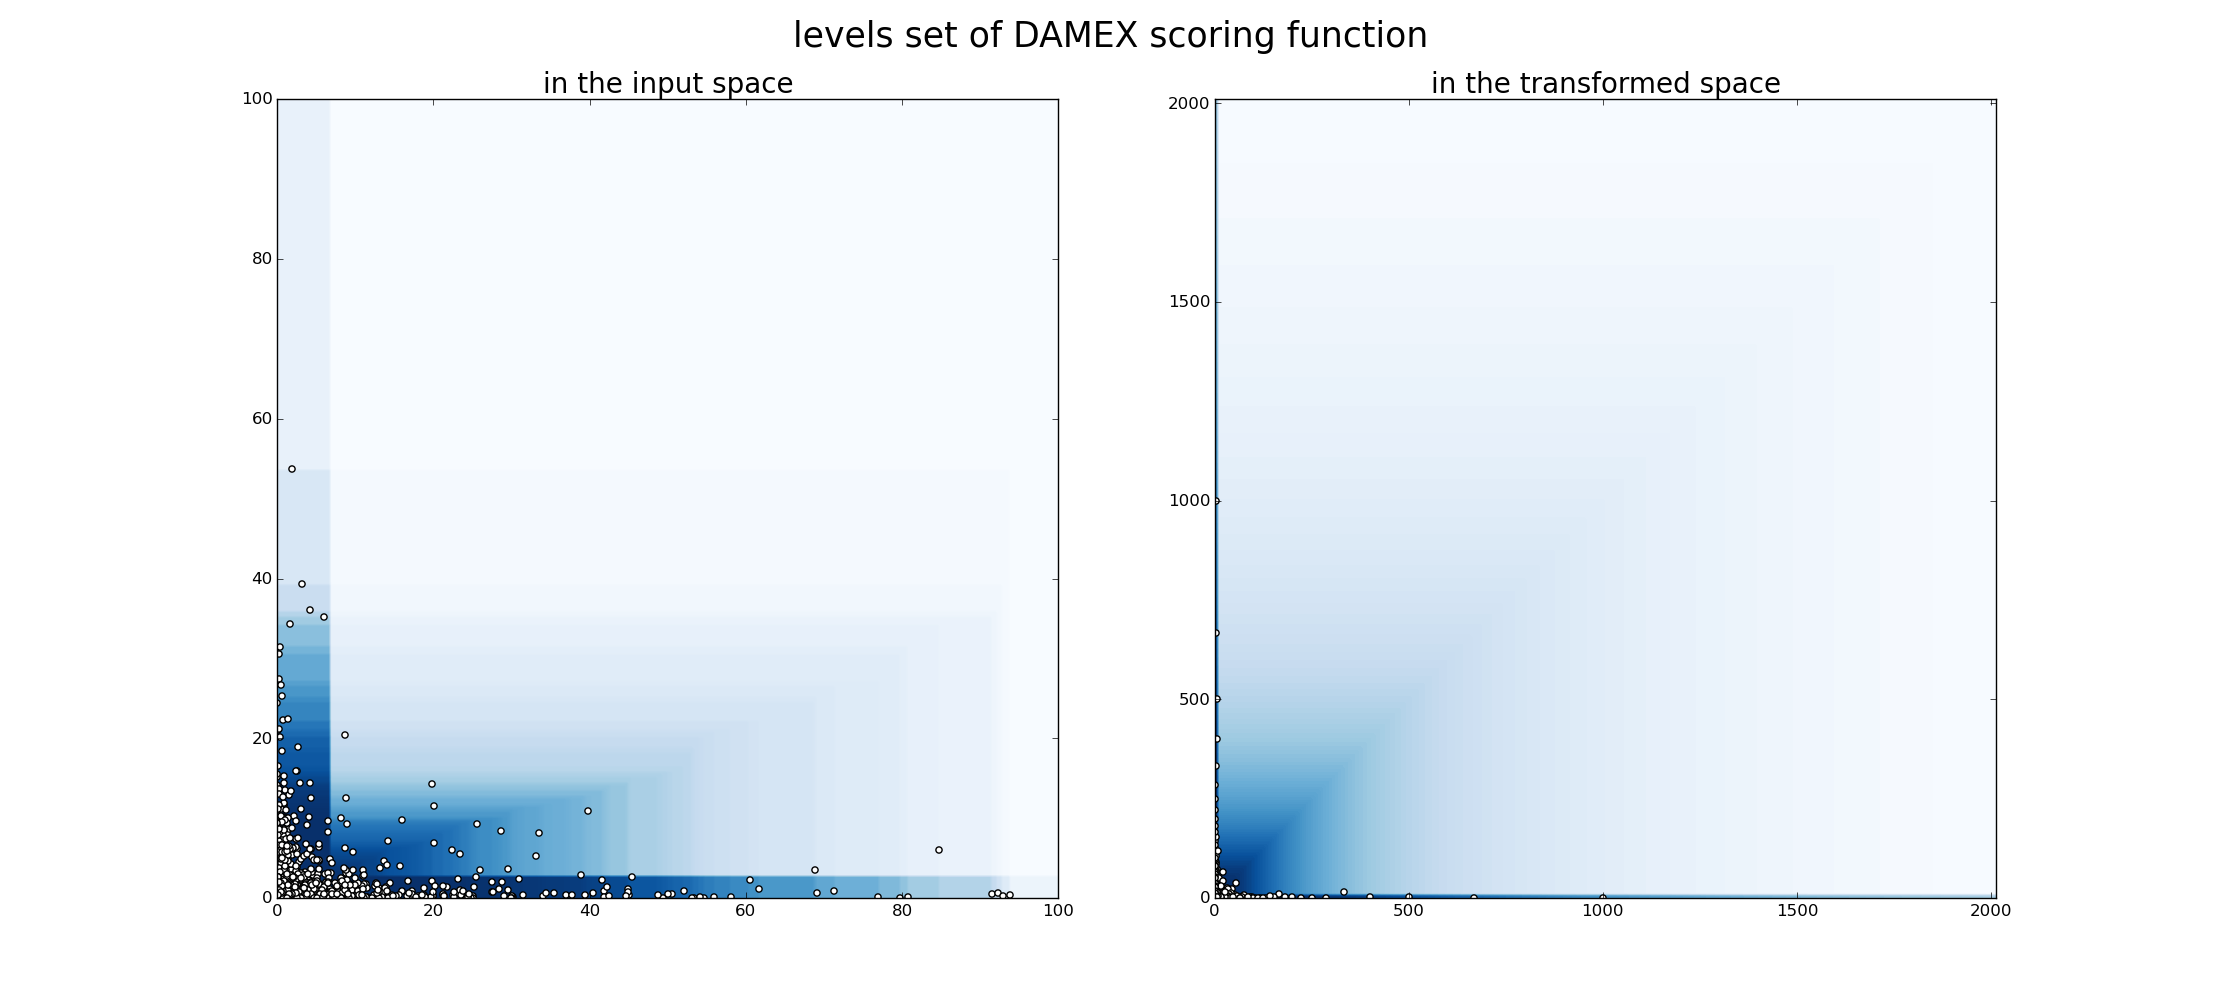
\includegraphics[scale=0.2331]{fig_source/plot_damex_level_sets.png}
\caption{Level sets of $s_n$ on simulated 2D data}
\label{jmva:DAMEX-2D}
\end{figure}

 This heuristic argument explains the following algorithm, referred to as {\it Detecting Anomaly with Multivariate EXtremes}  (DAMEX in abbreviated form). Note that this is a slightly modified version of the original DAMEX algorithm empirically tested in \cite{AISTAT16}, where $\epsilon$-thickened sub-cones instead of $\epsilon$-thickened rectangles are considered. The proof is more straightforward when considering rectangles and performance remains as good.
The complexity is in $O( dn\log n + dn) = O(dn\log n)$, where the first term on the left-hand-side comes from  computing the $\widehat F_j(X_i^j)$ (Step 1) by sorting  the data (\emph{e.g.} merge sort). The second one arises from Step 2. 

% \begin{center}
% \fbox{
% \begin{minipage}{0.95\linewidth}
\begin{algorithm}[!tbh]
\caption{DAMEX}
\label{jmva:DAMEX-algo}
{\bf Input:} parameters $\epsilon>0$,~~ $k = k(n)$,~~ $p\geq 0$.
\begin{enumerate}
\item Standardize \emph{via} marginal rank-transformation: $\mb{ \widehat V}_i:= \big (1/(1- \widehat F_j (X_i^j))\big)_{j=1,\ldots,d}$~.
\item Assign to each $\mb{\widehat V}_i$ the cone $R_\alpha^\epsilon$
  it belongs to.  
\item Compute $\hatmass(\alpha)$ from (\ref{jmva:heuristic_mu_n2})
   $\rightarrow$ yields: (small number of) cones with non-zero mass.
\item (Optional) Set to $0$ the $\hatmass(\alpha)$ below some small
  threshold defined in remark~\ref{jmva:rk:threshold} \wrt~$p$.%$\mu_{\min}\ge 0$ to eliminate cones with negligible mass
%\\$\rightarrow$ yields: (small number of) cones with non-zero mass
   $\rightarrow$ yields: (sparse) representation of the dependence
  structure 
 \begin{align}
 \label{jmva:phi_n}
\left\{\hatmass(\alpha):\; \emptyset\alpha\subset\{1,\ldots, d\}\right\}.%,~ \hatmass(\alpha)>\mu_{\min}\right\}.
% \Phi_n^\epsilon(v):= \sum_{\alpha} \hatmass(\alpha) \mathds{1}_{v \in \mathcal{C}_\alpha }
 \end{align}
\end{enumerate}
{\bf Output:} Compute the scoring function given
by~(\ref{jmva:def:scoring}), 
\begin{align*}
%\label{jmva:def:scoring}
s_n(\mb x):= (1/\|\widehat T(\mb x)\|_\infty)
\sum_{\alpha }%: \hatmass(\alpha)>\mu_{\min}} 
\hatmass(\alpha) \mathds{1}_{\widehat T(\mb x) \in R_\alpha^\epsilon}.
\end{align*}
\end{algorithm}
% \end{minipage}
% }
% \end{center}

Before investigating how the algorithm above empirically performs when applied to synthetic/real datasets, a few remarks are in order.


\begin{remark}({\sc Interpretation of the Parameters})
\label{jmva:rk_param_interpretation}
In view of %(\ref{jmva:eq:epsilonCone}) and
(\ref{jmva:heuristic_mu_n2}), $n/k$ is the threshold above  which the data are
considered as extreme and $k$ is proportional to the number of such
data, a common approach in multivariate extremes.  % A general
% heuristic in multivariate extreme is that $k$ is proportional to the
% number of data considered as extreme.
The tolerance parameter $\epsilon$ accounts for the  non-asymptotic nature of data. The
smaller $k$, the smaller $\epsilon$ shall be chosen. 
%{\red TODO : $\mu_{\min}$}
The additional angular mass threshold in step 4. acts as an additional
sparsity inducing parameter. Note that even without this additional
step (\ie\ setting $p=0$, the obtained representation for
real-world data (see Table~\ref{jmva:fig:wavedata-nb-faces})  is 
already sparse (the number of charges cones is significantly less than
$2^d$). % For the sake of simplicity, the present paper does not  investigate  the bias induced by $\mu_{\min}$ from a
% theoretical point of view (the main focus here 
% is on the role of $\epsilon$). However, experiments on AD datasets
% show an improved  performance when introducing this additional parameter.  
\end{remark}
\begin{remark}({\sc Choice of Parameters})
\label{jmva:rk_param_choice}
A standard choice of parameters $(\epsilon,~ k ,~ p)$ is
respectively 
$(0.01, n^{1/2}, 0.1)$. % where $\mu_{average}$ is the averaged mass of the non-empty sub-cones, \ie~$\mu_{average}=\mu_{total}/(\#$charged sub-cones)
However, there is no simple manner to choose optimally these parameters, as there is no simple way to determine how fast is the convergence to the (asymptotic) extreme behavior --namely how far in the tail appears the asymptotic dependence structure. Indeed, even though the  first term of the  error bound in Theorem~\ref{jmva:thm-princ} is  proportional, up to re-scaling, to $\sqrt{\frac{1}{\epsilon k} }+ \sqrt{\epsilon}$, which suggests choosing $\epsilon$ of order $ k^{-1/4}$, the unknown bias term perturbs the analysis and in practice, one obtains better results with the values above mentioned. 
In a supervised or novelty-detection framework (or if a small labeled dataset is available) these three parameters should be chosen by cross-validation.
In the unsupervised situation, a classical heuristic
(\cite{Coles2001}) is to choose $(k, \epsilon)$ in a stability region
of the algorithm's output: the largest $k$ (\emph{resp.} the larger
$\epsilon$) such that when decreased, the dependence structure remains
stable. This amounts to selecting as many  data as possible as being
extreme (\emph{resp. } in  low dimensional regions), within a stability
domain of the estimates, which exists under the primal assumption
\eqref{jmva:intro:assumption2} and in view of Lemma~\ref{jmva:lem:limit_muCalphaEps}. %constrained to observing the stability induced by the asymptotic behavior.
\end{remark}
\begin{remark} ({\sc Dimension Reduction})
If the extreme dependence structure is low dimensional, namely
concentrated on low dimensional cones $\mathcal{C}_\alpha$ -- or in other terms if only a
limited number of margins can be large together -- then most of the
$\widehat V_i$'s will be concentrated on the $R_\alpha^\epsilon$'s
such that  $|\alpha|$ (the dimension of the cone $\mathcal{C}_\alpha$)
is small; then the
representation of the dependence structure
% representation $\phi_n^\epsilon$
 in (\ref{jmva:phi_n}) is both sparse and low dimensional.
\end{remark}

\begin{remark} ({\sc Scaling Invariance})
DAMEX produces the same result if the input data are transformed in such a way that the marginal order is preserved. In particular, any marginally increasing transform or any scaling as a preprocessing step does not affect the algorithm. It also implies invariance with respect to any change in the measuring units. This invariance property constitutes part of the strength of the algorithm, since 
data preprocessing steps usually have a great impact on the overall performance and are of major concern in practice.
%looking for the best way to preprocess the data has a great influence on the performance and is a major concern in practice.
\end{remark}
% The next section provides a theoretical ground for Algorithm~\ref{jmva:DAMEX-algo}. 
% As shall be shown below, it  amounts to
% learning  the dependence structure of extremes (in particular, its support).
% The dependence parameter $\hatmass(\alpha)$ 
% % scoring function (\ref{jmva:def:scoring})
% actually coincides with a
% (voluntarily $\epsilon$-biased) natural estimator of $\mu(\mathcal{C}_\alpha)$, where $\mu$
% is  a `true' measure of the extremal dependence,
% namely the exponent measure defined as $\lim_{n \to \infty}
% \frac{n}{k} \mathbb{P} \left[V \in \frac{n}{k}~ (\point) \right] $.
% Section~\ref{jmva:sec:estimation} develops uniform, non-asymptotic upper
% bounds on  the error 
% $|\hatmass(\alpha) - \mu(\mathcal{C}_\alpha)|$ to attest the theoretical quality of this estimate.
% Providing empirical result on simulated and real data.
% The two following sections are to prove an inequality (Theorem \ref{jmva:thm-princ}) of type 
% \begin{align*}
% |\mu_n(\mathcal{C}_\alpha^\epsilon) - \mu(\mathcal{C}_\alpha)| ~\le~ \left( \frac{C \sqrt d}{k^{1/4}} \sqrt{ \log\frac{d}{\delta}} ~+~ b(n) \right)
% \end{align*}
% with $b(n)$ the model biais, $\mu_n(\mathcal{C}_\alpha^\epsilon) = \hatmass(\alpha)$, and $\mu$ the `true measure of the extreme behavior' namely the exponent measure defined as $\lim_{n \to \infty} \frac{n}{k} \mathbb{P} \left[V_1 \in \frac{n}{k}~. \right] $ in the sense of the weak convergence, where $V_i:= \left ( \frac{1}{1- F_j (X_i^l)}\right)_{l=1..d}$.

%%% Local Variables: 
%%% mode: latex
%%% TeX-master: t
%%% End: 

\section{Experimental results}
\label{jmva:sec:experiments}
%\subsection{Sparse dependence structure of real data}
\subsection{Recovering the support of the dependence structure of generated data}
Datasets of size $50000$ (respectively $100000$, $150000$) are  generated in $\mathbb{R}^{10}$ according to a popular multivariate extreme value
model, introduced by \cite{Tawn90},  namely a multivariate asymmetric
logistic distribution ($G_{log}$). %  one
% model ,
The data have the following features: (i) they resemble `real life'
data, that is, the $X_i^j$'s are non
zero  and the transformed $\hat V_i$'s belong to the interior cone
$\mathcal{C}_{\{1,\ldots,d\}}$, (ii) the associated (asymptotic) exponent measure concentrates on
 $K$ disjoint cones $\{\mathcal{C}_{\alpha_m} , 1\le m\le K\}$.  % where the
 % $D = \{\alpha_m , 1\le m\le k\}$ is a partition of $\{1,\ldots d\}$  (the latter requirement simplifies the
 % model's specification). Note that, in this context, the number of
 % `non-zero' faces is $K\le d$.
 For the sake of reproducibility, % we give the
 % expression for the \emph{c.d.f.} $G$ from which the data is
 % drawn,  % Here, $D = \{\alpha_1,\ldots\alpha_k\}$ denote the disjoint
 % % subsets of indices such that $\mu(\mathcal{C}_{\alpha_m})\neq 0$,
 % % $m\le k$.
 $$ G_{log}(\mb x) = \exp\{ - \sum_{m = 1}^K \left(\sum_{j \in \alpha_m}
     (|A(j)|x_j)^{ - 1/{w_{\alpha_m}}}\right)^{w_{\alpha_m}} \}, $$
 where $|A(j)|$ is the cardinal of the set $\{\alpha\in D: j \in
 \alpha\}$ and where $w_{\alpha_m} = 0.1$ is a dependence parameter
 (strong dependence). %  in
 % $(0,1]$ that we set to $0.1$ : the dependence on
 % $\mathcal{C}_{\alpha_m}$ is a decreasing function of
 % $w_{\alpha_m}$.
 % For our simulations, $w_{\alpha_m}$ is set to $0.1$.
% We simulate 50000 observations of a multivariate asymmetric logistic
% model in $\mathbb{R}^{10}$, introduced by \cite{Tawn90}. 
%  and whose exponent measure is $\mu([0, \mb x]^c) = -\log(G_0(\mb x))$ with 
% \begin{align*}
% G_0(x) = \sum_{\alpha \in A} \left(\sum_{i \in \alpha} \left(\frac{\theta_{i,\alpha}}{x_i} \right)^{1/w_\alpha}\right)^{w_\alpha} .
% \end{align*}
% Here $A$ is the set of all non-empty subsets of $\dd$,
% $\theta_{i,\alpha} = 0$ for all $\alpha \notin D$, $D \dd \setminus \emptyset $ is a subset of faces,
% and $\theta_{i,\alpha} = \frac{1}{|A_{(i)}|}$ with $|A_{(i)}|$ is the cardinal of the set $A_{(i)} = \{\alpha \in A, i \in \alpha\}$. Note that for each subset of features $\alpha$, either the $\theta_{i,\alpha}$ are all null, either they are all positive. We choose $w_\alpha$ to be $1$ for every $\alpha$, since we want a maximal asymptotic dependence between the chosen subsets of features (namely the $\alpha$ such that $\forall i,~\theta_{i,\alpha} \neq 0$). This simulation thus consider only two cases for each subset of features $\alpha$: either they are dependent and there is a non-negligeable asymptotic mass on the corresponding face (charged by $\mu$); either they are independent and have thus no mass asymptotically ($\mu$ has no mass on such faces).
The data are simulated using  Algorithm 2.2 in \cite{Stephenson2003}.
The subset of sub-cones $D$ charged by $\mu$ is randomly chosen (for each
fixed number of sub-cones $K$) and the purpose is to recover $D$ by Algorithm~\ref{jmva:DAMEX-algo}.
  For each $K$, $100$ experiments
are made and we consider  the  number of `errors', that is,      the number of
non-recovered or false-discovered sub-cones. Table~\ref{jmva:table:logevd} shows the averaged
numbers of errors  among the $100$ experiments. %% (multiplied by $100$ for
%%readability). 
\begin{table}[!ht]
\caption{Support recovering on simulated data}
\label{jmva:table:logevd}
\centering
\resizebox{\linewidth}{!} {
\begin{tabular}{c ccccccccccc}
  \toprule
  $\#$ sub-cones $K$       &    3 & 5    &  10   & 15   & 20    & 25  & 30   & 35    & 40    & 45    & 50 \\
  \midrule
 Aver. $\#$ errors ~~(n=5e4)     & 0.02 & 0.65 & 0.95  & 0.45 & 0.49  & 1.35& 4.19 & 8.9  & 15.46  & 19.92  & 18.99 \\
   %(n=5e4)     &&&&&&&&&&& \\

 Aver. $\#$ errors (n=10e4)    & 0.00 & 0.45 & 0.36  & 0.21 & 0.13  & 0.43& 0.38 & 0.55  & 1.91  & 1.67  & 2.37 \\
%   (n=10e4)     &&&&&&&&&&& \\

 
 Aver. $\#$ errors (n=15e4)    & 0.00  & 0.34 & 0.47 & 0.00 & 0.02  & 0.13& 0.13 & 0.31  & 0.39  & 0.59  & 1.77 \\
%(n=15e4) &&&&&&&&&&& \\
 % Aver. $\#$ errors (n=15e4)    & 0.01 & 0.01 & 0.06  & 0.02 & 0.39  & 1.12& 1.82 & 3.59  & 6.59  & 8.06  & 11.21 \\fi
 %  \hline
  \bottomrule
\end{tabular}
}
\end{table}
The results are very promising in situations where the number of sub-cones is moderate \emph{w.r.t.} the number of observations. %  Also, additional experiments (not shown here) indicate

\subsection{Sparse structure of extremes  (wave data)}
Our goal is here to verify that the two expected phenomena mentioned
in the introduction, \textbf{1-}~sparse dependence structure of extremes (small number
of sub-cones with non zero mass), \textbf{2-}~low dimension of the
sub-cones with non-zero mass,  do occur with real data. 
%We test the sparsity in the extreme dependence structure of 
We consider wave
directions data provided by Shell, which consist of $58585$
measurements  $D_i$, $i\le 58595$ of wave directions between $0^{\circ}$ and $360^{\circ}$ at $50$ different
locations (buoys in North sea). The dimension is thus $50$. % , each sample
% representing a different record time.
The angle $90^{\circ}$ being fairly
rare, we work with data obtained as $X_i^j = 1/(10^{-10} + |90-
D_i^j|)$, where $D_i^j$ is the wave direction at buoy $j$, time $i$. Thus,
$D_i^j$'s close to $90$ correspond to  extreme $X_i^j$'s.
% we chose to apply the transform $1/(1e^{-10} + \|90-.\|)$ to the
% data in order to make it
% extreme. % extremes the $90$ degree observations
Results in
% Figure~\ref{jmva:fig:wavedata-dim}~and
Table~\ref{jmva:fig:wavedata-nb-faces}% ($\mu_{total}$ denotes the total probability mass of $\mu$)
show that 
the %dimensions 
number of  sub-cones $\mathcal{C}_\alpha$ identified by Algorithm~\ref{jmva:DAMEX-algo}
is indeed small compared to the total number of sub-cones ($2^{50}$-1).
% supporting the  extreme data  
%%are  essentially lower than $15$
(Phenomenon \textbf{1} in the introduction section). 
Further, the dimension of these sub-cones is essentially moderate
(Phenomenon \textbf{2}):
respectively $93\%$, $98.6\%$ and  $99.6\%$
of the mass is affected to  sub-cones of dimension no greater  than $10$,
$15$ and $20$ respectively %  ???????????,
% with a maximal dimension of ?????????? 
(to be compared with $d=50$).  Histograms displaying the mass repartition produced by Algorithm~\ref{jmva:DAMEX-algo} are given in Fig.~\ref{jmva:fig:wavedata-dim}.
% and
% their  number is %of such faces charged by the exponent measure $\mu$ is
% small (phenomenon \textbf{1}) compared to the total number of sub-cones ($2^{50}$-1).
\begin{figure}[!ht]
\centering
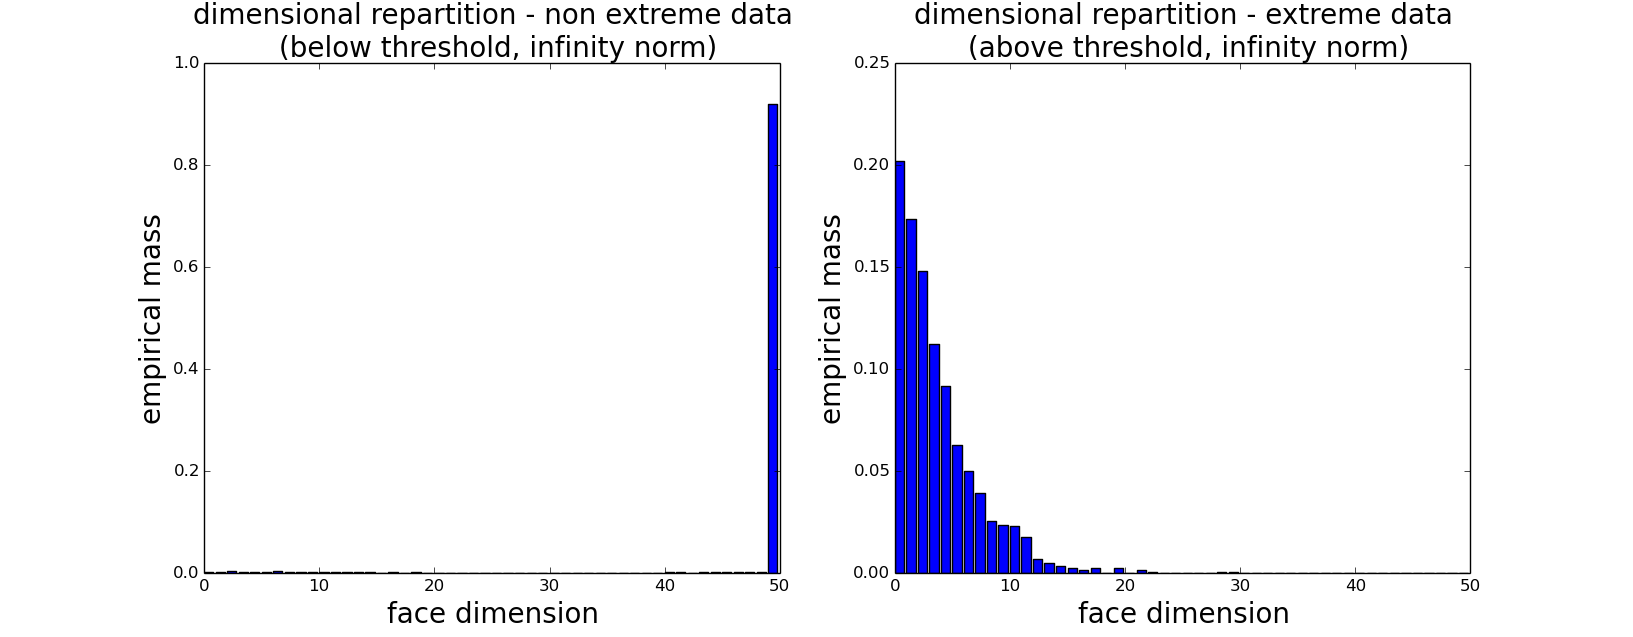
\includegraphics[scale=0.33]{fig_source/wave_dir2}
\caption{sub-cone dimensions of wave data}
\label{jmva:fig:wavedata-dim}
\end{figure}

\begin{table}[!ht]
\caption{Total number of sub-cones of wave data}
\label{jmva:fig:wavedata-nb-faces}
\centering
%\resizebox{\linewidth}{!} {
\begin{tabular}{lcc}
\toprule
~ & non-extreme data & extreme data \\
\midrule
nb of sub-cones with mass $>0$ ($p = 0$) & 3413 & 858 \\
idem after thresholding ($p = 0.1$) & 2 & 64 \\
idem after thresholding ($p = 0.2$) & 1 & 18 \\ 
\bottomrule
\end{tabular}
%}
\end{table}


\subsection{Application to Anomaly Detection on real-world data sets}

% \noindent
% \begin{minipage}{0.5\linewidth}
% \centering
% \includegraphics[scale=0.17]{fig_source/extreme_AD}
% \captionof{figure}{\tiny Combination of any standard AD algorithm with DBAD}
% \label{jmva:fig:combination}
% \end{minipage}\hfill
% \begin{minipage}{0.5\linewidth}
% \end{minipage}
%We point out that
 The main purpose of Algorithm~\ref{jmva:DAMEX-algo} is to build a 
 `normal profile' for 
extreme data, so as to distinguish between normal and ab-normal
extremes. 
In this section we evaluate its performance %on such region
 and compare it with that of a standard anomaly detection algorithm, %  that it may be combined with a
% standard AD algorithm  to handle extreme \emph{and} non-extreme data,
% improving the global performance of the chosen standard algorithm.
% In this section we show that it may be combined with a
% standard AD algorithm  to handle extreme \emph{and} non-extreme data,
% improving the global performance of the chosen standard algorithm.
% which focusing on non-extreme data. 
% This can be done as
% illustrated in Fig.~\ref{jmva:fig:combination} by splitting the input
% space between an extreme region and a non-extreme one, then applying
% Algorithm~\ref{jmva:DAMEX-algo} to the extreme region, while the
% non-extreme one is processed with the standard
% algorithm.
the Isolation Forest (iForest)
algorithm, which we chose in view of its
established high performance (\cite{Liu2008}). 
The two algorithms are trained and tested on the same datasets, the
test set being restricted to an  extreme region.
% Our aim is to compare the results obtained with the
% combined method
%  `iForest + DAMEX' above described, to those obtained with iForest
%  alone on the whole input space. 
% A random forest AD algorithm is chosen as an exemplary `standard' one,
% namely the Isolation Forest (iForest) algorithm (in view of its high performances)
% . We compare its own use, with when combined with Algorithm~\ref{jmva:DAMEX-algo} as illustrated in Figure~\ref{jmva:fig:combination}.
 Five reference anomaly detection datasets  are considered:
 \emph{shuttle}, \emph{forestcover}, \emph{http},
 \emph{SF} and \emph{SA} \footnote{These datasets are available for instance on http://scikit-learn.org/dev/ }. The experiments are performed in a
 novelty detection framework (the training set consists of normal data). 
% In a  non-supervised framework (training set including abnormal data), the
%  improvements brought by the use of DAMEX are less significant, but the
%  precision score is still increased % on five datasets out of six, 
%  when the recall is high (high rate of true positives), inducing more vertical ROC curves near the origin.
%
 % When done on both normal and abnormal data, the results are less impressive but there is still an improvement of the precision on five of the six datasets when the recall is high (namely when the true positive rate is large).
%

The \emph{shuttle} dataset is the fusion of the training and testing datasets
available in the UCI repository \cite{Lichman2013}. The data have $9$
 numerical attributes,  the first one being time. Labels from $7$ different classes are also
 available. Class $1$ instances are considered as normal, the others as anomalies. 
We use instances from all different classes but class $4$,  % classes $1, 2,3,5,6$ and $7$ (class In our experiments, the class $1$ is considered as normal and instances from class $2, 3, 5, 6, 7$ are anomalies,
which yields an anomaly ratio (class 1) of $7.17\%$. %
%Instances from class $4$ are not used.
%

In the \emph{forestcover} data, also available at UCI
repository (\cite{Lichman2013}), the normal data are the  instances
from class~$2$ while instances from class $4$ are anomalies, other classes are omitted, 
so that the  anomaly ratio for this dataset is  $0.9\%$. 
%

The last three datasets belong to the KDD Cup '99 dataset
(\cite{KDD99}, \cite{Tavallaee2009}), produced by processing the
tcpdump portions of the 1998 DARPA Intrusion Detection System (IDS)
Evaluation dataset, created by MIT Lincoln Lab \cite{Lippmann2000}.
The artificial data was generated using a closed network and a wide
variety of hand-injected attacks (anomalies) to produce a large number
of different types of attack with normal activity in the background.
Since the original demonstrative purpose of the dataset concerns
supervised anomaly detection, the anomaly rate is very high ($80\%$), which is
unrealistic in practice, and inappropriate for evaluating the
performance on realistic data.  We thus take standard pre-processing
steps in order to work with smaller anomaly rates. For datasets
\emph{SF} and \emph{http} we proceed as described in
\cite{Yamanishi2000}: \emph{SF} is obtained by picking up the data
with positive logged-in attribute,
and %using only four attributes thus
focusing on the intrusion attack, which gives an anomaly proportion of
$0.48\%.$ %$0.3\%$.
The dataset \emph{http} is a subset of \emph{SF} corresponding to a
third feature equal to 'http'.
%
Finally, the \emph{SA} dataset  is obtained as in \cite{Eskin2002} by 
selecting all the normal data, together with a small proportion
($1\%$) of anomalies. % abnormal data  % to gives an anomaly proportion of $1\%$.
% Moreover, the 3 categorical
% attributes have been binary encoded.
%

Table~\ref{jmva:table:data} summarizes the characteristics of these
datasets. 
The thresholding parameter $p$ is fixed to $0.1$, the averaged mass of the non-empty sub-cones, while the parameters $(k,\epsilon)$ are standardly chosen as $(n^{1/2}, 0.01)$.
The extreme region on which the evaluation step is performed is chosen
as $\{\mb x:~ \|T(\mb x)\| > \sqrt{n} \}$, where $n$ is the  training
set's sample size. The ROC and PR curves are computed using only observations in the extreme region. This provides a precise evaluation of the two anomaly detection methods on extreme data.
 % As the datasets \emph{http}, \emph{smtp} and \emph{SF} do not have enough features to consider the stability, we choose the (standard) parameters $(k, \epsilon) = (n^{1/2}, 0.01)$. 
For each of them, 20 experiments on random training and testing datasets are performed, yielding averaged ROC and Precision-Recall curves whose AUC are presented in Table~\ref{jmva:table:results-dbad+iforest-01}.
%
DAMEX significantly improves the performance (both in term of precision and of ROC curves) in extreme regions
for each dataset, as illustrated in figures \ref{jmva:fig:shuttle} and \ref{jmva:fig:SF}.

In Table~\ref{jmva:table:results-dbad+iforest-1}, we repeat the same experiments but with $\epsilon=0.1$.
This yields the same strong performance of DAMEX, excepting for \emph{SF} (see Figure~\ref{jmva:fig:SF_1}).
Generally, to large $\epsilon$ may yield over-estimated
$\hatmass(\alpha)$ for low-dimensional faces $\alpha$.
Such a performance gap between $\epsilon=0.01$ and $\epsilon=0.1$ can also be explained by the fact that anomalies may form a cluster which is wrongly include in some over-estimated `normal' sub-cone, when $\epsilon$ is too large. Such singular anomaly structure would also explain the counter performance of iForest on this dataset.

% on this dataset with $\epsilon=0.1$, DAMEX has lower performance than iForest. Its ROC
% curve has a slow slope at the origin (Fig.~\ref{jmva:fig:SF}), which reflects a lack of
% precision when assigning high abnormal scores. This may be explained
% by the fact that % anomalies belong to some low dimensional faces for which
% the estimate
% $\hatmass(\alpha)$ is too biased (over-estimated) for low-dimensional faces $\alpha$, using a too large tolerance parameter $\epsilon$, and can even wrongly include anomalies which were in the central cone, despite quite close to the border.

% , or by the simple fact that the asymptotic dependence
% structure has not quite been reached at this level $k = n^{1/2}$.
%on this dataset, the algorithm seems unable to capture any extreme
%dependence structure, either because the latter is non-existent (no
%regularly varying tail), either because the convergence is too slow
%to appear in our relatively small dataset.
%
% Smaller values of $\epsilon$ reduce the bias and Fig.~\ref{jmva:fig:SF-01}
% shows that decreasing $\epsilon$ clearly improves the performance
% on regions where the abnormality score is large (near the origin on
% the ROC and Precision/Recall plots). 

We also point out that for very small values of epsilon ($\epsilon \le 0.001$),
the performance of DAMEX significantly decreases on these datasets.
With such a small $\epsilon$, most observations belong to the central cone
(the one of dimension $d$) which is widely over-estimated, while the other cones are under-estimated.%  and no discrimination measure
% appears except the norm of the observations.

The only case were using very small $\epsilon$ should be useful, is when the asymptotic behaviour is
clearly reached at level $k$ (usually for very large threshold $n/k$, \eg~$k=n^{1/3}$), or in the
specific case where anomalies clearly concentrate in low dimensional sub-cones: The use of a small $\epsilon$ precisely allows
to assign a high abnormality score to these sub-cones (under-estimation of the asymptotic mass), which yields better performances.

% While Fig.~\ref{jmva:fig:SF} displays the ROC and
% PR curves for the standard parameter $\epsilon = 0.1$,
% Fig.~\ref{jmva:fig:SF-01} shows the same
% curves obtained with $\epsilon=0.01$. For
% this dataset, decreasing $\epsilon$ clearly improves the performance
% on regions where the abnormality score is large (near the origin on
% the ROC and Precision/Recall plots). 

% With
% such a small $\epsilon$, more observations belong to the central cone
% (the one of dimension $d$). It is then difficult to detect anomalies
% in this cone if their radius are not larger than the normal
% observations. However, if the anomalies are concentrated in smaller
% dimensional subcones, those subcones are possibly over-estimated using
% too large $\epsilon$. The use of a smaller $\epsilon$ precisely allows
% to assign a high abnormality score to these subcones, which yields
% better performances.
The averaged ROC curves and PR curves for the other datasets are represented in Figures
\begin{table}[!ht]
\caption{Datasets characteristics}
\label{jmva:table:data}
\centering
%\footnotesize
\begin{tabular}{lccccc}
  \toprule
   ~                   & shuttle & forestcover & SA     & SF     & http    \\
  \midrule
  Samples total        & 85849   & 286048      & 976158 & 699691 & 619052  \\
  Number of features   & 9       & 54          & 41     & 4      & 3       \\
  Percentage of anomalies & 7.17    & 0.96        & 0.35   & 0.48   & 0.39 \\
\bottomrule
\end{tabular}
\end{table}

%TODO: rappel PR et ROC
\begin{table}[!ht]
\caption{Results on extreme regions with standard parameters $(k,\epsilon) = (n^{1/2}, 0.01)$}
\label{jmva:table:results-dbad+iforest-01}
\centering
\begin{tabular}{lcccc}
  \toprule
Dataset      &\multicolumn{2}{c}{iForest}& \multicolumn{2}{c}{DAMEX}\\\hline
~            &AUC ROC       & AUC PR     &AUC ROC     &AUC PR       \\
shuttle      & 0.957        & 0.987      &$\mb{0.988}$&$\mb{0.996}$ \\
forestcover  & 0.667        & 0.201      &$\mb{0.976}$&$\mb{0.805}$ \\
http         & 0.561        & 0.321      &$\mb{0.981}$&$\mb{0.742}$ \\
%smtp         & $\mb{0.900}$ &$\mb{0.004}$&0.898       &0.003        \\
SF           & 0.134        & 0.189      &$\mb{0.988}$&$\mb{0.973}$ \\
SA           & 0.932        &0.625       &$\mb{0.945}$&$\mb{0.818}$ \\ 
\bottomrule
\end{tabular}
\end{table}


\begin{table}[!ht]
\caption{Results on extreme regions with lower $\epsilon=0.1$}
\label{jmva:table:results-dbad+iforest-1}
\centering
\begin{tabular}{lcccc}
  \toprule
Dataset      &\multicolumn{2}{c}{iForest}& \multicolumn{2}{c}{DAMEX}\\\hline
~            &AUC ROC       & AUC PR     &AUC ROC     &AUC PR       \\
shuttle      & 0.957        & 0.987      &$\mb{0.980}$&$\mb{0.995}$ \\
forestcover  & 0.667        & 0.201      &$\mb{0.984}$&$\mb{0.852}$ \\
http         & 0.561        & 0.321      &$\mb{0.971}$&$\mb{0.639}$ \\
%smtp         & $\mb{0.900}$ &$\mb{0.004}$&0.898       &0.003        \\
SF           & $\mb{0.134}$ & 0.189      &0.101       &$\mb{0.211}$ \\
SA           & 0.932        &0.625       &$\mb{0.964}$&$\mb{0.848}$ \\ 
\bottomrule
\end{tabular}
\end{table}


\begin{figure}[!ht]
  \centering
  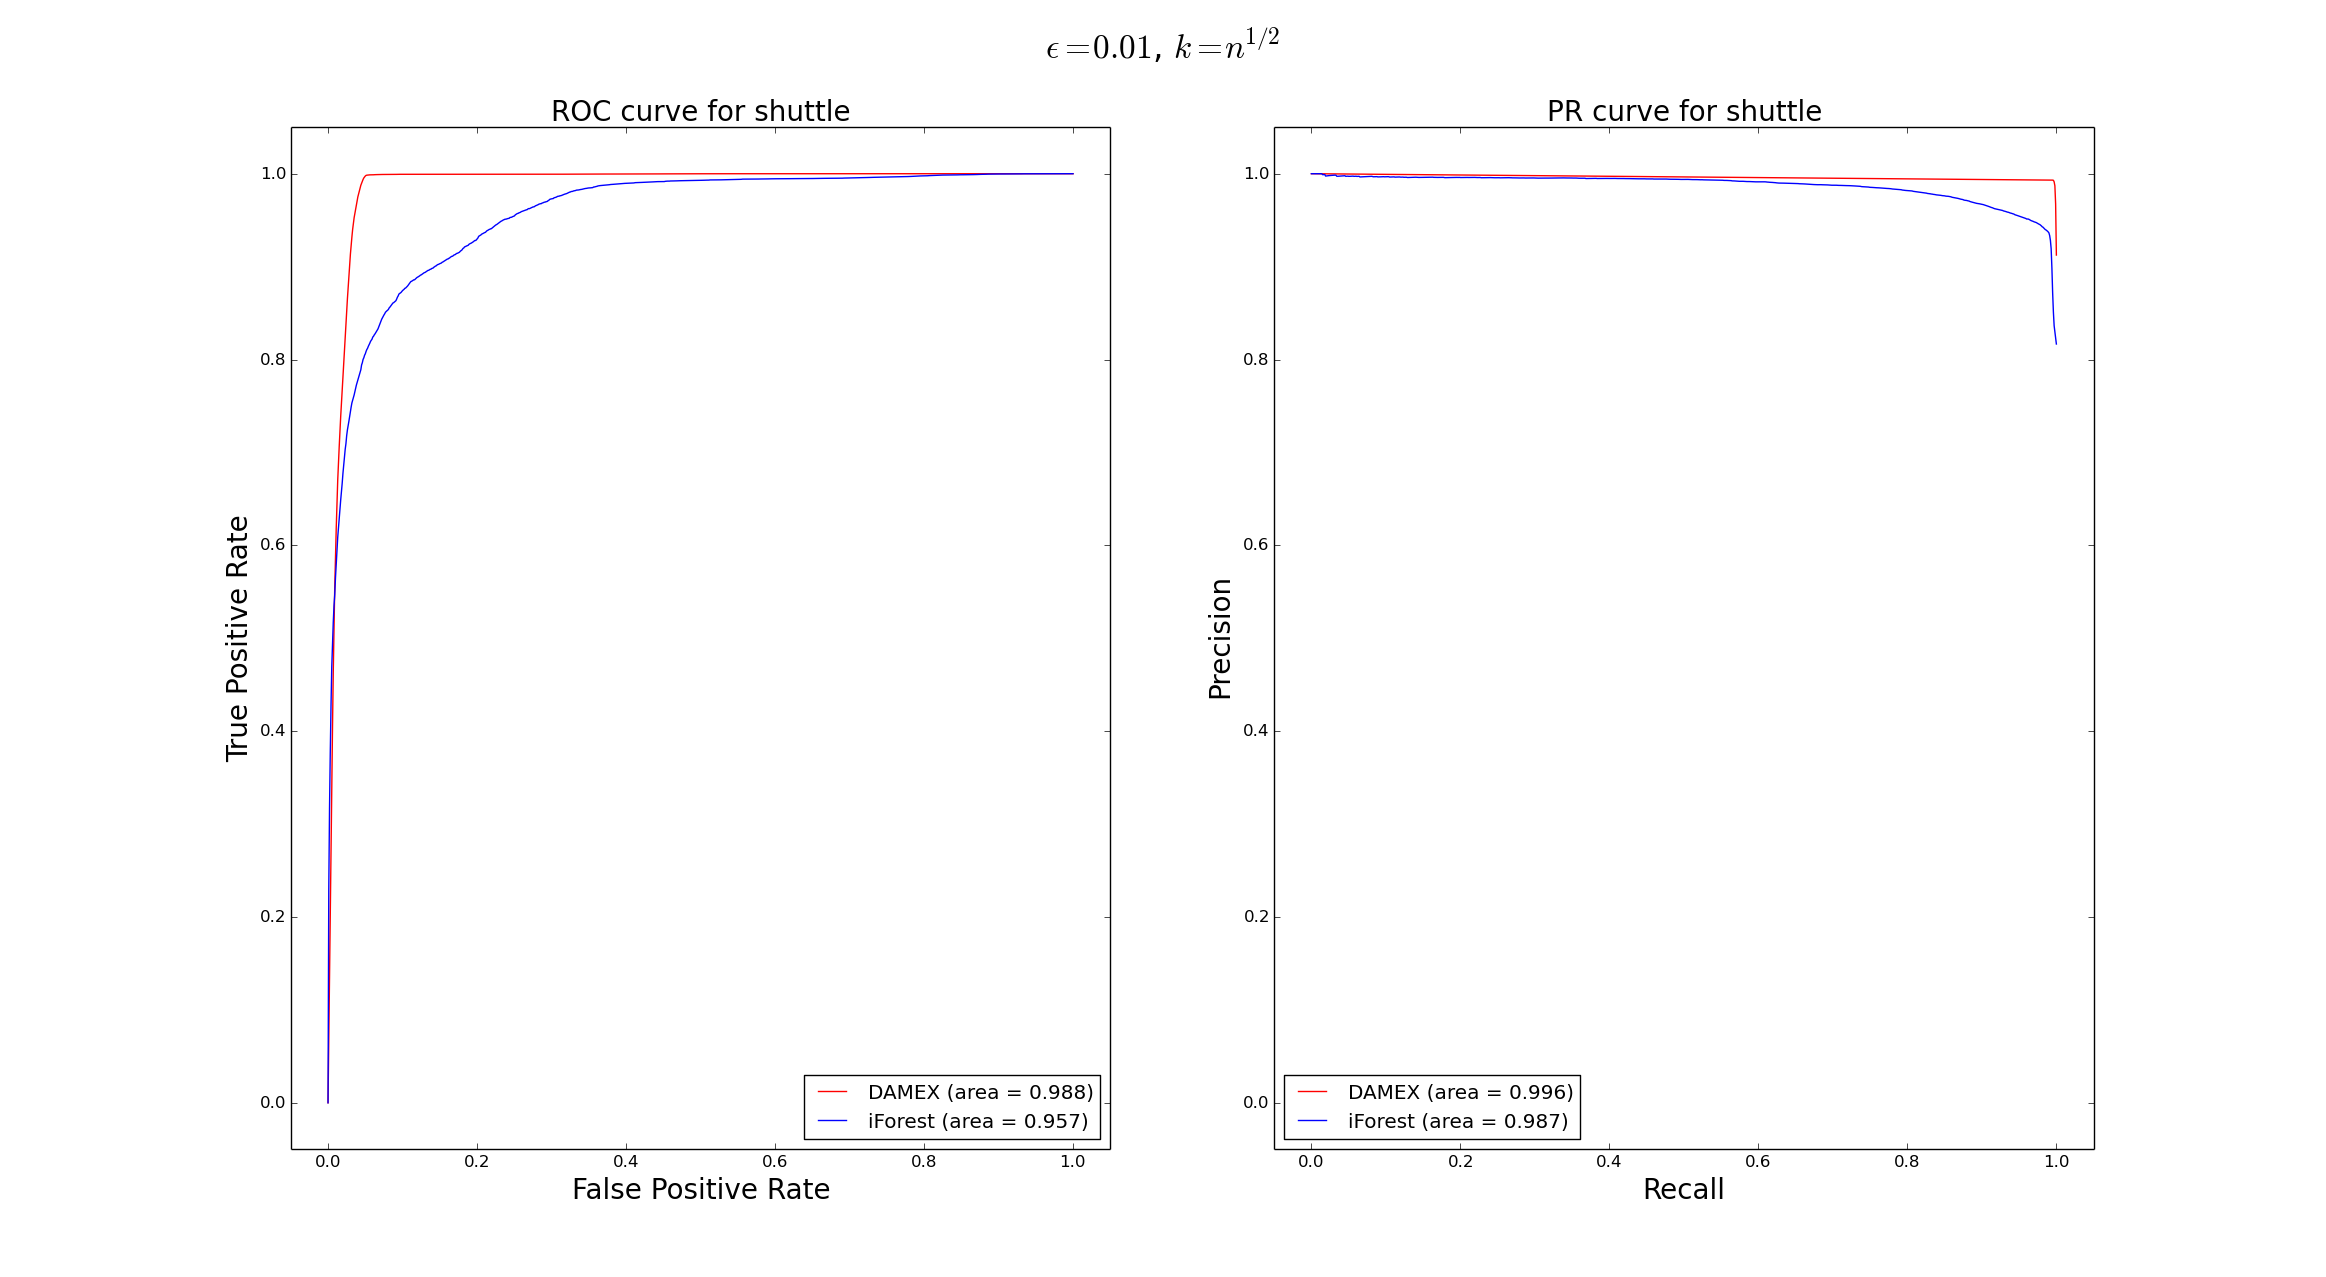
\includegraphics[width = \textwidth]{fig_source/shuttle-semi-supervised-average-rect-01.png}
  \caption{SF dataset, default parameters}
\label{jmva:fig:shuttle}
\end{figure}
\begin{figure}[!ht]
  \centering
  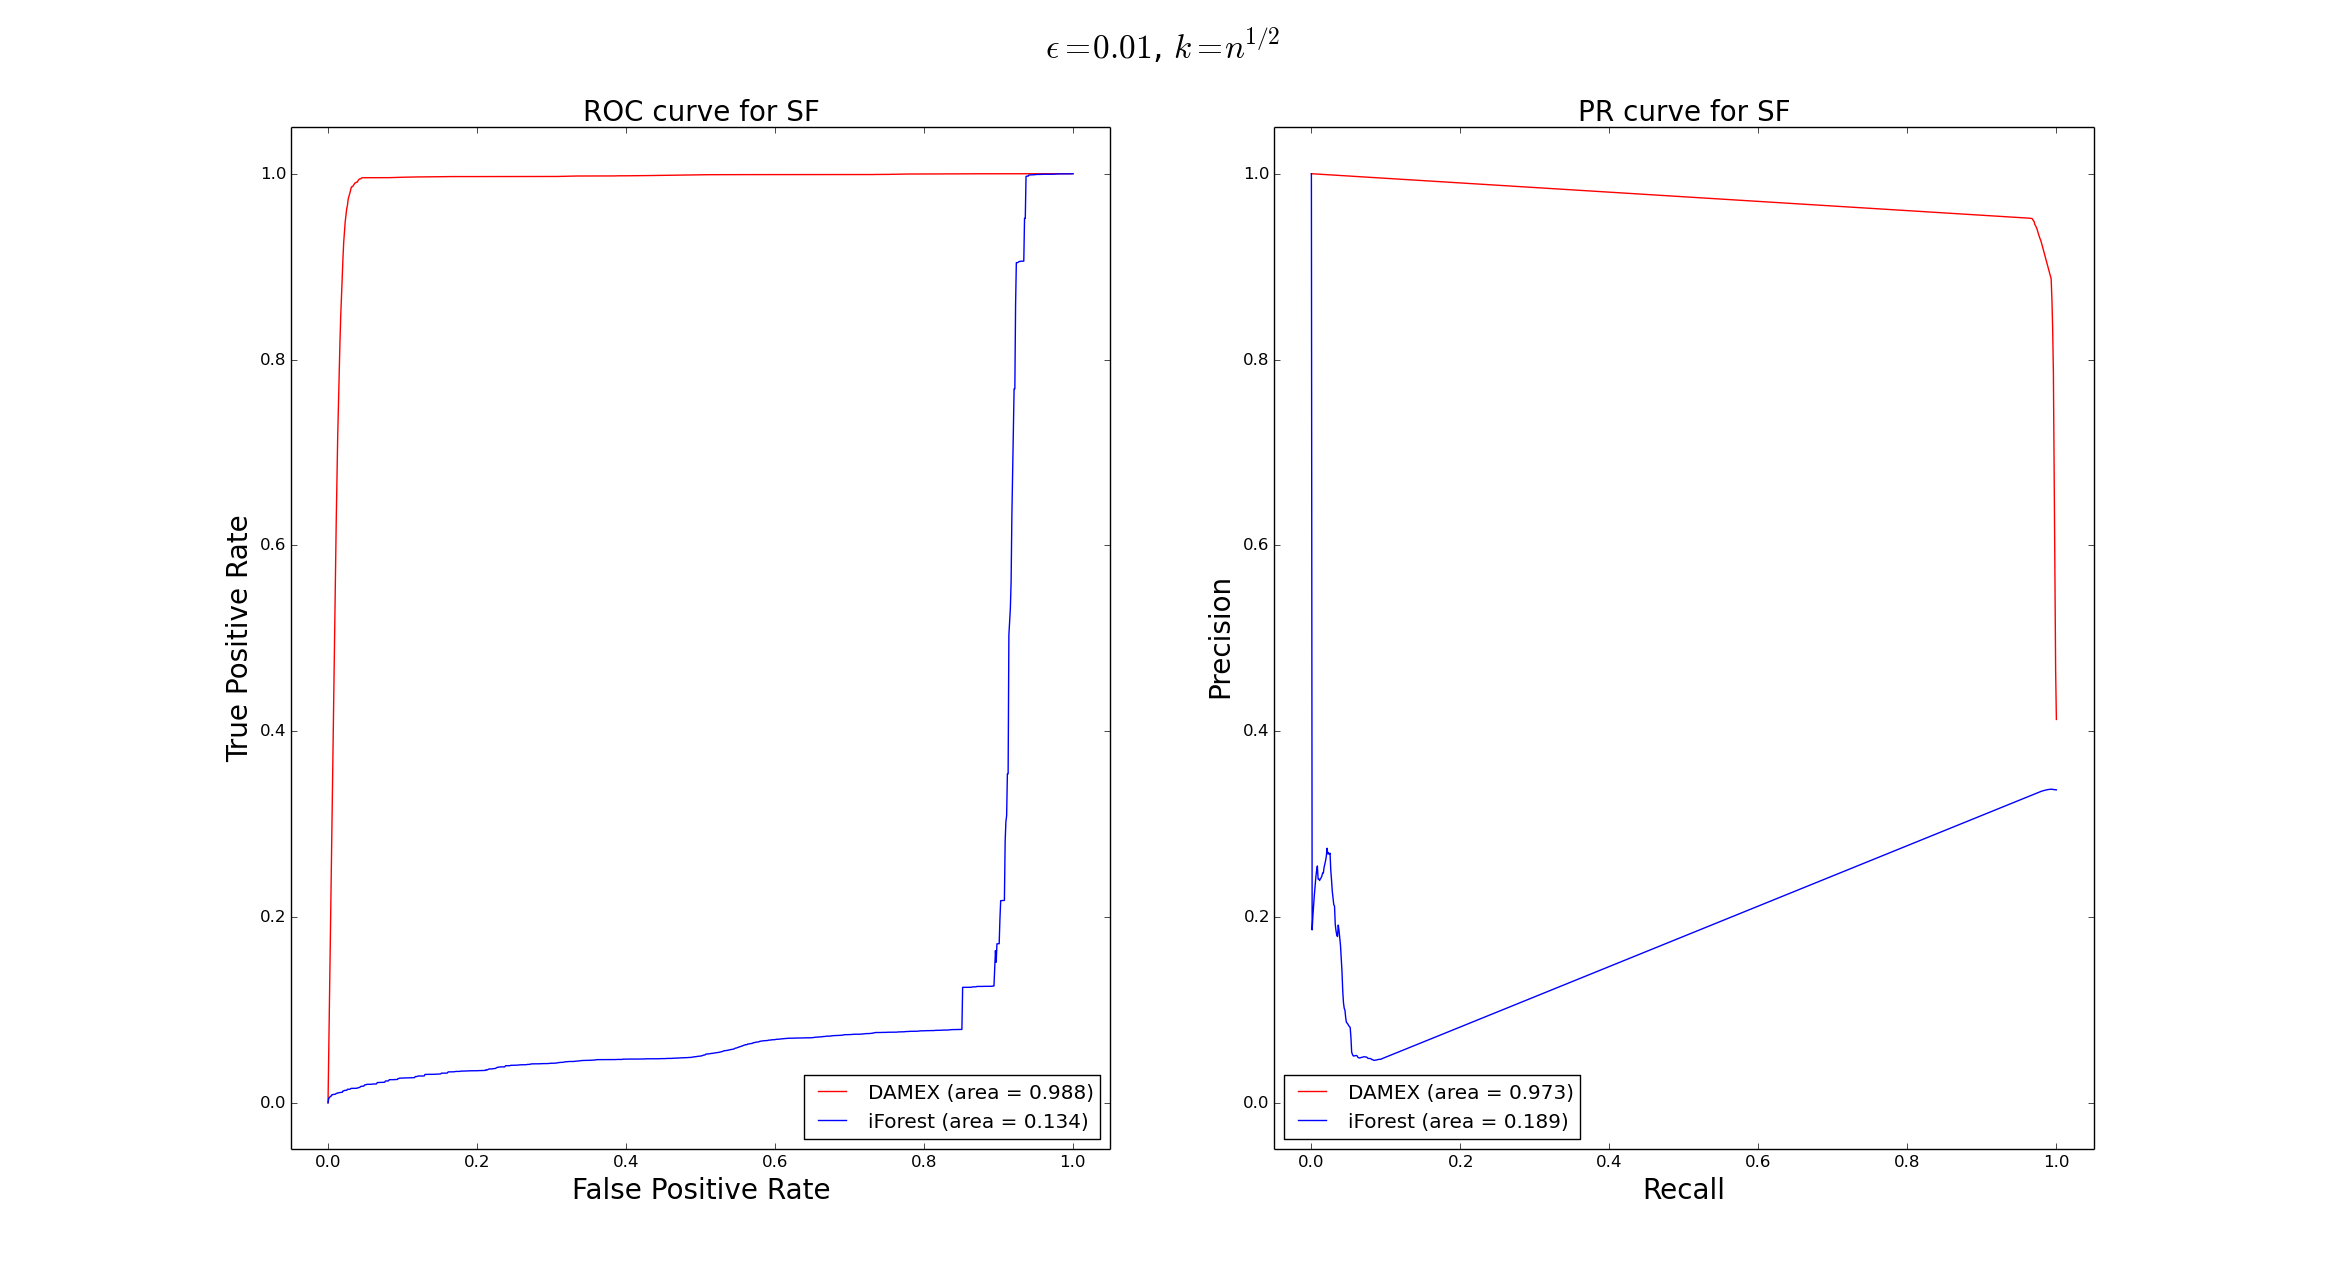
\includegraphics[width = \textwidth]{fig_source/SF-4d-lb-semi-supervised-average-rect-01}
  \caption{SF dataset, larger $\epsilon$}
\label{jmva:fig:SF}
\end{figure}
\begin{figure}[!ht]
  \centering
  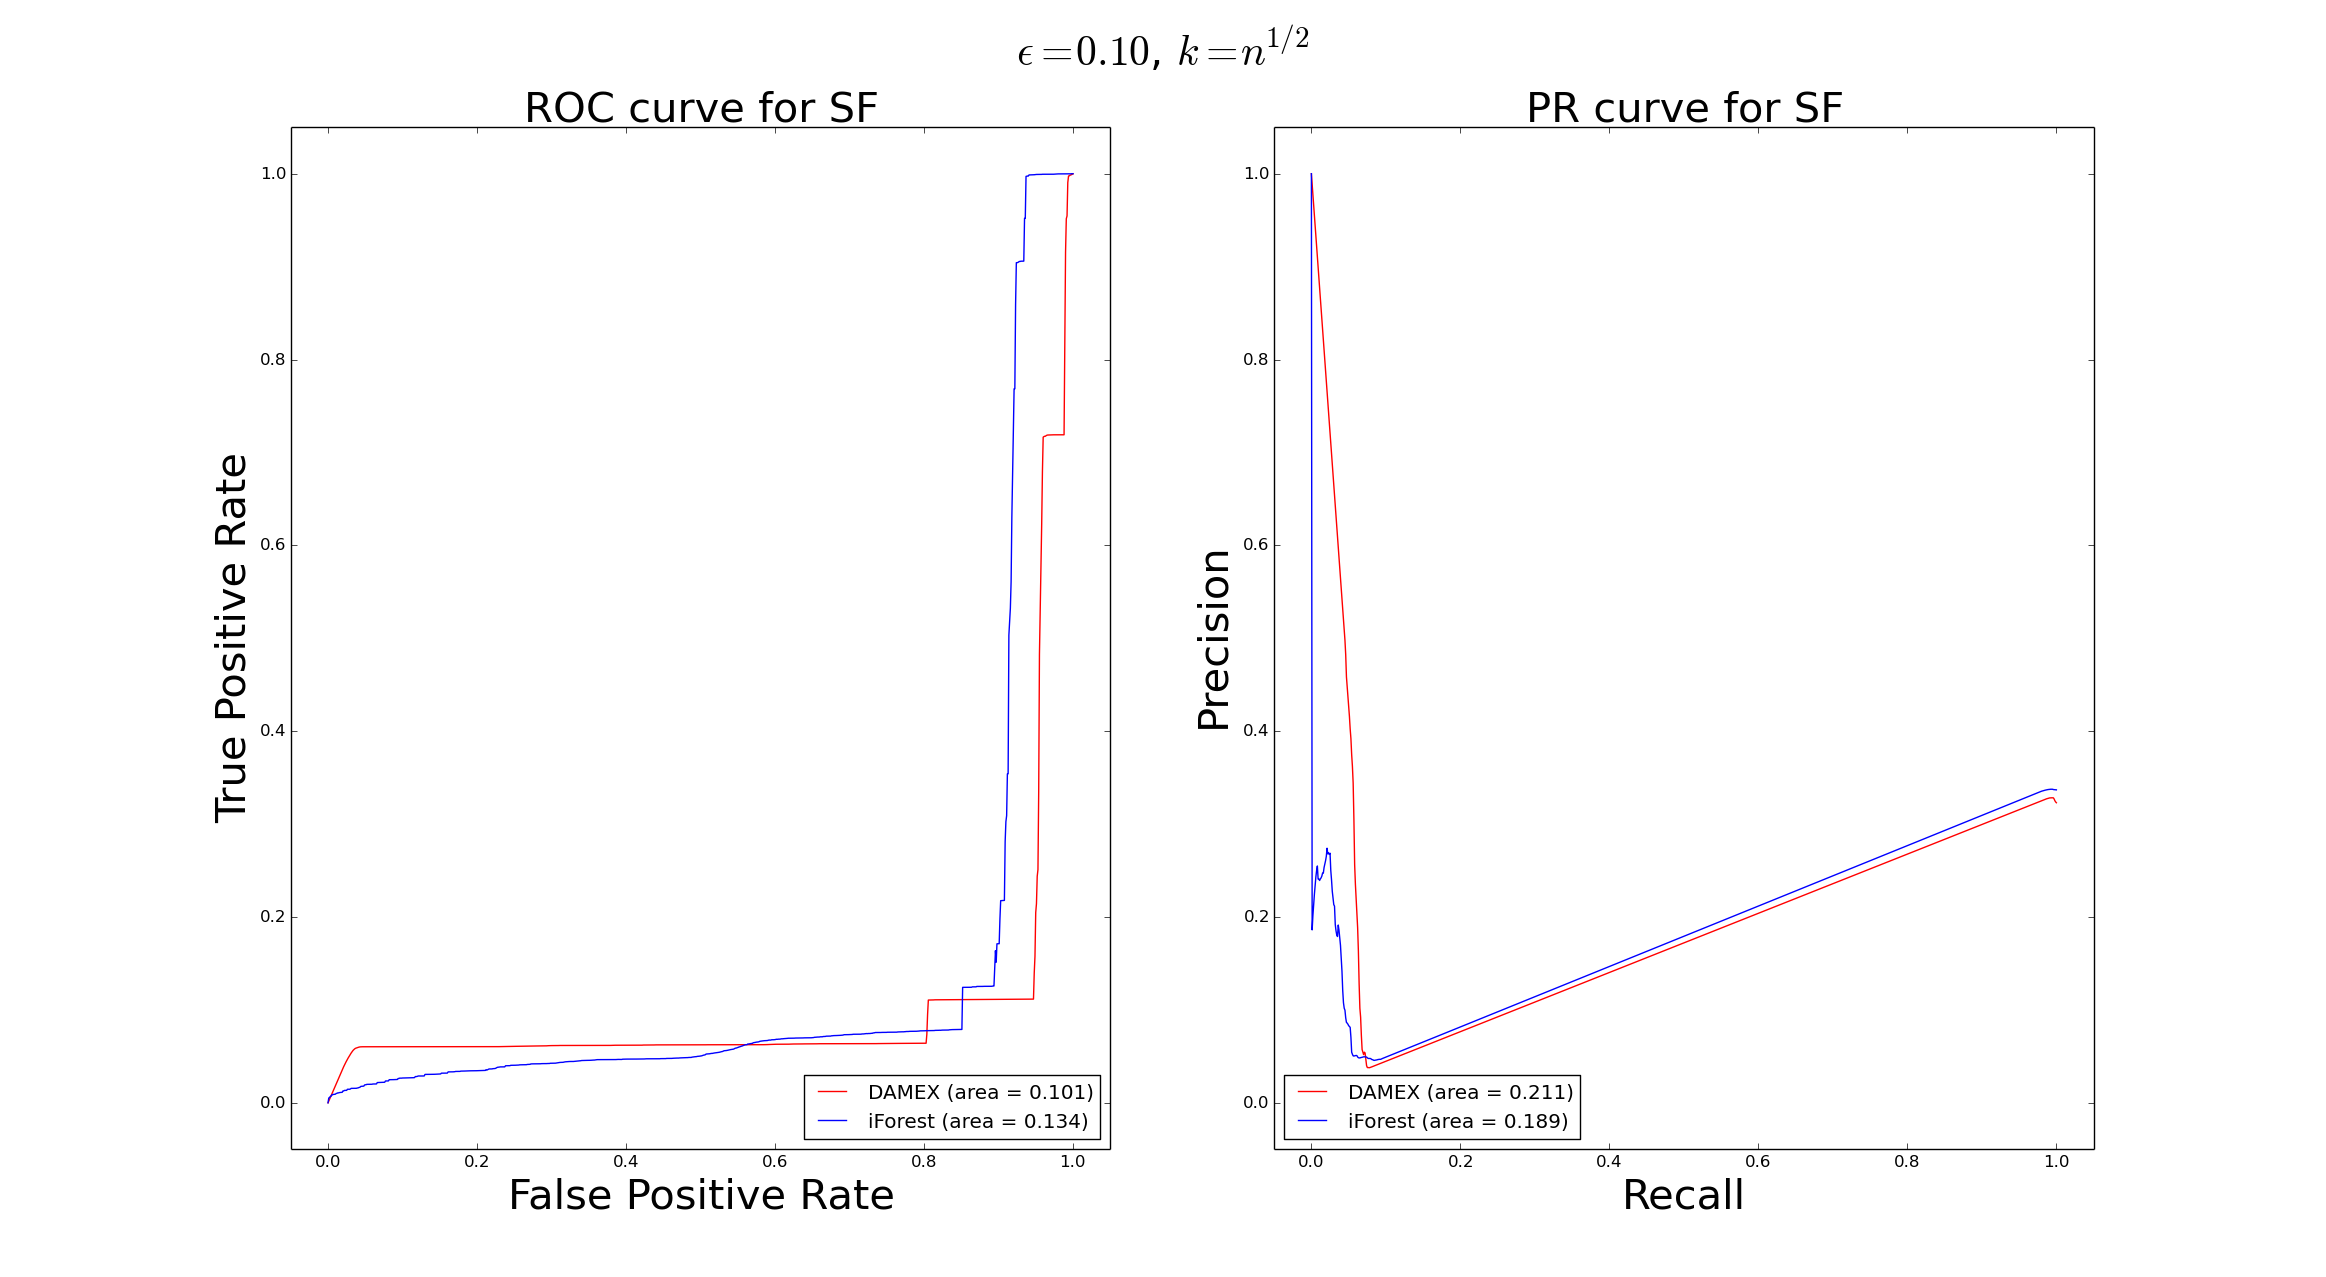
\includegraphics[width = \textwidth]{fig_source/SF-4d-lb-semi-supervised-average-rect-1}
  \caption{SF dataset, larger $\epsilon$}
\label{jmva:fig:SF_1}
\end{figure}

Considering the significant performance improvements on extreme data,
DAMEX may be combined with any standard anomaly detection algorithm to handle extreme
\emph{and} non-extreme data. This would improve the \emph{global}
performance of the chosen standard algorithm, and in particular
decrease the false alarm rate (increase the slope of the ROC curve's tangents near
the origin).  This combination can be done % as illustrated in
% Fig.~\ref{jmva:fig:combination}
by splitting the input space between an
extreme region and a non-extreme one, then using
Algorithm~\ref{jmva:DAMEX-algo} to treat new observations that appear in
the extreme region, and the standard algorithm to deal with those which
appear in the non-extreme region.  % The challenge is then to dovetail
% the two scoring functions obtained, restricted to different
% regions. One way to do it, is to re-scale the scoring function on the
% extreme region from DAMEX, to the (unused) one from the standard
% algorithm on the same region.

% \begin{figure}[!ht]
% \centering
% \includegraphics[scale=0.4]{extreme_AD}
% \caption{Combination of any AD algorithm with DAMEX}
% \label{jmva:fig:combination}
% \end{figure}

\begin{figure}[!ht]
  \centering
  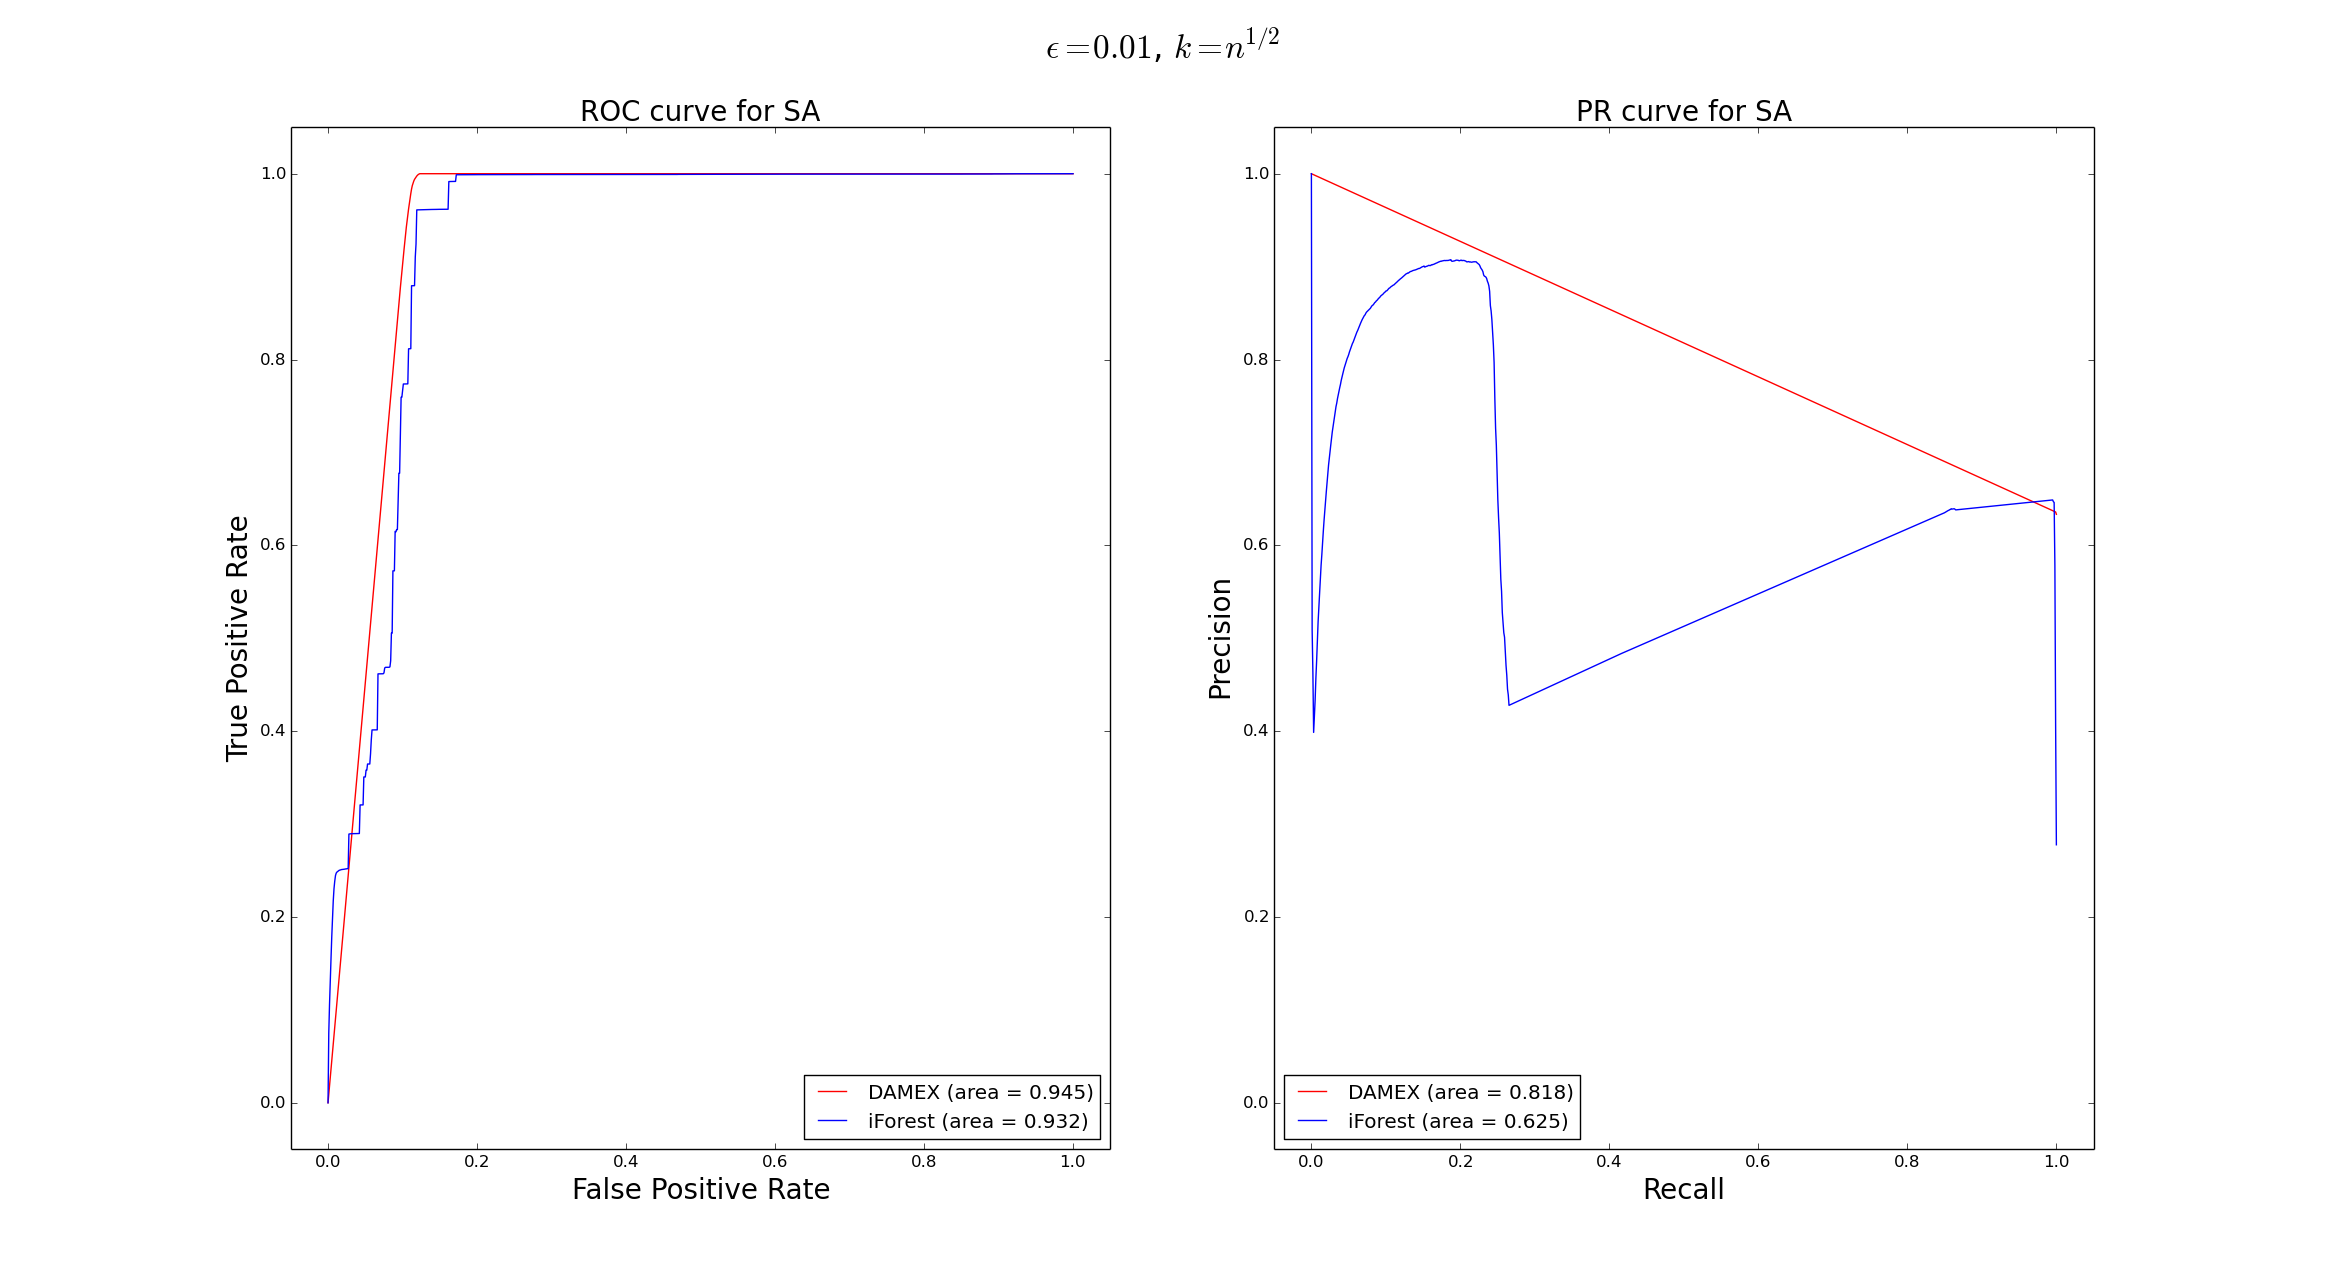
\includegraphics[width = \textwidth]{fig_source/SA-lb-semi-supervised-average-rect-01.png}
  \caption{SA dataset, default parameters}
  \label{jmva:fig:SA}
\end{figure}

\begin{figure}[!ht]
  \centering
  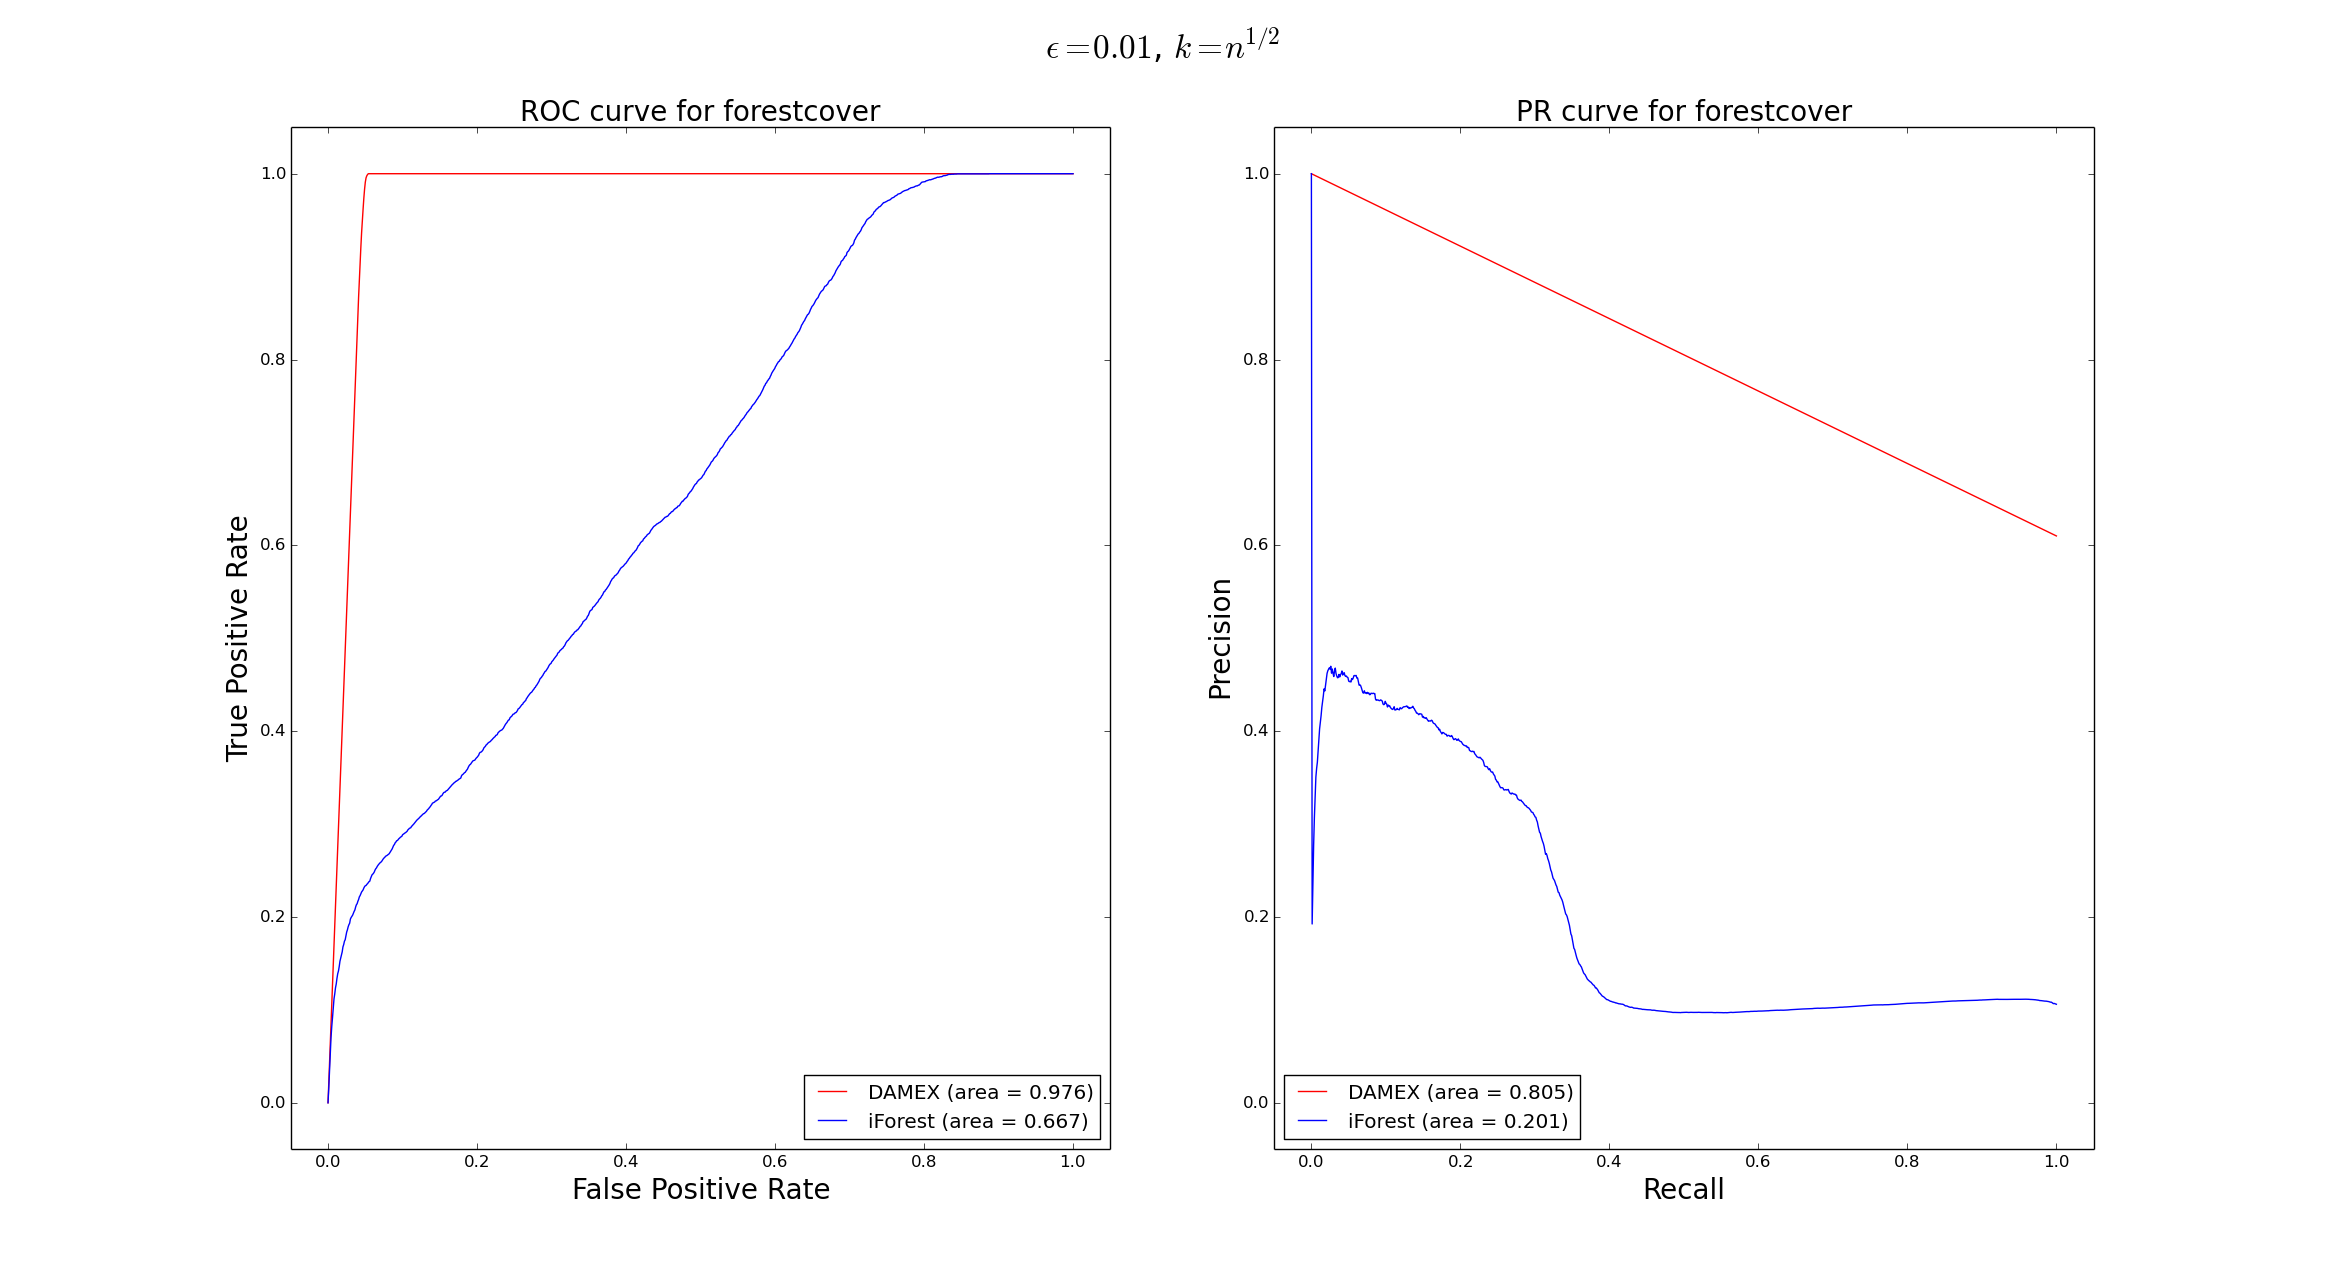
\includegraphics[width = \textwidth]{fig_source/forestcover-semi-supervised-average-rect-01.png}
  \caption{forestcover dataset, default parameters}
\label{jmva:fig:forestcover}
\end{figure}

\begin{figure}[!ht]
  \centering
  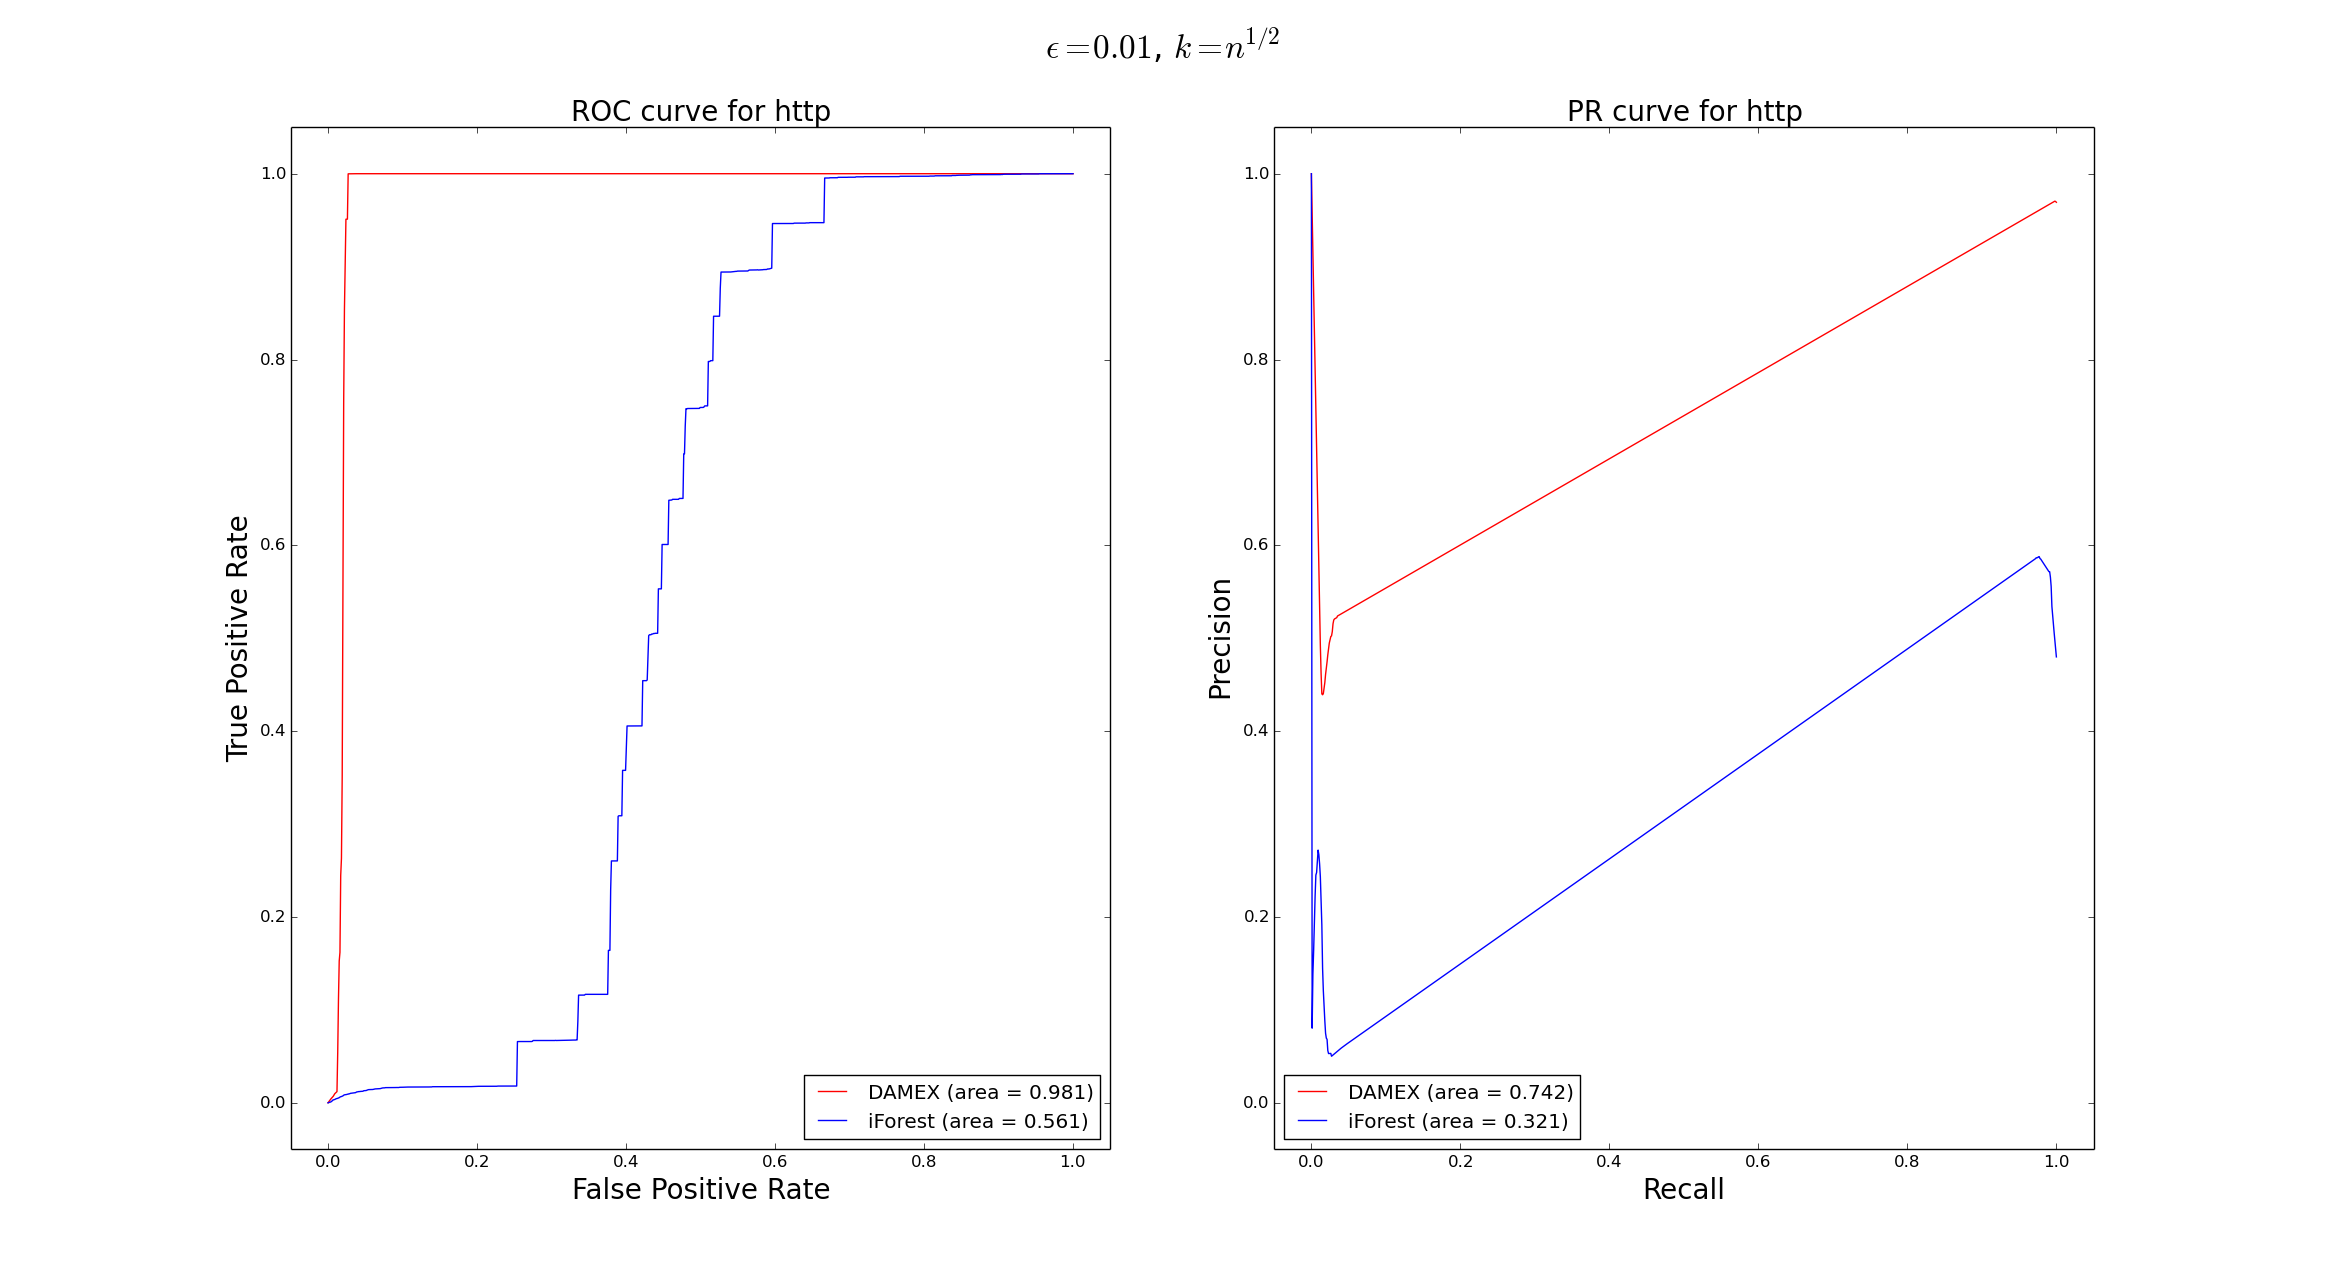
\includegraphics[width = \textwidth]{fig_source/http-3d-semi-supervised-average-rect-01.png}
  \caption{http dataset, default parameters}
\label{jmva:fig:http}
\end{figure}

\section{Conclusion}
The contribution of this chapter is twofold. First, it brings advances in multivariate EVT by designing a statistical method that possibly exhibits a sparsity pattern in the dependence structure of extremes, while deriving non-asymptotic bounds to assess the accuracy of the estimation procedure. Our method is intended to be used as a preprocessing step to scale up multivariate extreme values modeling to high dimensional settings, which is currently one of the major challenges in multivariate EVT.
Since the asymptotic bias ($\text{bias}(\alpha,n,k, \epsilon)$ in eq.~\eqref{jmva:eq:bias}) appears as a separate term  in the bound established, no second order
assumption is required. One possible line of further research would be to make  such an assumption (\ie\,to assume that the bias itself is regularly varying), in order to choose $\epsilon$ in an adaptive way with respect to $k$ and $n$ (see Remark~\ref{jmva:rk_param_choice}). This might also open up the possibility of de-biasing the estimation procedure (\cite{Fougeres2015}, \cite{Beirlant2015}). 
As a second contribution, this work extends the applicability of multivariate  EVT to the field of anomaly detection: a multivariate EVT-based algorithm which scores extreme observations according to their degree of abnormality is proposed. Due to its moderate complexity  --of order $d n \log n$--  this algorithm is suitable for the treatment of real word large-scale learning problems, and experimental results reveal a significantly increased performance on extreme regions compared with standard anomaly detection approaches.

%% The Appendices part is started with the command \appendix;
%% appendix sections are then done as normal sections
 
\section{Technical proofs}
\label{jmva:appendix_proof}
\subsection{Proof of Lemma \ref{jmva:lem:equivalence}}
For $n$ vectors $\mb v_1,\ldots,\mb v_n$ in $\mathbb{R}^d$, let us denote by $rank(v_i^j)$ the rank of $v_i^j$ among $v_1^j,\ldots,v_n^j$, that is $rank(v_i^j)=\sum_{k=1}^n \mathds{1}_{\{v_k^j \le v_i^j\}}$, so that $\hat F_j(X_i^j) = (rank(X_i^j)-1)/n$. For the first equivalence, notice that $\hat V_i^j = 1 / \hat U_i^j$.
For the others, we have both at the same time:
\begin{align*}
\hat V_i^j \ge \frac{n}{k} x_j  &~~\Leftrightarrow~~ 1-\frac{rank(X_i^j)-1}{n} ~\le~ \frac{k}{n}~x_j^{-1} 
\\ &~~\Leftrightarrow~~ rank(X_i^j) \ge n-kx_j^{-1} + 1 
\\ &~~\Leftrightarrow~~ rank(X_i^j) \ge n-\lfloor kx_j^{-1}\rfloor + 1 
\\ &~~\Leftrightarrow~~ X_i^j \ge X_{(n-\lfloor kx_j^{-1}\rfloor +1)}^j, 
\end{align*}
and
\begin{align*}
& X_i^j \ge X_{(n-\lfloor  kx_j^{-1} \rfloor +1)}^j ~\Leftrightarrow~
 rank(X_i^j) \ge n-\lfloor  kx_j^{-1} \rfloor+1 \\
&~~~~~~~~~~~~~~~~\Leftrightarrow~  rank( F_j(X_i^j)) \ge n-\lfloor
 kx_j^{-1}\rfloor+1 \qquad(\text{with probability one})\\ 
&~~~~~~~~~~~~~~~~\Leftrightarrow~  rank(1-F_j(X_i^j)) \le \lfloor kx_j^{-1}\rfloor\\
&~~~~~~~~~~~~~~~~\Leftrightarrow~  U_i^j \le U_{(\lfloor kx_j^{-1}\rfloor)}^j.
\end{align*}


\subsection{Proof of Lemma \ref{jmva:lem:g-alpha}}
% First of all, denoting by $A_t$ the event $\bigcap_{j \in \alpha} \left\{ U^j \le t x_j \right\}$ we have:
% \begin{align*}
% \tilde F_{\alpha, \beta} (t \mb x, t \mb z) &~=~ \mathbb{P} \left[ A_t ~~\bigcap~~ \left\{t z_j < U^j  ~~\text{ for } j \in\beta \right\}\right]\\
% &~=~\mathbb{P} \left[ A_t \right] 
% - \mathbb{P} \left[ A_t ~~\bigcap~~ \bigcup_{j \in\beta} \left\{U^j \le t z_j  \right\}\right]
% \end{align*}
% and
% \begin{align*}
% t^{-1}\mathbb{P} \left[ A_t \right] &~~\to~~ \mu\left[\bigcap_{j \in \alpha}\{u,~x_j^{-1} \le u_j\}\right]\\
% t^{-1} \mathbb{P} \left[ A_t ~~\bigcap~~ \bigcup_{j \in\beta} \left\{U^j \le t z_j  \right\}\right]
% &~~\to~~ \mu\left[\bigcap_{j \in \alpha}\{u,~x_j^{-1} \le u_j\} ~~\bigcap~~ \bigcup_{j \in\beta}\{u,~z_j^{-1} \le u_j\}\right]~.
% \end{align*}
% Now, if we denote by $T$ the transformation to polar coordinates, namely $T(u)=(R(u), \Theta(u))$ with $R(u):= \|u\|_\infty$ and $\Theta (u):= \left( \frac{u_1}{R(u)},..., \frac{u_d}{R(u)} \right)$, then
% \begin{align*}
% T \left( \bigcap_{j \in \alpha} \left\{ u,~x_j^{-1} \le u_j\right\} \right) &=  \bigcap_{j \in \alpha}\left\{(r, w),~(w_j x_j)^{-1} \le r \right\} \\
% & =  \left\{ (r, w), ~ \bigvee_{j \in \alpha} (w_j x_j)^{-1} \le r \right\}
% \end{align*}
% so that 
% \begin{align*}
% \mu\left[\bigcap_{j \in \alpha}\left\{u,~x_j^{-1} \le u_j\right\}\right] &= \mu \circ T ^{-1} \left\{(r, w), ~ \bigvee_{j \in \alpha} (w_j x_j)^{-1} \le r \right\} \\
% &= \left( r^{-2}dr \phi \right)  \left\{(r, w), ~ \bigvee_{j \in \alpha} (w_j x_j)^{-1} \le r \right\}\\
% &= \int_{w \in S^{d-1}} \left( \bigvee_{j \in \alpha} (w_j x_j)^{-1} \right)^{-1} \phi(dw)\\
% &= \int_{w \in S^{d-1}}~ \bigwedge_{j \in \alpha} (w_j x_j)~ \phi(dw)~.
% \end{align*}
% Of an analoguous manner we may write:
% \begin{align*}
% &\mu\left[\bigcap_{j \in \alpha}\{u,~x_j^{-1} \le u_j\} ~~\bigcap~~ \bigcup_{j \in\beta}\{u,~z_j^{-1} \le u_j\}\right] \\
% &~~~~~~~~~~~~~~~~~~~~~~~~~~~~~~~=  \mu \circ T ^{-1} \left\{(r, w), ~ \bigvee_{j \in \alpha} (w_j x_j)^{-1} \le r ~~\text{and}~~ \bigwedge_{j \in\beta} (w_j z_j)^{-1} \le r\right\}\\
% &~~~~~~~~~~~~~~~~~~~~~~~~~~~~~~~= \left( r^{-2}dr \phi \right) \left\{(r, w), ~ \max \left( \bigvee_{j \in \alpha} (w_j x_j)^{-1}~,~\bigwedge_{j \in\beta} (w_j z_j)^{-1} \right) \le r\right\}\\
% &~~~~~~~~~~~~~~~~~~~~~~~~~~~~~~~= \int_{w \in S^{d-1}} \left( \max \left( \bigvee_{j \in \alpha} (w_j x_j)^{-1}~,~\bigwedge_{j \in\beta} (w_j z_j)^{-1} \right) \right)^{-1} \phi(dw)\\
% &~~~~~~~~~~~~~~~~~~~~~~~~~~~~~~~= \int_{w \in S^{d-1}} \min \left( \left(\bigvee_{j \in \alpha} (w_j x_j)^{-1}\right)^{-1}~,~\left(\bigwedge_{j \in\beta} (w_j z_j)^{-1}\right)^{-1} \right)  \phi(dw)\\
% &~~~~~~~~~~~~~~~~~~~~~~~~~~~~~~~= \int_{w \in S^{d-1}} \min \left( \bigwedge_{j \in \alpha} w_j x_j~,~\bigvee_{j \in\beta} w_j z_j \right)  \phi(dw)\\
% \end{align*}
% We then obtain:
% \begin{align*}
% g_\alpha(x) = \int_{S^{d-1}} \bigwedge_{j \in \alpha}{w_j x_j}~ \phi(dw) - \int_{S^{d-1}} \min \left(\bigwedge_{j \in \alpha}{w_j x_j}~,~ \bigvee_{j \in\beta} w_j z_j\right) \phi(dw)
% \end{align*}

First, recall that $g_{\alpha,\beta}(\mb x,\mb z) = \mu\big( R(\mb x^{-1},\mb z^{-1}, \alpha,\beta)\big)$, see \eqref{jmva:g_with_mu}. %(this is also valid if some $\alpha_i = 1$, with the convention $\alpha_i^{-1} = +\infty$ is $\alpha = 0$). 
Denote by $\pi$ the transformation to pseudo-polar coordinates introduced
in Section~\ref{jmva:sec:framework}, 
\[
\begin{aligned}
  \pi: [0,\infty]^d \setminus\{\mb 0\} &\to  (0,\infty]\times S^{d-1}_\infty \\
\mb v & \mapsto (r,\boldsymbol{\theta}) = (\|\mb v\|_\infty, \|\mb v\|_\infty^{-1} \mb v). 
\end{aligned}
\]
Then, we have $\ud (\mu \circ\pi^{-1})= \frac{\ud r}{r^2}\ud
\Phi$ on $(0,\infty]\times S^{d-1}_\infty$. This classical result from EVT
comes from the fact that, for $r_0>0$ and $B\subset S^{d-1}_\infty$,  $\mu\circ\pi^{-1}\{ r\ge r_0, \boldsymbol{\theta}\in B\}
= r_0^{-1}\Phi(B)$, see \eqref{jmva:mu-phi}.
Then 
\[
\begin{aligned}
 g_{\alpha,\beta}(\mb x,\mb z)  & = 
\mu\circ\pi^{-1}\Big\{(r,\boldsymbol{\theta}): \quad \forall i \in\alpha,~ r \theta_i \ge
x_i^{-1}\;; \quad \forall j \in\beta, r \theta_j < z_j^{-1} \Big\} \\
&= \mu \circ \pi^{-1} \Big\{(r,\boldsymbol{\theta}): \quad  r  \ge \bigvee_{i\in\alpha}
(\theta_ix_i)^{-1}\;; \quad  r  <\bigwedge_{j\in\beta}(\theta_j z_j)^{-1} \Big\} \\
&= \int_{\boldsymbol{\theta}\in S^{d-1}_\infty} \int_{r>0} \mathds{1}_{r  \ge \bigvee_{i\in\alpha}
(\theta_ix_i)^{-1}}\;\mathds{1}_{r  <\bigwedge_{j\in\beta}(\theta_j
z_j)^{-1}} \frac{\ud r}{r^2} \ud \Phi(\boldsymbol{\theta}) \\ 
& = \int_{\boldsymbol{\theta}\in S^{d-1}_\infty}  \left(
\Big(\bigvee_{i\in\alpha} (\theta_ix_i)^{-1}\Big)^{-1}  - 
\Big(  \bigwedge_{j\in\beta}(\theta_jz_j)^{-1} \Big)^{-1} \right)_+
\ud \Phi(\boldsymbol{\theta}) \\ 
& = \int_{\boldsymbol{\theta}\in S^{d-1}_\infty}  \left(
\bigwedge_{i\in\alpha} \theta_ix_i   - 
 \bigvee_{j\in\beta}\theta_jz_j  \right)_+ \ud \Phi(\boldsymbol{\theta}), \\ 
\end{aligned}
\]
which proves the first assertion. 
To prove the Lipschitz property, notice first that, 
for any finite sequence of real numbers  $c$ and $d$,
$\max_i c_i - \max_i d_i \le \max_i (c_i - d_i)$ and $\min_i c_i -
\min_i d_i \le \max_i (c_i - d_i)$. 
Thus for every $\mb x, \mb z \in [ 0, \infty]^d \setminus \{\boldsymbol{\infty}\}$ and $\theta \in S_\infty^{d-1}$:
\begin{align*}
  &\left(\bigwedge_{j \in \alpha}{\theta_j x_j} - \bigvee_{j \in\beta} \theta_j z_j\right)_+ - \left(\bigwedge_{j \in \alpha}{\theta_j x_j'} - \bigvee_{j \in\beta} \theta_j z_j'\right)_+ \nonumber\\
  &~~~~~~~~~~~~~~~~~~~~~~~~~~~~\le~
 \left[\left(\bigwedge_{j \in \alpha}{\theta_j x_j} -
      \bigvee_{j \in\beta} \theta_j z_j\right) - \left(\bigwedge_{j
        \in \alpha}{\theta_j x_j'} - \bigvee_{j \in\beta} \theta_j
      z_j'\right)\right]_+ \nonumber\\
&~~~~~~~~~~~~~~~~~~~~~~~~~~~~\le~
\left[\bigwedge_{j \in \alpha}{\theta_j x_j} - \bigwedge_{j \in
  \alpha}{\theta_j x_j'} ~+~ \bigvee_{j \in\beta} \theta_j z_j' -
\bigvee_{j \in\beta} \theta_j z_j\right]_+\nonumber\\
&~~~~~~~~~~~~~~~~~~~~~~~~~~~~\le~
    \left[\max_{j \in \alpha}(\theta_j x_j - \theta_j x_j')
      ~+~ \max_{j \in\beta} (\theta_j z_j' - \theta_j z_j) \right]_+ \\%\label{jmva:eq:resultGalpha}\\
 &~~~~~~~~~~~~~~~~~~~~~~~~~~~~\le~
\max_{j \in \alpha}\theta_j|{ x_j} - { x_j'}| ~+~ \max_{j \in\beta} \theta_j | z_j' -  z_j|
\end{align*}
Hence,
\begin{align*}
&|g_{\alpha,\beta}(\mb x, \mb z) - g_{\alpha,\beta}(\mb x', \mb z')|\\
% &~~~~~~~~~~~~~~~~~~~~~~\le~ \int_{S^{d-1}_\infty} \left(\max_{j \in \alpha}|{\theta_j x_j} -
%   {\theta_j x_j'}| ~+~ \max_{j \in\beta} |\theta_j z_j' - \theta_j
%   z_j|\right) \ud \Phi(\boldsymbol{\theta}). \\
&~~~~~~~~~~~~~~~~~~~~~~~\le~\int_{S^{d-1}_\infty} \left(\max_{j \in \alpha}\theta_j|{ x_j} - { x_j'}| ~+~ \max_{j \in\beta} \theta_j | z_j' -  z_j|\right)  \ud\Phi(\boldsymbol{\theta})~.
\end{align*}
Now, by \eqref{jmva:eq:integratePhiLambda} we have:
$$\int_{S^{d-1}_\infty} \max_{j \in \alpha}\theta_j|{ x_j} - { x_j'}| ~~ \ud\Phi(\boldsymbol{\theta}) = \mu([\mb 0, \mb{\tilde x}^{-1}]^c)$$ with $\mb{\tilde x}$ defined as $\tilde x_j = |x_j - x_j'|$ for $j\in\alpha$, and $0$ elsewhere.
It suffices then to write:
\begin{align*}
\mu([\mb 0, \mb{\tilde x}^{-1}]^c) &= \mu(\{y,~\exists j \in \alpha,~y_j \ge |x_j-x_j'|^{-1}\})\\
 &\le \sum_{j\in\alpha}\mu(\{y,~y_j \ge |x_j-x_j'|^{-1}\})\\
 &\le \sum_{j \in \alpha} |x_j-x_j'|~.
\end{align*}
Similarly, $\int_{S^{d-1}_\infty} \max_{j \in\beta} \theta_j | z_j' -  z_j|  ~~ \ud\Phi(\boldsymbol{\theta}) ~\le~ \sum_{j \in \beta} |z_j-z_j'|$.

%
% Now, following
% the same argument as that leading to (\ref{jmva:eq:resultGalpha}), one obtains that $\mu\{ \mb v: v_j\ge 1\}  =
% \int_{S^{d-1}_\infty} \theta_j \ud\Phi(\boldsymbol{\theta})$.
% Since our marginal standardization choice  implies $\mu\{\mb v:
% v_j\ge 1\} = 1$, we get that 
% \begin{align*}
% |g_{\alpha,\beta}(\mb x, \mb z) - g_{\alpha,\beta}(\mb x', \mb z')|\le\|\mb x - \mb x'\|_\infty + \|\mb z - \mb z'\|_\infty ~\le \|\mb x - \mb x'\|_1 + \|\mb z - \mb z'\|_1.
% \end{align*}


\subsection{Proof of Proposition \ref{jmva:prop:g}}
%For notational convenience, we denote by $\max_\alpha$ the maximum taken on $\{\alpha \subset \{1,...d\} \setminus \emptyset \}$.
The starting point is inequality (9) on p.7 in \cite{COLT15} which bounds the deviation of the empirical measure on extreme regions. 
%Consider a random vector $\mathbf{Z}=(Z^1,\ldots,Z^d)$ with uniform margins on $[0,1]$,
Let $\mathcal{C}_n(\point)=\frac{1}{n} \sum_{i=1}^{n} \mathds{1}_{\{\mb Z_i \in \point \}}$ 
% (the $\mb Z_i$'s are \iid~realizations of $\mb Z$ )
and $\mathcal{C}(\mathbf{x})=\mathbb{P}(\mb Z \in \point)$ be the empirical and true measures associated with a n-sample $\mb Z_1, \ldots, \mb Z_d$ of \iid~realizations of a random vector $\mathbf{Z}=(Z^1,\ldots,Z^d)$ with uniform margins on $[0,1]$. Then for any real number $\delta \ge e^{-k}$, 
with probability greater than $1 - \delta$,
\begin{align}
\label{jmva:Qialt2}
\sup_{0 \le \mathbf{x} \le T} \frac{n}{k} \left | \mathcal{C}_n(\frac{k}{n} [\mathbf{x},\boldsymbol{\infty}[^c) - \mathcal{C}(\frac{k}{n} [\mathbf{x},\boldsymbol{\infty}[^c)  \right| ~\le~ C d\sqrt{\frac{T}{k} \log{\frac{1}{\delta}}}~.
\end{align} 
Recall that with the above notations, $0 \le \mb x \le T$ means $0 \le x_j \le T$ for every $j$.
The proof of Proposition~\ref{jmva:prop:g} follows the same lines as in \cite{COLT15}. 
The cornerstone concentration inequality \eqref{jmva:Qialt2} has to be replaced with 
\begin{align}
\label{jmva:cornerstone-extension}
\nonumber \max_{\alpha, \beta} \sup_{\substack{  0 \le \mb x, \mb z \le T \\ \exists j \in \alpha, x_j \le T'}}
&\frac{n}{k} \left | \mathcal{C}_n \left(\frac{k}{n} R(\mb x^{-1}, \mb z^{-1}, \alpha,~\beta)^{-1}\right) - \mathcal{C}\left(\frac{k}{n} R(\mb x^{-1}, \mb z^{-1}, \alpha,~\beta)^{-1}\right)  \right|\\
&~~~~~~~~~~~~~~~~~~~~~~~~~~~~~~~~~~~~~~~~~ ~\le~ Cd \sqrt{\frac{dT'}{k} \log{\frac{1}{\delta}}}~.
\end{align}
\begin{remark}
Inequality \eqref{jmva:cornerstone-extension} is here written in its full generality, namely with a separate constant $T'$ possibly smaller than $T$. If $T' < T$, we then have a smaller bound (typically, we may use $T = 1/\epsilon$ and $T' = 1$). However, we only use \eqref{jmva:cornerstone-extension} with $T = T'$ in the analysis below, since the smaller bounds in $T'$ obtained (on $\Lambda(n)$ in \eqref{jmva:proof_decomp}) would be diluted (by $\Upsilon(n)$ in \eqref{jmva:proof_decomp}).
\end{remark}
\begin{proof}[Proof of (\ref{jmva:cornerstone-extension})]
Recall that for notational convenience we write `$\alpha,\beta$' for `$\alpha$ non-empty subset of $ \{1,\ldots,d\}$ and $\beta$ subset of $ \{1,\ldots,d\}$'.
% Inequality \eqref{jmva:cornerstone-extension} is obtained by using
The key is to apply Theorem 1 in \cite{COLT15}, with a VC-class which fits our purposes. Namely, consider
\begin{align*}
\mathcal{A} ~~=~~ \mathcal{A}_{T,T'} ~~&=~~ \bigcup_{\alpha, \beta} \mathcal{A}_{T,T',\alpha,\beta} \text{~~~~~with}\\
\mathcal{A}_{T,T',\alpha,\beta} ~~=~~& \frac{k}{n}\Big\{ R(\mb x^{-1}, \mb z^{-1}, \alpha,~\beta)^{-1}:~~ \mb x, \mb z \in \mathbb{R}^d ,~ 0 \le \mb x, \mb z \le T,\\
&~~~~~~~~~~~~~~~~~~~~~~~~~~~~~~~~~~~~~~~~~~~~~~~~~~~~~~~~\exists j \in \alpha, x_j \le T' \Big\}~,
\end{align*}
for $T,~T' > 0$ and $\alpha,~\beta \subset \dd,~\alpha \neq \emptyset$. $\mathcal{A}$ has VC-dimension $V_\mathcal{A} = d$, as the one considered in \cite{COLT15}. Recall in view of (\ref{jmva:set-R}) that 
\begin{align*}
R(\mb x^{-1}, \mb z^{-1}, \alpha,~\beta)^{-1} ~&=~ \Big\{ \mb y \in [0, \infty]^d , ~~y_j \le x_j ~~\text{ for } j \in \alpha,\\
&~~~~~~~~~~~~~~~~~~~~~~~~~  y_j > z_j ~~\text{ for } j \in\beta ~~\Big\} \\&=~ [\mb a, \mb b],
\end{align*}
with $\mb a$ and $\mb b$ defined by 
$a_j =   \left \lbrace \begin{array}{cc}
0 &  \text{for} ~ j \in \alpha \\
z_j  & \text{for} ~ j \in\beta \\
\end{array}
\right.$
and
$b_j =   \left \lbrace \begin{array}{cc}
x_j &  \text{for} ~ j \in \alpha \\
\infty  & \text{for} ~ j \in\beta \\
\end{array}
\right.$.
Since we have $\forall A \in \mathcal{A}, A \subset [\frac{k}{n} \mb T',~\boldsymbol{\infty}[^c$, the probability for a \rv~$\mb Z$ with uniform margins in $[0,1]$ to be in the union class $\mathbb{A} = \bigcup_{A \in \mathcal{A}}A$ is $\mathbb{P}(\mb Z \in \mathbb{A}) \le \mathbb{P}(\mb Z \in [\frac{k}{n}\mb T',~\boldsymbol{\infty}[^c) \le \sum_{j=1}^d \mathbb{P}(Z^j \le \frac{k}{n} T') \le \frac{k}{n}dT'$. 
Inequality \eqref{jmva:cornerstone-extension} is thus a direct consequence of Theorem 1 in \cite{COLT15}.
\end{proof}
\noindent
Define now the empirical version $\tilde F_{n, \alpha, \beta}$ of $\tilde F_{\alpha, \beta}$ (introduced in (\ref{jmva:F-tilde-alpha})) as 
\begin{align}
\label{jmva:def:Fn}
\tilde F_{n, \alpha, \beta}(\mb x, \mb z)  ~=~ \frac{1}{n} \sum_{i=1}^n \mathds{1}_{\{ U_i^j \le x_j ~~\text{for}~ j \in \alpha ~~\text{ and }~~  U_i^j > z_j ~~\text{for}~ j \in\beta \}}~ ,
\end{align}
so that 
$  \frac{n}{k} \tilde F_{n, \alpha, \beta}( \frac{k}{n} \mb x, \frac{k}{n} \mb z) ~=~ \frac{1}{k} \sum_{i=1}^n 
\mathds{1}_{\{ U_i^j \le \frac{k}{n} x_j ~~\text{for}~ j \in \alpha ~~\text{ and }~~ U_i^j > \frac{k}{n} z_j   ~~\text{for}~ j \in\beta \}}.$
Notice that the $U_i^j$'s are  not observable (since $F_j$ is
unknown). In fact, $\tilde F_{n, \alpha, \beta}$ will be used as a substitute for $g_{n, \alpha, \beta}$ (defined in \eqref{jmva:def:gn}) allowing to handle uniform variables. This is illustrated by the following lemmas. 

\begin{lemma}[Link between $g_{n, \alpha, \beta}$ and $\tilde F_{n, \alpha, \beta}$]
\label{jmva:lem:gn-Fn}
The  empirical version of $\tilde F_{\alpha, \beta}$ and that of $g_{\alpha, \beta}$ are related \emph{via}
\begin{align*}
g_{n, \alpha, \beta}(\mb x, \mb z)~=~\frac{n}{k} \tilde F_{n, \alpha, \beta}\left( \left(U_{(\lfloor kx_j\rfloor)}^j\right)_{j \in \alpha} , \left(U_{(\lfloor kz_j\rfloor)}^j\right)_{j \in \beta}\right),
\end{align*}
\end{lemma}

\begin{proof}
Considering the definition in (\ref{jmva:def:Fn}) and (\ref{jmva:eq:gn2}), both sides are equal to $\mu_n(R(\mathbf{x}^{-1}, \mathbf{z}^{-1}, \alpha,\beta))$. %by Lemma \ref{jmva:lem:equivalence}.
\end{proof}


\begin{lemma}[Uniform bound on $\tilde F_{n, \alpha, \beta}$'s deviations]
\label{jmva:lem:Fn-tildeF}
 For any finite  $T>0$, and $\delta\ge e^{-k}$,  with probability at least $1-\delta$, the  deviation of $\tilde F_{n, \alpha, \beta}$ from  $\tilde F_{\alpha, \beta}$ is uniformly bounded: % independently of $\alpha$ and $\beta$:
 
\begin{align*}
\max_{\alpha, \beta} \sup_{ 0 \le \mb x, \mb z \le T}
\left| \frac{n}{k} \tilde F_{n, \alpha, \beta}( \frac{k}{n} \mb x, \frac{k}{n} \mb z)-\frac{n}{k} \tilde F_{\alpha, \beta}( \frac{k}{n} \mb x, \frac{k}{n} \mb z) \right| \le Cd\sqrt{\frac{T}{k}\log{\frac{1}{\delta}}}~.
\end{align*}
\end{lemma}
\begin{proof}
Notice that 
\begin{align*}
&\sup_{ 0 \le \mb x, \mb z \le T} \left| \frac{n}{k} \tilde F_{n, \alpha, \beta}( \frac{k}{n} \mb x, \frac{k}{n} \mb z)- \frac{n}{k} \tilde F_{\alpha, \beta}( \frac{k}{n} \mb x, \frac{k}{n} \mb z) \right|  \\
&~= \sup_{ 0 \le \mb x, \mb z \le T} \frac{n}{k} \left|  \frac{1}{n}  \sum_{i=1}^n \mathds{1}_{ \mb U_i \in \frac{k}{n} R(\mb x^{-1}, \mb z^{-1}, \alpha,~\beta)^{-1} } -
   \mathbb{P} \left[ \mathbf{U} \in \frac{k}{n} R(\mb x^{-1}, \mb z^{-1}, \alpha,~\beta)^{-1}
   \right] \right|,
\end{align*}
and apply inequality (\ref{jmva:cornerstone-extension}) with $T'=T$.
\end{proof}
%
\begin{remark}
%\label{jmva:rk:prop:g_generalized}
\label{jmva:rk:lem:Fn-tildeF_generalized}
% For each $n>0$, with probability at least $1 - \delta$,~ for each $\alpha \subset\{1,\ldots,d\}\setminus \emptyset$ and $\beta \subset\{1,\ldots,d\}$,
% \begin{align*}
% \sup_{\substack{  0 \le \mb x, \mb z \le T \\ \exists j \in \alpha, x_j \le T'}} \left| g_{n, \alpha, \beta}(\mb x, \mb z) - g_{\alpha, \beta}(\mb x, \mb z) \right| &~\le~  Cd\sqrt{\frac{2T'}{k}\log\frac{d+3}{\delta}} 
% \\\nonumber &~~~~~~+ \sup_{0 \le \mb x, \mb z \le 2T}\left|\frac{n}{k} \tilde F_{\alpha, \beta}( \frac{k}{n} \mb x, \frac{k}{n} \mb z)- g_{\alpha, \beta}(\mb x, \mb z)\right|.
% \end{align*}
Note that the following stronger inequality holds true, when using (\ref{jmva:cornerstone-extension}) in full generality, \ie~with $T'< T$.
 For any finite  $T, T'>0$, and $\delta\ge e^{-k}$,  with probability at least $1-\delta$,
\begin{align*}
\max_{\alpha, \beta} \sup_{\substack{  0 \le \mb x, \mb z \le T \\ \exists j \in \alpha, x_j \le T'}}
\left| \frac{n}{k} \tilde F_{n, \alpha, \beta}( \frac{k}{n} \mb x, \frac{k}{n} \mb z)-\frac{n}{k} \tilde F_{\alpha, \beta}( \frac{k}{n} \mb x, \frac{k}{n} \mb z) \right| \le Cd\sqrt{\frac{T'}{k}\log{\frac{1}{\delta}}}.
\end{align*}
\end{remark}

The following lemma is stated and proved in \cite{COLT15}.
\begin{lemma}[Bound on the order statistics of $\mb U$]
\label{jmva:lem:U-x} 
Let $\delta\ge e^{-k}$. For any finite positive number $T>0$ such that $T \ge 7/2((\log d)/k + 1)$, we have with probability greater than $1 - \delta$, 
\begin{align}
\label{jmva:lem:eq-Wellner}
\forall~ 1\le j \le d,~~~~~\frac{n}{k} U_{(\lfloor kT\rfloor )}^j ~\le~ 2T~,
\end{align}
and with probability greater than $1- (d+1)\delta$, 
\begin{align*}
\max_{1 \le j \le d}~ \sup_{0 \le x_j \le T} \left| \frac{\lfloor kx_j\rfloor }{k} - \frac{n}{k} U_{(\lfloor kx_j\rfloor )}^j  \right| ~\le~ C\sqrt{\frac{T}{k}\log{\frac{1}{\delta}}}~.
\end{align*}
\end{lemma}
\noindent
We may now proceed with the proof of Proposition \ref{jmva:prop:g}.
Using Lemma \ref{jmva:lem:gn-Fn}, we may write:
\begin{align}
\nonumber &\max_{\alpha, \beta}\sup_{ 0 \le \mb x, \mb z \le T }
 \left| g_{n, \alpha, \beta}(\mb x, \mb z) - g_{\alpha, \beta}(\mb x, \mb z) \right| \\
\nonumber           &~~~~~~~~~~=~ \max_{\alpha, \beta}  \sup_{ 0 \le \mb x, \mb z \le T } \left| \frac{n}{k} \tilde F_{n, \alpha, \beta} \left( \left(U_{(\lfloor kx_j\rfloor)}^j\right)_{j \in \alpha} , \left(U_{(\lfloor kz_j\rfloor)}^j\right)_{j \in \beta} \right) - g_{\alpha, \beta}(\mb x, \mb z) \right| \\
\label{jmva:proof_decomp}&~~~~~~~~~~\le~ \Lambda(n) ~+~ \Xi(n) ~+~ \Upsilon(n)~.
\end{align}
with:
\begin{align*}
 \Lambda(n) &~=~ \max_{\alpha, \beta} \sup_{ 0 \le \mb x, \mb z \le T } \bigg| \frac{n}{k} \tilde F_{n, \alpha, \beta} \left(\left(U_{(\lfloor kx_j\rfloor)}^j\right)_{j \in \alpha} , \left(U_{(\lfloor kz_j\rfloor)}^j\right)_{j \in \beta} \right) 
\\&~~~~~~~~~~~~~~~~~~~~~~~~~~~~~~~~~~~~~~~- \frac{n}{k} \tilde F_{\alpha, \beta} \left(\left(U_{(\lfloor kx_j\rfloor)}^j\right)_{j \in \alpha} , \left(U_{(\lfloor kz_j\rfloor)}^j\right)_{j \in \beta} \right)  \bigg|\\
\Xi(n) &~=~\max_{\alpha, \beta} \sup_{0 \le \mb x, \mb z \le T} \bigg| \frac{n}{k} \tilde F_{\alpha, \beta} \left(\left(U_{(\lfloor kx_j\rfloor)}^j\right)_{j \in \alpha} , \left(U_{(\lfloor kz_j\rfloor)}^j\right)_{j \in \beta} \right)
\\&~~~~~~~~~~~~~~~~~~~~~~~~~~~~~~~~~~~~~- g_{\alpha, \beta}\left(\left(\frac{n}{k}U_{(\lfloor kx_j\rfloor)}^j\right)_{j \in \alpha} , \left(\frac{n}{k}U_{(\lfloor kz_j\rfloor)}^j\right)_{j \in \beta}\right) \bigg|\\
\Upsilon(n) &~=~ \max_{\alpha, \beta} \sup_{ 0 \le \mb x, \mb z \le T } \left| g_{\alpha, \beta}\left(\left(\frac{n}{k}U_{(\lfloor kx_j\rfloor)}^j\right)_{j \in \alpha} , \left(\frac{n}{k}U_{(\lfloor kz_j\rfloor)}^j\right)_{j \in \beta}\right) - g_{\alpha, \beta}(\mb x, \mb z) \right|.
\end{align*}
Now, considering (\ref{jmva:lem:eq-Wellner}) we have with probability greater than $1-\delta$ that
for every $1\le j \le d$, $U_{(\lfloor kT\rfloor )}^j ~\le~ 2T \frac{k}{n}~$, so that
\begin{align*} 
\Lambda(n) % &~\le~
% \max_{\alpha, \beta}  \sup_{ 0 \le \mb x, \mb z \le T } \bigg| \frac{n}{k} \tilde F_{n, \alpha, \beta}  \left(
% \left(U_{(\lfloor kx_j\rfloor)}^j\right)_{j \in \alpha} , \left(U_{(\lfloor kz_j\rfloor)}^j\right)_{j \in \beta} \right) 
% \\&~~~~~~~~~~~~~~~~~~~~~~~~~~~~~~~~~~~~~~~~- \frac{n}{k} \tilde F_{\alpha, \beta}  \left(\left(U_{(\lfloor kx_j\rfloor)}^j\right)_{j \in \alpha} , \left(U_{(\lfloor kz_j\rfloor)}^j\right)_{j \in \beta} \right)  \bigg|\\
% &
  ~\le~ 
\max_{\alpha, \beta}  \sup_{0 \le \mb x, \mb z \le 2T} \left| \frac{n}{k} \tilde F_{n, \alpha, \beta} \left( \frac{k}{n} \mb x , \frac{k}{n} \mb z \right) - \frac{n}{k} \tilde F_{\alpha, \beta} \left( \frac{k}{n} \mb x , \frac{k}{n} \mb z \right)  \right|.
\end{align*}
\noindent
Thus by Lemma \ref{jmva:lem:Fn-tildeF}, with probability at least $1-2\delta$,
\begin{align*}
 \Lambda(n) \le C d\sqrt{\frac{2 T}{k}\log\frac{1}{\delta}}.
\end{align*}
\noindent
% Similarly, again with (\ref{jmva:lem:eq-Wellner}) we are able to bound the bias term:
% \begin{align*} 
% \Xi(n) &~\le~ ~  \sup_{ 0 \le \mb x, \mb z \le 2T }  \left|\frac{n}{k} \tilde F_{\alpha, \beta}(\frac{k}{n} \mb x , \frac{k}{n} \mb z)- g_{\alpha, \beta}(\mb x, \mb z)\right|  %\quad\text{ (bias term)} % ~\to~0
% \end{align*}
% which goes to $0$ by virtue of (\ref{jmva:unif_conv}).
Concerning $\Upsilon(n)$, we have the following decomposition:
\begin{align*}
 \Upsilon(n) &~\le~ \max_{\alpha, \beta} \sup_{ 0 \le \mb x, \mb z \le T } \bigg| g_{\alpha, \beta} \left( \frac{n}{k} \left(U_{(\lfloor kx_j\rfloor)}^j\right)_{j \in \alpha} , \frac{n}{k}\left(U_{(\lfloor kz_j\rfloor)}^j\right)_{j \in \beta}  \right) 
\\&~~~~~~~~~~~~~~~~~~~~~~~~~~~~~~~~~~~~~~~~~~~- g_{\alpha, \beta} \left(  \left(\frac{\lfloor kx_j\rfloor }{k}\right)_{j \in \alpha},\left(\frac{\lfloor kz_j\rfloor }{k}\right)_{j \in \beta} \right) \bigg| 
\\&~~~ ~+~     \max_{\alpha, \beta} \sup_{ 0 \le \mb x, \mb z \le T }
\left| g_{\alpha, \beta} \left(  \left(\frac{\lfloor kx_j\rfloor }{k}\right)_{j \in \alpha},\left(\frac{\lfloor kz_j\rfloor }{k}\right)_{j \in \beta} \right)
-g_{\alpha, \beta}(\mb x, \mb z) \right| 
\\&~=:~ \Upsilon_1(n) ~+~ \Upsilon_2(n)~.
\end{align*}
\noindent
The inequality in Lemma \ref{jmva:lem:g-alpha} allows us to bound the first term $\Upsilon_1(n)$:
\begin{align*}
\Upsilon_1(n) &~\le~ C  \max_{\alpha, \beta} \sup_{ 0 \le \mb x, \mb z \le T }~
\sum_{j \in \alpha} \left| \frac{\lfloor kx_j\rfloor }{k} - \frac{n}{k} U_{(\lfloor kx_j\rfloor )}^j \right| + \sum_{j \in \beta} \left| \frac{\lfloor kz_j\rfloor }{k} - \frac{n}{k} U_{(\lfloor kz_j\rfloor )}^j \right|\\
&~\le~  2 C \sup_{ 0 \le \mb x \le T }~
\sum_{1 \le j \le d} \left| \frac{\lfloor kx_j\rfloor }{k} - \frac{n}{k} U_{(\lfloor kx_j\rfloor )}^j \right|
% 2 \sup_{ 0 \le \mb x, \mb z \le T }~
% \sum_{j \in \{1,\ldots,d\}} \left| \frac{\lfloor kx_j\rfloor }{k} - \frac{n}{k} U_{(\lfloor kx_j\rfloor )}^j \right| 
\end{align*}
\noindent
so that by Lemma \ref{jmva:lem:U-x}, with probability greater than $1-(d+1)\delta$:
\begin{align*}
\Upsilon_1(n) ~\le~ Cd \sqrt{\frac{2 T}{k}\log{\frac{1}{\delta}}}~.
\end{align*}
\noindent
Similarly, $$\Upsilon_2(n) ~\le~  2C \sup_{0 \le \mb x \le T }~
\sum_{1\le j \le d} \left|\frac{\lfloor k x_j\rfloor }{k} - x_j\right| ~\le~C \frac{2d}{k} ~. $$ 
Finally we get, for every $n >0$, with probability at least $1- (d+3)\delta$, 
\begin{align*}
& \max_{\alpha, \beta}  \sup_{ 0 \le \mb x, \mb z \le T }
 \left| g_{n, \alpha, \beta}(\mb x, \mb z) - g_{\alpha, \beta}(\mb x, \mb z) \right| ~\le~ \Lambda(n) + \Upsilon_1(n) + \Upsilon_2(n) + \Xi(n)
\\ &~~~~~~\le~  Cd\sqrt{\frac{2T}{k}\log\frac{1}{\delta}} ~+~ \frac{2d}{k} 
~+~  \max_{\alpha, \beta} \sup_{ 0 \le \mb x, \mb z \le 2T}  \left|\frac{n}{k} \tilde F_{\alpha, \beta}(\frac{k}{n} \mb x , \frac{k}{n} \mb z)- g_{\alpha, \beta} (\mathbf{x}, \mathbf{z})\right|
\\ &~~~~~~\le~ C'd\sqrt{\frac{2T}{k}\log\frac{1}{\delta}} ~+~ 
  \max_{\alpha, \beta} \sup_{0 \le \mb x, \mb z \le 2T}
 \left|\frac{n}{k} \tilde F_{\alpha, \beta}(\frac{k}{n} \mb x , \frac{k}{n} \mb z)- g_{\alpha, \beta} (\mathbf{x}, \mathbf{z})\right|.
\end{align*}
%$Cd\sqrt{\frac{2T}{k}\log\frac{1}{\delta}}$ and $\sup_{0 \le x \le 2T}\left|\frac{n}{k} \tilde F(\frac{k}{n}x)-\frac{n}{k} l ( \frac{k}{n} x)\right|$
%are respectively the concentration term and the model bias.


\begin{remark}({\sc Bias term})
\label{jmva:rk:bias}
It is classical (see \cite{Qi97} p.174 for details) to extend the simple convergence (\ref{jmva:g-alpha}) to the uniform version on $[0,T]^d$. It suffices to subdivide $[0,T]^d$ and to use the monotonicity in each dimension coordinate of $g_{\alpha, \beta}$ and $\tilde F_{\alpha, \beta}$.
Thus,  
$$\sup_{0 \le \mb x, \mb z \le 2T}\left|\frac{n}{k} \tilde F_{\alpha, \beta}( \frac{k}{n} \mb x, \frac{k}{n} \mb z)- g_{\alpha, \beta}(\mb x, \mb z)\right| \to 0$$ for every $\alpha$ and $\beta$. Note also that by taking a maximum on a finite class we have the convergence of the maximum uniform bias to $0$:
\begin{align}
\label{jmva:unif_conv}
\max_{\alpha, \beta}~ \sup_{0 \le \mb x, \mb z \le 2T}\left|\frac{n}{k} \tilde F_{\alpha, \beta}( \frac{k}{n} \mb x, \frac{k}{n} \mb z)-g_{\alpha, \beta} (\mb x, \mb z)\right| \to 0.
\end{align}
% On the other hand, if $\mb x_{\bar \alpha} = \infty$ then $\check F(\mb x) = \check F_\alpha(\mb x_\alpha)$ by definition of $\check F$, and similarly $h(\mb x) = h_\alpha(\mb x)$.
\noindent
\end{remark}

\subsection{Proof of Lemma \ref{jmva:lemma_simplex}}
First note that as the $\Omega_\beta$'s
form a partition of the simplex $S_\infty^{d-1}$ and that $\Omega_\alpha^{\epsilon,\epsilon'} \cap \Omega_\beta = \emptyset $ as soon as $\alpha \not \subset \beta$, we have 
$$\Omega_{\alpha}^{\epsilon, \epsilon'} ~=~ \bigsqcup_\beta
\Omega_\alpha^{\epsilon, \epsilon'} \cap \Omega_\beta ~=~ \bigsqcup_{\beta \supset
  \alpha} \Omega_\alpha^{\epsilon, \epsilon'} \cap \Omega_\beta .$$ 

%since for $\beta \nsupseteq \alpha$, $\Omega_\alpha^\epsilon \cap \Omega_\beta = \emptyset $.
Let us recall that as stated in Lemma~\ref{jmva:lem:continuousPhi}), $ \Phi$ is concentrated on the (disjoint) edges 
\begin{align*}
   \Omega_{\alpha,i_0} = \{\mb x: \; \ninf{\mb x}  = 1,\; x_{i_0} = 1,~~& 0<  x_i < 1 ~~\text{~for~} i \in \alpha \setminus \{i_0\}\\
&x_i=0 ~~~~\text{~~~ for } i\notin \alpha ~~~~~~~\}
\end{align*}
and that the restriction $\Phi_{\alpha,i_0}$ of $\Phi$ to $\Omega_{\alpha,i_0}$ is absolutely continuous \wrt~the Lebesgue measure $\ud x_{\alpha\setminus{i_0}}$ on the cube's edges, whenever $|\alpha|\ge 2 $.
\noindent
By (\ref{jmva:eq:decomposePhi}) we have, for every $\beta \supset \alpha$, 
\begin{align*}
\Phi(\Omega_\alpha^{\epsilon, \epsilon'} \cap \Omega_{\beta})~~&=~~ \sum_{i_0 \in \beta} ~\int_{\Omega_\alpha^{\epsilon, \epsilon'} \cap \Omega_{\beta,i_0}}  ~\frac{\ud \Phi_{\beta,i_0}}{\ud x_{ \beta \setminus i_0}}(x) ~\ud x_{\beta \setminus i_0}\\
\Phi(\Omega_\alpha)~~&=~~ \sum_{i_0 \in \alpha} ~\int_{\Omega_{\alpha,i_0}}  ~\frac{\ud \Phi_{\alpha,i_0}}{\ud x_{ \alpha \setminus i_0}}(x) ~\ud x_{\alpha \setminus i_0}~.
\end{align*}
Thus,
\begin{align*}
\Phi(\Omega_\alpha^{\epsilon, \epsilon'}) - \Phi(\Omega_\alpha) &~=~ \sum_{\beta \supset \alpha} \sum_{i_0 \in \beta} ~\int_{\Omega_\alpha^{\epsilon, \epsilon'} \cap \Omega_{\beta,i_0}}  ~\frac{\ud \Phi_{\beta,i_0}}{\ud x_{ \beta \setminus i_0}}(x) ~\ud x_{\beta \setminus i_0}\\
&~~~~~~~~~~~~~~~~~~~~~~~~~~~~~~~~~~~~-~\sum_{i_0 \in \alpha} ~\int_{\Omega_{\alpha,i_0}}  ~\frac{\ud \Phi_{\alpha,i_0}}{\ud x_{ \alpha \setminus i_0}}(x) ~\ud x_{\alpha \setminus i_0}\\
&~=~ \sum_{\beta \supsetneq \alpha} \sum_{i_0 \in \beta} ~\int_{\Omega_\alpha^{\epsilon, \epsilon'} \cap \Omega_{\beta,i_0}}  ~\frac{\ud \Phi_{\beta,i_0}}{\ud x_{ \beta \setminus i_0}}(x) ~\ud x_{\beta \setminus i_0}\\
&~~~~~~~~~~~~~~~~~~~~~-~\sum_{i_0 \in \alpha} ~\int_{\Omega_{\alpha,i_0} \setminus (\Omega_\alpha^{\epsilon, \epsilon'} \cap \Omega_{\alpha,i_0})}  ~\frac{\ud \Phi_{\alpha,i_0}}{\ud x_{ \alpha \setminus i_0}}(x) ~\ud x_{\alpha \setminus i_0},
\end{align*}
so that by eq\ref{jmva:eq:supDensity}, 
\begin{align}
\label{jmva:pr:decompPhi}
|\Phi(\Omega_\alpha^{\epsilon, \epsilon'}) - \Phi(\Omega_\alpha)| &~\le~ \sum_{\beta \supsetneq \alpha} M_\beta \sum_{i_0 \in \beta} ~\int_{\Omega_\alpha^{\epsilon, \epsilon'} \cap \Omega_{\beta,i_0}} ~\ud x_{\beta \setminus i_0}\\
\nonumber&~~~~~~~~~~~~~~~~~~~~~~~~~~~+~ M_\alpha \sum_{i_0 \in \alpha} ~\int_{\Omega_{\alpha,i_0} \setminus (\Omega_\alpha^{\epsilon, \epsilon'} \cap \Omega_{\alpha,i_0})}  ~\ud x_{\alpha \setminus i_0}~.
\end{align}
Without loss of generality we may assume that $\alpha =\{1,...,K\}$ with $K \le d$. 
Then, for $\beta \supsetneq \alpha$, $\int_{\Omega_\alpha^{\epsilon, \epsilon'} \cap \Omega_{\beta,i_0}} ~\ud x_{\beta \setminus i_0}$ is smaller than $(\epsilon')^{|\beta| - |\alpha|}$ and is null as soon as $i_0 \in \beta \setminus \alpha$. To see this, assume for instance that $\beta = \{1,...,P\}$ with $P>K$. Then 
\begin{align*}
\Omega_\alpha^{\epsilon, \epsilon'} ~\cap~ \Omega_{\beta,i_0} = \{ \epsilon < x_1,...,x_K \le 1,~&x_{K+1},...,x_P \le \epsilon' ,~x_{i_0}=1,\\ &x_{P+1}=...=x_d=0~~~~~~~~~\}
\end{align*}
which is empty if $i_0 \ge K+1$ (\ie~$i_0 \in \beta \setminus \alpha$) and which fulfills if $i_0 \le K$ $$\int_{\Omega_\alpha^{\epsilon, \epsilon'} \cap \Omega_{\beta,i_0}} ~\ud x_{\beta \setminus i_0} \le (\epsilon')^{P-K}.$$
The first term in (\ref{jmva:pr:decompPhi}) is then bounded by $\sum_{\beta \supsetneq \alpha } M_\beta |\alpha| (\epsilon')^{|\beta|-|\alpha|}$.
Now, concerning the second term in (\ref{jmva:pr:decompPhi}), $\Omega_{\alpha}^{\epsilon, \epsilon'} \cap \Omega_{\alpha,i_0} ~=~\{\epsilon < x_1,...,x_K \le 1, x_{i_0}=1,~x_{K+1},...,x_d=0 \} $ and then
\begin{align*}
\Omega_{\alpha,i_0} \setminus (\Omega_\alpha^{\epsilon, \epsilon'} \cap \Omega_{\alpha,i_0}) = \bigcup_{l=1,...,K} \Omega_{\alpha,i_0} \cap \{ x_l \le \epsilon \},
\end{align*}
so that $\int_{\Omega_{\alpha,i_0} \setminus (\Omega_\alpha^{\epsilon, \epsilon'} \cap \Omega_{\alpha,i_0})}  ~\ud x_{\alpha \setminus i_0}~ \le~ K\epsilon = |\alpha| \epsilon$.
The second term in (\ref{jmva:pr:decompPhi}) is thus bounded by $M |\alpha|^2 \epsilon$.
Finally, %$M_\beta \le M$ by Assumption \ref{jmva:hypo:abs_continuousPhi}, so that 
(\ref{jmva:pr:decompPhi}) implies 
\begin{align*}
|\Phi(\Omega_\alpha^{\epsilon, \epsilon'}) - \Phi(\Omega_\alpha)| \le |\alpha|  \sum_{\beta \supsetneq \alpha} M_\beta (\epsilon')^{|\beta|-|\alpha|} + M |\alpha|^2 \epsilon.
\end{align*}
To conclude, observe that by Assumption \ref{jmva:hypo:abs_continuousPhi},
$$\sum_{\beta \supsetneq \alpha} M_\beta (\epsilon')^{|\beta|-|\alpha|} \le \sum_{\beta \supsetneq \alpha} M_\beta (\epsilon') \le \epsilon' \sum_{|\beta| \ge 2} M_\beta \le \epsilon' M
%\sum_{j=1}^{d - |\alpha|}\dbinom{d - |\alpha|}{j} (\epsilon')^{j}  \le (1 + \epsilon')^{d-|\alpha|}-1 \le C d \epsilon'  ~~~~ (\text{since } \epsilon' < 1/2),
$$
The result is thus proved.

\subsection{Proof of Remark~\ref{jmva:rk:optim}}
Let us prove that $Z_n$, conditionally to the event $\{\|\frac{k}{n} V_1\|_\infty \ge 1\}$, converges in law.
Recall that $Z_n$ is a $(2^d-1)$-vector defined by $Z_n(\alpha)=\mathds{1}_{\frac{k}{n} \mb V_1 \in R_\alpha^\epsilon}$ for all $\alpha \subset \{1,\ldots,d\}, \alpha \neq \emptyset$.
Let us denote $1_\alpha = (\mathds{1}_{j=\alpha})_{j=1,\ldots, 2^d-1}$ where we implicitly define the bijection between $\mathcal{P}(\{1,\ldots,d\}) \setminus \emptyset$ and $\{1,\ldots,2^d-1\}$.
% , namely each $\alpha$ is considered as an integer in $\{1,\ldots,2^d-1\}$.
Since the $R_\alpha^\epsilon$'s, $\alpha$ varying, form a partition of $[\mb 0, \mb 1]^c$,
$\mathbb{P}(\exists \alpha, Z_n = 1_\alpha ~|~\|\frac{k}{n} \mb V_1 \|_\infty \ge 1)=1$ and 
$Z_n = 1_\alpha \Leftrightarrow Z_n(\alpha) = 1 \Leftrightarrow \frac{k}{n} \mb V_1 \in R_\alpha^\epsilon$, so that
%
$$\mathbb{E}\left[\Phi(Z_n) \mathds{1}_{\|\frac{k}{n} \mb V_1 \|_\infty \ge 1}\right] = \sum_\alpha \Phi(1_\alpha) \mathbb{P}(Z_n(\alpha) = 1).$$
%
\noindent
Let $\Phi: \mathbb{R}^{2^d-1} \to \mathbb{R}_+$ be a measurable function. Then
\begin{align*}
\mathbb{E}\left[\Phi(Z_n) ~|~ \|\frac{k}{n} \mb V_1 \|_\infty \ge 1\right] ~=~ \mathbb{P}\left[\|\frac{k}{n} \mb V_1 \|_\infty \ge 1\right]^{-1}~~ \mathbb{E}\left[\Phi(Z_n) \mathds{1}_{\|\frac{k}{n} \mb V_1 \|_\infty \ge 1}\right].
\end{align*}
%Now, $\mathbb{P}\left[\|\frac{k}{n} \mb V_1 \|_\infty \ge 1\right] = \mathbb{P}\left[\exists j, 1-F_j(X_1^j) \le \frac{k}{n}\right] \in \left[\frac{k}{n}, \frac{dk}{n}\right]$ where the lower bound $\frac{k}{n}$ is equal to 
%$\mathbb{P}\left[1-F_j(X_1^j) \le \frac{k}{n}\right]$
%and the higher bound $\frac{dk}{n}$ to the sum over the j's.
Now, $\mathbb{P}\left[\|\frac{k}{n} \mb V_1 \|_\infty \ge 1\right] = \frac{k}{n} \pi_n$ with $\pi_n \to \mu([\mb 0, \mb 1]^c)$, so that
$$\mathbb{E}\left[\Phi(Z_n) ~|~ \|\frac{k}{n} \mb V_1 \|_\infty \ge 1\right] = \pi_n^{-1} \frac{n}{k}\left(\sum_\alpha \Phi(1_\alpha) \mathbb{P}(Z_n(\alpha) = 1) \right).$$
Using $\frac{n}{k} \mathbb{P}\left[Z_n(\alpha)=1\right] = \frac{n}{k}\mathbb{P}\left[\frac{k}{n} \mb V_1 \in R_\alpha^\epsilon\right] \to \mu(R_\alpha^\epsilon)$, we find that
%
$$\mathbb{E}\left[\Phi(Z_n) ~|~ \|\frac{k}{n} \mb V_1 \|_\infty \ge 1\right] \to \sum_\alpha \Phi(1_\alpha) \frac{\mu(R_\alpha^\epsilon)}{\mu([\mb 0, \mb 1]^c)},$$
which achieves the proof.

% \section{Experiments curves}
% \label{jmva:appendix_exp}

